\documentclass[14pt]{extarticle}

%%% Работа с русским языком
\usepackage{cmap}					% поиск в PDF
\usepackage{mathtext} 				% русские буквы в фомулах
\usepackage[T2A]{fontenc}			% кодировка
\usepackage[utf8]{inputenc}			% кодировка исходного текста
\usepackage[english,russian]{babel}	% локализация и переносы

%%% Дополнительная работа с математикой
\usepackage{amsfonts,amssymb,amsthm,mathtools} % AMS
\usepackage{amsmath}
\usepackage{icomma} % "Умная" запятая: $0,2$ --- число, $0, 2$ --- перечисление


% matplotlib plotss
\usepackage{pgf}
\usepackage[utf8]{inputenc}\DeclareUnicodeCharacter{2212}{-}

%% Номера формул
%\mathtoolsset{showonlyrefs=true} % Показывать номера только у тех формул, на которые есть \eqref{} в тексте.

\usepackage{hyperref}
\hypersetup{
    colorlinks=false,
    linkcolor=blue,
    filecolor=magenta,      
    urlcolor=cyan,
}

\usepackage{float}


%% Шрифты
\usepackage{euscript}	 % Шрифт Евклид
\usepackage{mathrsfs} % Красивый матшрифт

%%% Работа с картинками
\usepackage{graphicx}  % Для вставки рисунков
\graphicspath{{images/}{images2/}}  % папки с картинками
\setlength\fboxsep{3pt} % Отступ рамки \fbox{} от рисунка
\setlength\fboxrule{1pt} % Толщина линий рамки \fbox{}
\usepackage{wrapfig} % Обтекание рисунков и таблиц текстом
\usepackage{caption}
\usepackage{subcaption}

\usepackage{pdfpages}

\captionsetup{labelsep=period} %. вместо : в рис

\title{Отчёт по проекту Решеточные модели макромолекул}
%\title{Информация о замерах}
\author{Москаленко Р. Б.}
\date{24.05.2021}

\begin{document}

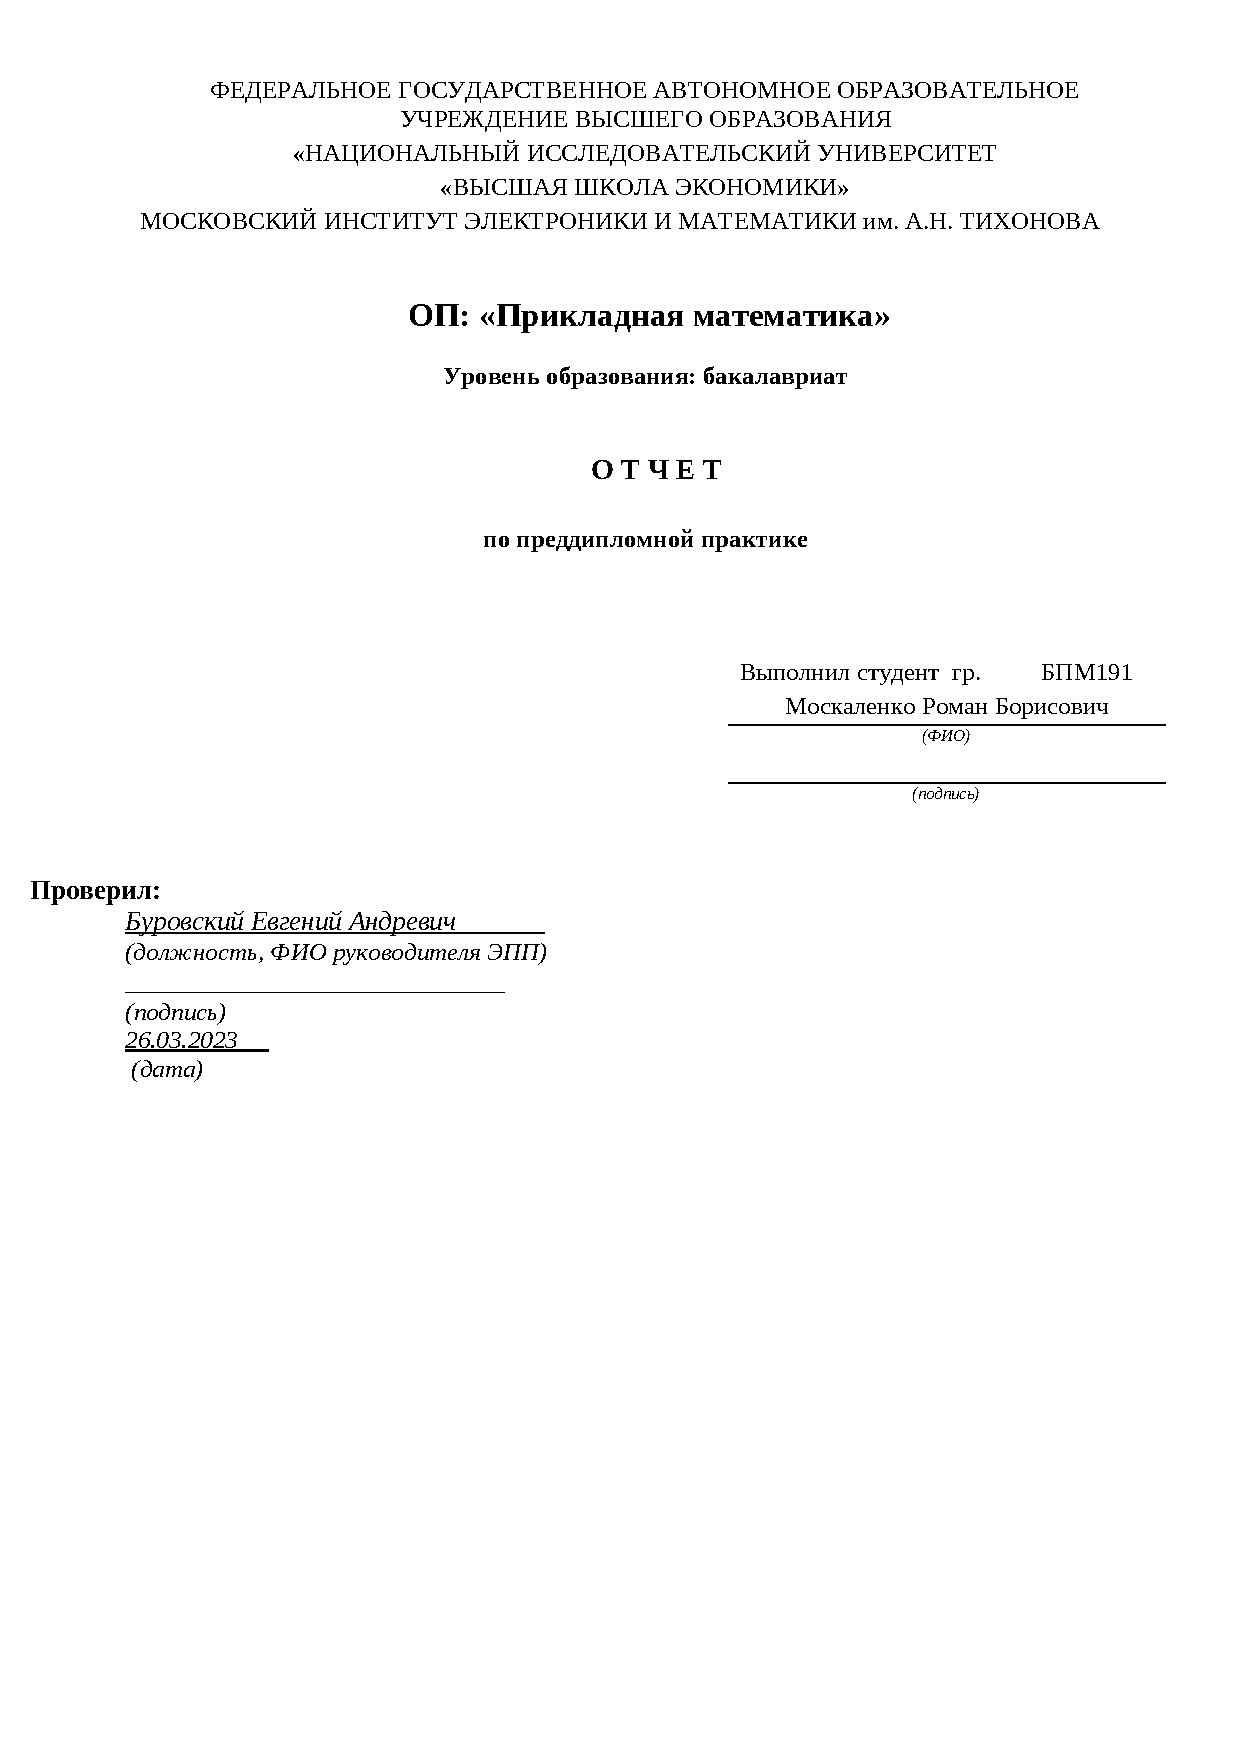
\includepdf{otchet_header.pdf}

\section{Введение}
%Модель Изинга используется для моделирования и изучения термодинамических свойств. Поведение структуры в модели Изинга сильно зависит от её геометрии. Так например на одно мерных моделях не происходит фазовый переход, но на двумерных моделях переход есть. Но что происходит в промежуточных размерностях? Например если взять какую-то последовательность узлов на двумерной решётке. Именно это и является главным вопросом в данном проекте. 
В данном проекте проводится исследование модели Изинга на фиксированной двумерной конформации. 

Возьмём конформацию(связанную не само пересекающуюся последовательность узлов) на двумерной решётке. Такие конформации можно рассматривать как термодинамическую систему, основанную на модели Изинга, для которых существуют две фазы: плотная(глобулярная) и развёрнутая. Эти фазы соответствуют низким и высоким температурам системы.

\begin{figure}[h]
	\centering
	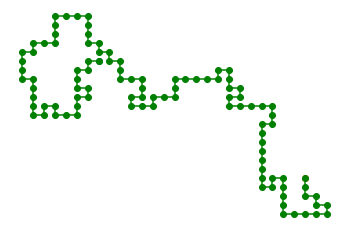
\includegraphics[width=0.45\textwidth]{../images/loose_conf.png}
	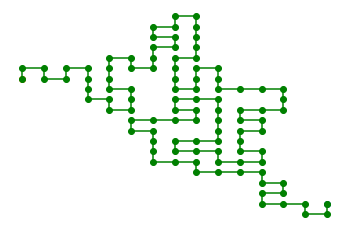
\includegraphics[width=0.45\textwidth]{../images/dense_conf.png} 
	\caption{Пример неплотной и плотной конформации}
\end{figure}

Если посмотреть на изображения конформаций каждого вида, хорошо видно, что плотные конформации по структуре близки с двумерным решёткам, где у каждого узла имеется множество соседей, и развёрнутые конформации наоборот близки к одномерным структурам, где узлы у которых больше 2 соседей встречаются редко. Соответственно можно предположить, что плотные конформации будут иметь свойства схожие с двумерными решётками, а развёрнутые с одномерными.


\subsection{Модель изинга}
Будем рассматривать конформацю как модель Изинга. В каждом узле конформации размещён спин $s_i$ принимающий значения $+1, -1$. Внешнее поле отсутствует. Гамильтониан системы $H = -J\sum_{i, j} s_i s_j$ где $i, j$ индексы соседних узлов, $J$ - коэффициент взаимодействия.

\subsection{Метод Монте-Карло}
Для моделирования системы используется метод Монте-Карло. Мною были реализованы версии с односпиновым и кластернным апдейтом, однако для измерений я использовал кластерную версию. Благодаря отказоустойчивости она работает значительно быстрее, и быстрее сходится, особенно при низких температурах.

На каждой итерации мы выбираем случайный спин и начиная с него начинаем строить кластер из одинаково направленных спинов, добавляя новые спины в кластер с определённой вероятностью. затем мы меняем значения спинов в кластере на противоположные.

% \section{Алгоритмы}

Реализованы два алгоритма обновления спинов. Односпиновый и кластерный апдейт. Оба алгоритма работают на произвольном графе, используя таблицу соседей. Алгоритмы реализованы как отдельные библиотеки для Python, и написаны с использованием технологии Cython для ускорения работы. Кластерный апдейт является более эффективным по времени работы и количеству шагов, которые необходимо выполнить для хорошей сходимости модели.

\subsection{Проверка алгоритмов}

Чтобы убедиться что алгоритмы работают правильно мы проверили, что оба алгоритма дают одинаковые результаты на одних и тех же конформациях, так же сравнил их с точными решениями для одномерной модели Изинга.

Результаты замеров кластерным и односпиновым апдейтом совпадают в пределах погрешности.

\begin{figure}[H]
	\centering
	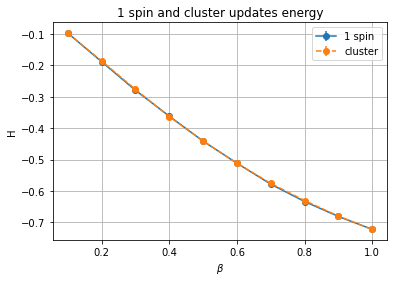
\includegraphics[width = 0.45\textwidth]{../images/1spin_&_cluster_ene.png} 
	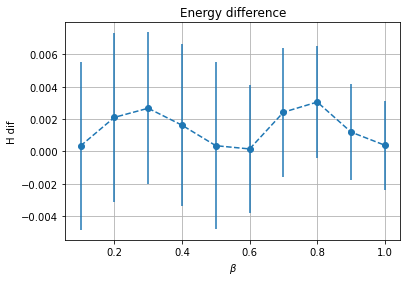
\includegraphics[width = 0.45\textwidth]{../images/1spin_&_cluster_ene_dif.png} 
	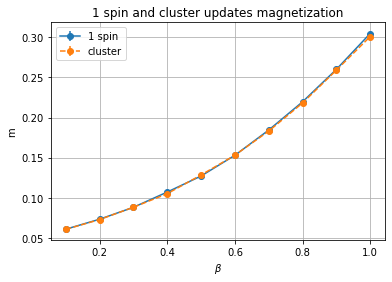
\includegraphics[width = 0.45\textwidth]{../images/1spin_&_cluster_mag.png} 
	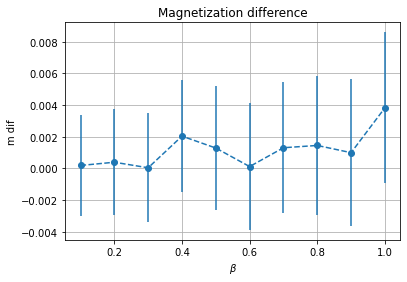
\includegraphics[width = 0.45\textwidth]{../images/1spin_&_cluster_mag_dif.png} 
	%% add magnetization
	\caption{кластерный и односпиновый апдейт}
\end{figure}

Для сравнения с точными значениями для одномерной модели Изинга, мы используем замкнутый квадратный контур. Данная конформация по свойствам полностью совпадает с одномерной моделью Изинга с открытыми граничными условиями.

\begin{figure}[H]
	\centering
	\begin{subfigure}[t]{0.45\textwidth}
		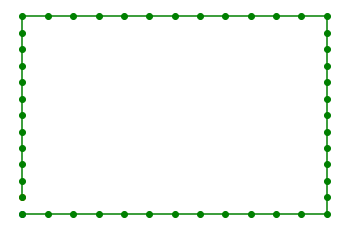
\includegraphics[width = \textwidth]{../images/1D_conf.png} 
		\caption{Конформация эмитирующая одномерную модель}
	\end{subfigure}
	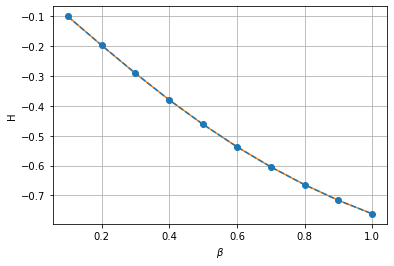
\includegraphics[width = 0.45\textwidth]{../images/1D_ene.png}
	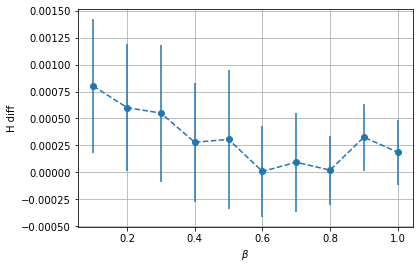
\includegraphics[width = 0.45\textwidth]{../images/1D_ene_diff.png} 
	%% add magnetization
	\caption{Сравнение с точным решением одномерной модели}
\end{figure}

Так же был написан код, точно вычисляющий энергию системы путём полного перебора всех её состояний. Сравнение на маленьких конформациях (длина 10) даёт одинаковые результаты.

%TODO втавить результаты поного перебора

Примеры с использованием кластерного апдейта добавлены в библиотеку \texttt{mc\_lib}.
\subsection{Текущие задачи}
\paragraph{Магнитная восприимчивость клубков}
Для определения точки магнитного перехода в конформациях мы используем магнитную восприимчивость. В точке магнитного перехода, магнитная восприимчивость должна иметь пи. И наоборот, если магнитный фазовый переход отсутствует, магнитная восприимчивость не должна иметь пиков. Так как мы предполагаем, что конформации вида клубок не имеют фазового магнитного перехода, мы хотим проверить что у них так же отсутствуют пики магнитной восприимчивости. Так же мы хотим сравнить магнитную восприимчивость конформаций клубок и одномерной модели изинга. 

\paragraph{Кластеризованные конформации}
Так же ранее было обнаружено что наличие в структуре конформации кластеров, отделённых от остальной части конформации одномерными цепочками, оказывает большое влияние на её магнитные свойства. Например даже плотные конформации могут иметь низкую намагниченность, если большая их часть разбита на два кластера равных размеров.

Мы рассмотрели влияние такой кластеризации на магнитные свойства конформаций, на сгенерированных наборах, которые мы рассматривали для определения точки перехода. Однако для более подробного изучения влияния кластеризации на магнитные свойства, будет эффективнее рассматривать специально сгенерированные конформации, с желаемой нам структурой.

\section{Магнитная восприимчивость клубков}
Магнитная восприимчивость это отношения изменения намагниченности к изменению внешнего магнитного поля. В пиках магнитной восприимчивости должна находится точка перехода.

Магнитная восприимчивость для данной модели вычисляется по следующей формуле.
\[
	\chi = \frac{\partial\langle |M|\rangle}{\partial h} = \beta \left(\langle M^2\rangle - \langle |M| \rangle^2 \right)
\]
Для одномерной цепочки Изинга с открытыми граничными условиями существует точное решение из которого можно вывести формулу Магнитной восприимчивости

\[
    \chi = \frac{\beta}{2} (2Ne^{2\beta J} - e^{4\beta J} + 1) + \frac{\beta}{2} \tanh^{N-1}(\beta J)(e^{4\beta J} - 2 e^{2\beta J} + 1)
\]
Где $N$ это количество спинов в цепочке. 

Мы рассмотрели конформации длинны 250, 500, 1000, 2000, по 1000 конформаций каждой длины

Действительно,у большинства конформаций полученных при $U=0.1$ отсутствуют пики, и график магнитной восприимчивости имеет такой же вид как и у одномерной модели изинига. Пример графиков представлен на рис. \ref{fig:MS_1D_comparison}. На этом же графике представлен пример масштабирования магнитной восприимчивости конформации, для сравнения с одномерной цепочкой.

\begin{figure}[ht]
	\centering
	%% Creator: Matplotlib, PGF backend
%%
%% To include the figure in your LaTeX document, write
%%   \input{<filename>.pgf}
%%
%% Make sure the required packages are loaded in your preamble
%%   \usepackage{pgf}
%%
%% Also ensure that all the required font packages are loaded; for instance,
%% the lmodern package is sometimes necessary when using math font.
%%   \usepackage{lmodern}
%%
%% Figures using additional raster images can only be included by \input if
%% they are in the same directory as the main LaTeX file. For loading figures
%% from other directories you can use the `import` package
%%   \usepackage{import}
%%
%% and then include the figures with
%%   \import{<path to file>}{<filename>.pgf}
%%
%% Matplotlib used the following preamble
%%   
%%   \usepackage{fontspec}
%%   \setmainfont{DejaVuSerif.ttf}[Path=\detokenize{/home/roman/anaconda3/envs/ising/lib/python3.8/site-packages/matplotlib/mpl-data/fonts/ttf/}]
%%   \setsansfont{DejaVuSans.ttf}[Path=\detokenize{/home/roman/anaconda3/envs/ising/lib/python3.8/site-packages/matplotlib/mpl-data/fonts/ttf/}]
%%   \setmonofont{DejaVuSansMono.ttf}[Path=\detokenize{/home/roman/anaconda3/envs/ising/lib/python3.8/site-packages/matplotlib/mpl-data/fonts/ttf/}]
%%   \makeatletter\@ifpackageloaded{underscore}{}{\usepackage[strings]{underscore}}\makeatother
%%
\begingroup%
\makeatletter%
\begin{pgfpicture}%
\pgfpathrectangle{\pgfpointorigin}{\pgfqpoint{5.217998in}{2.115535in}}%
\pgfusepath{use as bounding box, clip}%
\begin{pgfscope}%
\pgfsetbuttcap%
\pgfsetmiterjoin%
\definecolor{currentfill}{rgb}{1.000000,1.000000,1.000000}%
\pgfsetfillcolor{currentfill}%
\pgfsetlinewidth{0.000000pt}%
\definecolor{currentstroke}{rgb}{1.000000,1.000000,1.000000}%
\pgfsetstrokecolor{currentstroke}%
\pgfsetdash{}{0pt}%
\pgfpathmoveto{\pgfqpoint{0.000000in}{0.000000in}}%
\pgfpathlineto{\pgfqpoint{5.217998in}{0.000000in}}%
\pgfpathlineto{\pgfqpoint{5.217998in}{2.115535in}}%
\pgfpathlineto{\pgfqpoint{0.000000in}{2.115535in}}%
\pgfpathlineto{\pgfqpoint{0.000000in}{0.000000in}}%
\pgfpathclose%
\pgfusepath{fill}%
\end{pgfscope}%
\begin{pgfscope}%
\pgfsetbuttcap%
\pgfsetmiterjoin%
\definecolor{currentfill}{rgb}{1.000000,1.000000,1.000000}%
\pgfsetfillcolor{currentfill}%
\pgfsetlinewidth{0.000000pt}%
\definecolor{currentstroke}{rgb}{0.000000,0.000000,0.000000}%
\pgfsetstrokecolor{currentstroke}%
\pgfsetstrokeopacity{0.000000}%
\pgfsetdash{}{0pt}%
\pgfpathmoveto{\pgfqpoint{0.678396in}{0.467838in}}%
\pgfpathlineto{\pgfqpoint{2.696397in}{0.467838in}}%
\pgfpathlineto{\pgfqpoint{2.696397in}{1.830900in}}%
\pgfpathlineto{\pgfqpoint{0.678396in}{1.830900in}}%
\pgfpathlineto{\pgfqpoint{0.678396in}{0.467838in}}%
\pgfpathclose%
\pgfusepath{fill}%
\end{pgfscope}%
\begin{pgfscope}%
\pgfsetbuttcap%
\pgfsetroundjoin%
\definecolor{currentfill}{rgb}{0.000000,0.000000,0.000000}%
\pgfsetfillcolor{currentfill}%
\pgfsetlinewidth{0.803000pt}%
\definecolor{currentstroke}{rgb}{0.000000,0.000000,0.000000}%
\pgfsetstrokecolor{currentstroke}%
\pgfsetdash{}{0pt}%
\pgfsys@defobject{currentmarker}{\pgfqpoint{0.000000in}{-0.048611in}}{\pgfqpoint{0.000000in}{0.000000in}}{%
\pgfpathmoveto{\pgfqpoint{0.000000in}{0.000000in}}%
\pgfpathlineto{\pgfqpoint{0.000000in}{-0.048611in}}%
\pgfusepath{stroke,fill}%
}%
\begin{pgfscope}%
\pgfsys@transformshift{0.973962in}{0.467838in}%
\pgfsys@useobject{currentmarker}{}%
\end{pgfscope}%
\end{pgfscope}%
\begin{pgfscope}%
\definecolor{textcolor}{rgb}{0.000000,0.000000,0.000000}%
\pgfsetstrokecolor{textcolor}%
\pgfsetfillcolor{textcolor}%
\pgftext[x=0.973962in,y=0.370616in,,top]{\color{textcolor}\sffamily\fontsize{8.000000}{9.600000}\selectfont 0.2}%
\end{pgfscope}%
\begin{pgfscope}%
\pgfsetbuttcap%
\pgfsetroundjoin%
\definecolor{currentfill}{rgb}{0.000000,0.000000,0.000000}%
\pgfsetfillcolor{currentfill}%
\pgfsetlinewidth{0.803000pt}%
\definecolor{currentstroke}{rgb}{0.000000,0.000000,0.000000}%
\pgfsetstrokecolor{currentstroke}%
\pgfsetdash{}{0pt}%
\pgfsys@defobject{currentmarker}{\pgfqpoint{0.000000in}{-0.048611in}}{\pgfqpoint{0.000000in}{0.000000in}}{%
\pgfpathmoveto{\pgfqpoint{0.000000in}{0.000000in}}%
\pgfpathlineto{\pgfqpoint{0.000000in}{-0.048611in}}%
\pgfusepath{stroke,fill}%
}%
\begin{pgfscope}%
\pgfsys@transformshift{1.381639in}{0.467838in}%
\pgfsys@useobject{currentmarker}{}%
\end{pgfscope}%
\end{pgfscope}%
\begin{pgfscope}%
\definecolor{textcolor}{rgb}{0.000000,0.000000,0.000000}%
\pgfsetstrokecolor{textcolor}%
\pgfsetfillcolor{textcolor}%
\pgftext[x=1.381639in,y=0.370616in,,top]{\color{textcolor}\sffamily\fontsize{8.000000}{9.600000}\selectfont 0.4}%
\end{pgfscope}%
\begin{pgfscope}%
\pgfsetbuttcap%
\pgfsetroundjoin%
\definecolor{currentfill}{rgb}{0.000000,0.000000,0.000000}%
\pgfsetfillcolor{currentfill}%
\pgfsetlinewidth{0.803000pt}%
\definecolor{currentstroke}{rgb}{0.000000,0.000000,0.000000}%
\pgfsetstrokecolor{currentstroke}%
\pgfsetdash{}{0pt}%
\pgfsys@defobject{currentmarker}{\pgfqpoint{0.000000in}{-0.048611in}}{\pgfqpoint{0.000000in}{0.000000in}}{%
\pgfpathmoveto{\pgfqpoint{0.000000in}{0.000000in}}%
\pgfpathlineto{\pgfqpoint{0.000000in}{-0.048611in}}%
\pgfusepath{stroke,fill}%
}%
\begin{pgfscope}%
\pgfsys@transformshift{1.789316in}{0.467838in}%
\pgfsys@useobject{currentmarker}{}%
\end{pgfscope}%
\end{pgfscope}%
\begin{pgfscope}%
\definecolor{textcolor}{rgb}{0.000000,0.000000,0.000000}%
\pgfsetstrokecolor{textcolor}%
\pgfsetfillcolor{textcolor}%
\pgftext[x=1.789316in,y=0.370616in,,top]{\color{textcolor}\sffamily\fontsize{8.000000}{9.600000}\selectfont 0.6}%
\end{pgfscope}%
\begin{pgfscope}%
\pgfsetbuttcap%
\pgfsetroundjoin%
\definecolor{currentfill}{rgb}{0.000000,0.000000,0.000000}%
\pgfsetfillcolor{currentfill}%
\pgfsetlinewidth{0.803000pt}%
\definecolor{currentstroke}{rgb}{0.000000,0.000000,0.000000}%
\pgfsetstrokecolor{currentstroke}%
\pgfsetdash{}{0pt}%
\pgfsys@defobject{currentmarker}{\pgfqpoint{0.000000in}{-0.048611in}}{\pgfqpoint{0.000000in}{0.000000in}}{%
\pgfpathmoveto{\pgfqpoint{0.000000in}{0.000000in}}%
\pgfpathlineto{\pgfqpoint{0.000000in}{-0.048611in}}%
\pgfusepath{stroke,fill}%
}%
\begin{pgfscope}%
\pgfsys@transformshift{2.196993in}{0.467838in}%
\pgfsys@useobject{currentmarker}{}%
\end{pgfscope}%
\end{pgfscope}%
\begin{pgfscope}%
\definecolor{textcolor}{rgb}{0.000000,0.000000,0.000000}%
\pgfsetstrokecolor{textcolor}%
\pgfsetfillcolor{textcolor}%
\pgftext[x=2.196993in,y=0.370616in,,top]{\color{textcolor}\sffamily\fontsize{8.000000}{9.600000}\selectfont 0.8}%
\end{pgfscope}%
\begin{pgfscope}%
\pgfsetbuttcap%
\pgfsetroundjoin%
\definecolor{currentfill}{rgb}{0.000000,0.000000,0.000000}%
\pgfsetfillcolor{currentfill}%
\pgfsetlinewidth{0.803000pt}%
\definecolor{currentstroke}{rgb}{0.000000,0.000000,0.000000}%
\pgfsetstrokecolor{currentstroke}%
\pgfsetdash{}{0pt}%
\pgfsys@defobject{currentmarker}{\pgfqpoint{0.000000in}{-0.048611in}}{\pgfqpoint{0.000000in}{0.000000in}}{%
\pgfpathmoveto{\pgfqpoint{0.000000in}{0.000000in}}%
\pgfpathlineto{\pgfqpoint{0.000000in}{-0.048611in}}%
\pgfusepath{stroke,fill}%
}%
\begin{pgfscope}%
\pgfsys@transformshift{2.604669in}{0.467838in}%
\pgfsys@useobject{currentmarker}{}%
\end{pgfscope}%
\end{pgfscope}%
\begin{pgfscope}%
\definecolor{textcolor}{rgb}{0.000000,0.000000,0.000000}%
\pgfsetstrokecolor{textcolor}%
\pgfsetfillcolor{textcolor}%
\pgftext[x=2.604669in,y=0.370616in,,top]{\color{textcolor}\sffamily\fontsize{8.000000}{9.600000}\selectfont 1.0}%
\end{pgfscope}%
\begin{pgfscope}%
\definecolor{textcolor}{rgb}{0.000000,0.000000,0.000000}%
\pgfsetstrokecolor{textcolor}%
\pgfsetfillcolor{textcolor}%
\pgftext[x=1.687396in,y=0.207530in,,top]{\color{textcolor}\sffamily\fontsize{8.000000}{9.600000}\selectfont \(\displaystyle \beta\)}%
\end{pgfscope}%
\begin{pgfscope}%
\pgfsetbuttcap%
\pgfsetroundjoin%
\definecolor{currentfill}{rgb}{0.000000,0.000000,0.000000}%
\pgfsetfillcolor{currentfill}%
\pgfsetlinewidth{0.803000pt}%
\definecolor{currentstroke}{rgb}{0.000000,0.000000,0.000000}%
\pgfsetstrokecolor{currentstroke}%
\pgfsetdash{}{0pt}%
\pgfsys@defobject{currentmarker}{\pgfqpoint{-0.048611in}{0.000000in}}{\pgfqpoint{-0.000000in}{0.000000in}}{%
\pgfpathmoveto{\pgfqpoint{-0.000000in}{0.000000in}}%
\pgfpathlineto{\pgfqpoint{-0.048611in}{0.000000in}}%
\pgfusepath{stroke,fill}%
}%
\begin{pgfscope}%
\pgfsys@transformshift{0.678396in}{0.521526in}%
\pgfsys@useobject{currentmarker}{}%
\end{pgfscope}%
\end{pgfscope}%
\begin{pgfscope}%
\definecolor{textcolor}{rgb}{0.000000,0.000000,0.000000}%
\pgfsetstrokecolor{textcolor}%
\pgfsetfillcolor{textcolor}%
\pgftext[x=0.263086in, y=0.479317in, left, base]{\color{textcolor}\sffamily\fontsize{8.000000}{9.600000}\selectfont 0.000}%
\end{pgfscope}%
\begin{pgfscope}%
\pgfsetbuttcap%
\pgfsetroundjoin%
\definecolor{currentfill}{rgb}{0.000000,0.000000,0.000000}%
\pgfsetfillcolor{currentfill}%
\pgfsetlinewidth{0.803000pt}%
\definecolor{currentstroke}{rgb}{0.000000,0.000000,0.000000}%
\pgfsetstrokecolor{currentstroke}%
\pgfsetdash{}{0pt}%
\pgfsys@defobject{currentmarker}{\pgfqpoint{-0.048611in}{0.000000in}}{\pgfqpoint{-0.000000in}{0.000000in}}{%
\pgfpathmoveto{\pgfqpoint{-0.000000in}{0.000000in}}%
\pgfpathlineto{\pgfqpoint{-0.048611in}{0.000000in}}%
\pgfusepath{stroke,fill}%
}%
\begin{pgfscope}%
\pgfsys@transformshift{0.678396in}{0.860732in}%
\pgfsys@useobject{currentmarker}{}%
\end{pgfscope}%
\end{pgfscope}%
\begin{pgfscope}%
\definecolor{textcolor}{rgb}{0.000000,0.000000,0.000000}%
\pgfsetstrokecolor{textcolor}%
\pgfsetfillcolor{textcolor}%
\pgftext[x=0.263086in, y=0.818522in, left, base]{\color{textcolor}\sffamily\fontsize{8.000000}{9.600000}\selectfont 0.002}%
\end{pgfscope}%
\begin{pgfscope}%
\pgfsetbuttcap%
\pgfsetroundjoin%
\definecolor{currentfill}{rgb}{0.000000,0.000000,0.000000}%
\pgfsetfillcolor{currentfill}%
\pgfsetlinewidth{0.803000pt}%
\definecolor{currentstroke}{rgb}{0.000000,0.000000,0.000000}%
\pgfsetstrokecolor{currentstroke}%
\pgfsetdash{}{0pt}%
\pgfsys@defobject{currentmarker}{\pgfqpoint{-0.048611in}{0.000000in}}{\pgfqpoint{-0.000000in}{0.000000in}}{%
\pgfpathmoveto{\pgfqpoint{-0.000000in}{0.000000in}}%
\pgfpathlineto{\pgfqpoint{-0.048611in}{0.000000in}}%
\pgfusepath{stroke,fill}%
}%
\begin{pgfscope}%
\pgfsys@transformshift{0.678396in}{1.199937in}%
\pgfsys@useobject{currentmarker}{}%
\end{pgfscope}%
\end{pgfscope}%
\begin{pgfscope}%
\definecolor{textcolor}{rgb}{0.000000,0.000000,0.000000}%
\pgfsetstrokecolor{textcolor}%
\pgfsetfillcolor{textcolor}%
\pgftext[x=0.263086in, y=1.157728in, left, base]{\color{textcolor}\sffamily\fontsize{8.000000}{9.600000}\selectfont 0.004}%
\end{pgfscope}%
\begin{pgfscope}%
\pgfsetbuttcap%
\pgfsetroundjoin%
\definecolor{currentfill}{rgb}{0.000000,0.000000,0.000000}%
\pgfsetfillcolor{currentfill}%
\pgfsetlinewidth{0.803000pt}%
\definecolor{currentstroke}{rgb}{0.000000,0.000000,0.000000}%
\pgfsetstrokecolor{currentstroke}%
\pgfsetdash{}{0pt}%
\pgfsys@defobject{currentmarker}{\pgfqpoint{-0.048611in}{0.000000in}}{\pgfqpoint{-0.000000in}{0.000000in}}{%
\pgfpathmoveto{\pgfqpoint{-0.000000in}{0.000000in}}%
\pgfpathlineto{\pgfqpoint{-0.048611in}{0.000000in}}%
\pgfusepath{stroke,fill}%
}%
\begin{pgfscope}%
\pgfsys@transformshift{0.678396in}{1.539143in}%
\pgfsys@useobject{currentmarker}{}%
\end{pgfscope}%
\end{pgfscope}%
\begin{pgfscope}%
\definecolor{textcolor}{rgb}{0.000000,0.000000,0.000000}%
\pgfsetstrokecolor{textcolor}%
\pgfsetfillcolor{textcolor}%
\pgftext[x=0.263086in, y=1.496933in, left, base]{\color{textcolor}\sffamily\fontsize{8.000000}{9.600000}\selectfont 0.006}%
\end{pgfscope}%
\begin{pgfscope}%
\definecolor{textcolor}{rgb}{0.000000,0.000000,0.000000}%
\pgfsetstrokecolor{textcolor}%
\pgfsetfillcolor{textcolor}%
\pgftext[x=0.207530in,y=1.149369in,,bottom,rotate=90.000000]{\color{textcolor}\sffamily\fontsize{8.000000}{9.600000}\selectfont \(\displaystyle X\)}%
\end{pgfscope}%
\begin{pgfscope}%
\pgfpathrectangle{\pgfqpoint{0.678396in}{0.467838in}}{\pgfqpoint{2.018001in}{1.363061in}}%
\pgfusepath{clip}%
\pgfsetrectcap%
\pgfsetroundjoin%
\pgfsetlinewidth{1.505625pt}%
\definecolor{currentstroke}{rgb}{0.000000,0.000000,0.000000}%
\pgfsetstrokecolor{currentstroke}%
\pgfsetdash{}{0pt}%
\pgfpathmoveto{\pgfqpoint{0.770123in}{0.542217in}}%
\pgfpathlineto{\pgfqpoint{0.973962in}{0.572058in}}%
\pgfpathlineto{\pgfqpoint{1.177800in}{0.614085in}}%
\pgfpathlineto{\pgfqpoint{1.381639in}{0.672225in}}%
\pgfpathlineto{\pgfqpoint{1.585477in}{0.751539in}}%
\pgfpathlineto{\pgfqpoint{1.789316in}{0.858540in}}%
\pgfpathlineto{\pgfqpoint{1.993154in}{1.001571in}}%
\pgfpathlineto{\pgfqpoint{2.196993in}{1.191300in}}%
\pgfpathlineto{\pgfqpoint{2.400831in}{1.441325in}}%
\pgfpathlineto{\pgfqpoint{2.604669in}{1.768942in}}%
\pgfusepath{stroke}%
\end{pgfscope}%
\begin{pgfscope}%
\pgfpathrectangle{\pgfqpoint{0.678396in}{0.467838in}}{\pgfqpoint{2.018001in}{1.363061in}}%
\pgfusepath{clip}%
\pgfsetrectcap%
\pgfsetroundjoin%
\pgfsetlinewidth{1.505625pt}%
\definecolor{currentstroke}{rgb}{0.121569,0.466667,0.705882}%
\pgfsetstrokecolor{currentstroke}%
\pgfsetdash{}{0pt}%
\pgfpathmoveto{\pgfqpoint{0.770123in}{0.529796in}}%
\pgfpathlineto{\pgfqpoint{0.973962in}{0.542041in}}%
\pgfpathlineto{\pgfqpoint{1.177800in}{0.563116in}}%
\pgfpathlineto{\pgfqpoint{1.381639in}{0.596044in}}%
\pgfpathlineto{\pgfqpoint{1.585477in}{0.651218in}}%
\pgfpathlineto{\pgfqpoint{1.789316in}{0.735119in}}%
\pgfpathlineto{\pgfqpoint{1.993154in}{0.860588in}}%
\pgfpathlineto{\pgfqpoint{2.196993in}{1.015296in}}%
\pgfpathlineto{\pgfqpoint{2.400831in}{1.213409in}}%
\pgfpathlineto{\pgfqpoint{2.604669in}{1.487094in}}%
\pgfusepath{stroke}%
\end{pgfscope}%
\begin{pgfscope}%
\pgfsetrectcap%
\pgfsetmiterjoin%
\pgfsetlinewidth{0.803000pt}%
\definecolor{currentstroke}{rgb}{0.000000,0.000000,0.000000}%
\pgfsetstrokecolor{currentstroke}%
\pgfsetdash{}{0pt}%
\pgfpathmoveto{\pgfqpoint{0.678396in}{0.467838in}}%
\pgfpathlineto{\pgfqpoint{0.678396in}{1.830900in}}%
\pgfusepath{stroke}%
\end{pgfscope}%
\begin{pgfscope}%
\pgfsetrectcap%
\pgfsetmiterjoin%
\pgfsetlinewidth{0.803000pt}%
\definecolor{currentstroke}{rgb}{0.000000,0.000000,0.000000}%
\pgfsetstrokecolor{currentstroke}%
\pgfsetdash{}{0pt}%
\pgfpathmoveto{\pgfqpoint{2.696397in}{0.467838in}}%
\pgfpathlineto{\pgfqpoint{2.696397in}{1.830900in}}%
\pgfusepath{stroke}%
\end{pgfscope}%
\begin{pgfscope}%
\pgfsetrectcap%
\pgfsetmiterjoin%
\pgfsetlinewidth{0.803000pt}%
\definecolor{currentstroke}{rgb}{0.000000,0.000000,0.000000}%
\pgfsetstrokecolor{currentstroke}%
\pgfsetdash{}{0pt}%
\pgfpathmoveto{\pgfqpoint{0.678396in}{0.467838in}}%
\pgfpathlineto{\pgfqpoint{2.696397in}{0.467838in}}%
\pgfusepath{stroke}%
\end{pgfscope}%
\begin{pgfscope}%
\pgfsetrectcap%
\pgfsetmiterjoin%
\pgfsetlinewidth{0.803000pt}%
\definecolor{currentstroke}{rgb}{0.000000,0.000000,0.000000}%
\pgfsetstrokecolor{currentstroke}%
\pgfsetdash{}{0pt}%
\pgfpathmoveto{\pgfqpoint{0.678396in}{1.830900in}}%
\pgfpathlineto{\pgfqpoint{2.696397in}{1.830900in}}%
\pgfusepath{stroke}%
\end{pgfscope}%
\begin{pgfscope}%
\definecolor{textcolor}{rgb}{0.000000,0.000000,0.000000}%
\pgfsetstrokecolor{textcolor}%
\pgfsetfillcolor{textcolor}%
\pgftext[x=1.687396in,y=1.914233in,,base]{\color{textcolor}\sffamily\fontsize{9.600000}{11.520000}\selectfont original values}%
\end{pgfscope}%
\begin{pgfscope}%
\pgfsetbuttcap%
\pgfsetmiterjoin%
\definecolor{currentfill}{rgb}{1.000000,1.000000,1.000000}%
\pgfsetfillcolor{currentfill}%
\pgfsetfillopacity{0.800000}%
\pgfsetlinewidth{1.003750pt}%
\definecolor{currentstroke}{rgb}{0.800000,0.800000,0.800000}%
\pgfsetstrokecolor{currentstroke}%
\pgfsetstrokeopacity{0.800000}%
\pgfsetdash{}{0pt}%
\pgfpathmoveto{\pgfqpoint{0.756174in}{1.415839in}}%
\pgfpathlineto{\pgfqpoint{1.851204in}{1.415839in}}%
\pgfpathquadraticcurveto{\pgfqpoint{1.873427in}{1.415839in}}{\pgfqpoint{1.873427in}{1.438061in}}%
\pgfpathlineto{\pgfqpoint{1.873427in}{1.753122in}}%
\pgfpathquadraticcurveto{\pgfqpoint{1.873427in}{1.775344in}}{\pgfqpoint{1.851204in}{1.775344in}}%
\pgfpathlineto{\pgfqpoint{0.756174in}{1.775344in}}%
\pgfpathquadraticcurveto{\pgfqpoint{0.733952in}{1.775344in}}{\pgfqpoint{0.733952in}{1.753122in}}%
\pgfpathlineto{\pgfqpoint{0.733952in}{1.438061in}}%
\pgfpathquadraticcurveto{\pgfqpoint{0.733952in}{1.415839in}}{\pgfqpoint{0.756174in}{1.415839in}}%
\pgfpathlineto{\pgfqpoint{0.756174in}{1.415839in}}%
\pgfpathclose%
\pgfusepath{stroke,fill}%
\end{pgfscope}%
\begin{pgfscope}%
\pgfsetrectcap%
\pgfsetroundjoin%
\pgfsetlinewidth{1.505625pt}%
\definecolor{currentstroke}{rgb}{0.000000,0.000000,0.000000}%
\pgfsetstrokecolor{currentstroke}%
\pgfsetdash{}{0pt}%
\pgfpathmoveto{\pgfqpoint{0.778396in}{1.685370in}}%
\pgfpathlineto{\pgfqpoint{0.889507in}{1.685370in}}%
\pgfpathlineto{\pgfqpoint{1.000618in}{1.685370in}}%
\pgfusepath{stroke}%
\end{pgfscope}%
\begin{pgfscope}%
\definecolor{textcolor}{rgb}{0.000000,0.000000,0.000000}%
\pgfsetstrokecolor{textcolor}%
\pgfsetfillcolor{textcolor}%
\pgftext[x=1.089507in,y=1.646481in,left,base]{\color{textcolor}\sffamily\fontsize{8.000000}{9.600000}\selectfont exact 1D}%
\end{pgfscope}%
\begin{pgfscope}%
\pgfsetrectcap%
\pgfsetroundjoin%
\pgfsetlinewidth{1.505625pt}%
\definecolor{currentstroke}{rgb}{0.121569,0.466667,0.705882}%
\pgfsetstrokecolor{currentstroke}%
\pgfsetdash{}{0pt}%
\pgfpathmoveto{\pgfqpoint{0.778396in}{1.522284in}}%
\pgfpathlineto{\pgfqpoint{0.889507in}{1.522284in}}%
\pgfpathlineto{\pgfqpoint{1.000618in}{1.522284in}}%
\pgfusepath{stroke}%
\end{pgfscope}%
\begin{pgfscope}%
\definecolor{textcolor}{rgb}{0.000000,0.000000,0.000000}%
\pgfsetstrokecolor{textcolor}%
\pgfsetfillcolor{textcolor}%
\pgftext[x=1.089507in,y=1.483395in,left,base]{\color{textcolor}\sffamily\fontsize{8.000000}{9.600000}\selectfont conformation}%
\end{pgfscope}%
\begin{pgfscope}%
\pgfsetbuttcap%
\pgfsetmiterjoin%
\definecolor{currentfill}{rgb}{1.000000,1.000000,1.000000}%
\pgfsetfillcolor{currentfill}%
\pgfsetlinewidth{0.000000pt}%
\definecolor{currentstroke}{rgb}{0.000000,0.000000,0.000000}%
\pgfsetstrokecolor{currentstroke}%
\pgfsetstrokeopacity{0.000000}%
\pgfsetdash{}{0pt}%
\pgfpathmoveto{\pgfqpoint{3.099997in}{0.467838in}}%
\pgfpathlineto{\pgfqpoint{5.117998in}{0.467838in}}%
\pgfpathlineto{\pgfqpoint{5.117998in}{1.830900in}}%
\pgfpathlineto{\pgfqpoint{3.099997in}{1.830900in}}%
\pgfpathlineto{\pgfqpoint{3.099997in}{0.467838in}}%
\pgfpathclose%
\pgfusepath{fill}%
\end{pgfscope}%
\begin{pgfscope}%
\pgfsetbuttcap%
\pgfsetroundjoin%
\definecolor{currentfill}{rgb}{0.000000,0.000000,0.000000}%
\pgfsetfillcolor{currentfill}%
\pgfsetlinewidth{0.803000pt}%
\definecolor{currentstroke}{rgb}{0.000000,0.000000,0.000000}%
\pgfsetstrokecolor{currentstroke}%
\pgfsetdash{}{0pt}%
\pgfsys@defobject{currentmarker}{\pgfqpoint{0.000000in}{-0.048611in}}{\pgfqpoint{0.000000in}{0.000000in}}{%
\pgfpathmoveto{\pgfqpoint{0.000000in}{0.000000in}}%
\pgfpathlineto{\pgfqpoint{0.000000in}{-0.048611in}}%
\pgfusepath{stroke,fill}%
}%
\begin{pgfscope}%
\pgfsys@transformshift{3.395563in}{0.467838in}%
\pgfsys@useobject{currentmarker}{}%
\end{pgfscope}%
\end{pgfscope}%
\begin{pgfscope}%
\definecolor{textcolor}{rgb}{0.000000,0.000000,0.000000}%
\pgfsetstrokecolor{textcolor}%
\pgfsetfillcolor{textcolor}%
\pgftext[x=3.395563in,y=0.370616in,,top]{\color{textcolor}\sffamily\fontsize{8.000000}{9.600000}\selectfont 0.2}%
\end{pgfscope}%
\begin{pgfscope}%
\pgfsetbuttcap%
\pgfsetroundjoin%
\definecolor{currentfill}{rgb}{0.000000,0.000000,0.000000}%
\pgfsetfillcolor{currentfill}%
\pgfsetlinewidth{0.803000pt}%
\definecolor{currentstroke}{rgb}{0.000000,0.000000,0.000000}%
\pgfsetstrokecolor{currentstroke}%
\pgfsetdash{}{0pt}%
\pgfsys@defobject{currentmarker}{\pgfqpoint{0.000000in}{-0.048611in}}{\pgfqpoint{0.000000in}{0.000000in}}{%
\pgfpathmoveto{\pgfqpoint{0.000000in}{0.000000in}}%
\pgfpathlineto{\pgfqpoint{0.000000in}{-0.048611in}}%
\pgfusepath{stroke,fill}%
}%
\begin{pgfscope}%
\pgfsys@transformshift{3.803240in}{0.467838in}%
\pgfsys@useobject{currentmarker}{}%
\end{pgfscope}%
\end{pgfscope}%
\begin{pgfscope}%
\definecolor{textcolor}{rgb}{0.000000,0.000000,0.000000}%
\pgfsetstrokecolor{textcolor}%
\pgfsetfillcolor{textcolor}%
\pgftext[x=3.803240in,y=0.370616in,,top]{\color{textcolor}\sffamily\fontsize{8.000000}{9.600000}\selectfont 0.4}%
\end{pgfscope}%
\begin{pgfscope}%
\pgfsetbuttcap%
\pgfsetroundjoin%
\definecolor{currentfill}{rgb}{0.000000,0.000000,0.000000}%
\pgfsetfillcolor{currentfill}%
\pgfsetlinewidth{0.803000pt}%
\definecolor{currentstroke}{rgb}{0.000000,0.000000,0.000000}%
\pgfsetstrokecolor{currentstroke}%
\pgfsetdash{}{0pt}%
\pgfsys@defobject{currentmarker}{\pgfqpoint{0.000000in}{-0.048611in}}{\pgfqpoint{0.000000in}{0.000000in}}{%
\pgfpathmoveto{\pgfqpoint{0.000000in}{0.000000in}}%
\pgfpathlineto{\pgfqpoint{0.000000in}{-0.048611in}}%
\pgfusepath{stroke,fill}%
}%
\begin{pgfscope}%
\pgfsys@transformshift{4.210916in}{0.467838in}%
\pgfsys@useobject{currentmarker}{}%
\end{pgfscope}%
\end{pgfscope}%
\begin{pgfscope}%
\definecolor{textcolor}{rgb}{0.000000,0.000000,0.000000}%
\pgfsetstrokecolor{textcolor}%
\pgfsetfillcolor{textcolor}%
\pgftext[x=4.210916in,y=0.370616in,,top]{\color{textcolor}\sffamily\fontsize{8.000000}{9.600000}\selectfont 0.6}%
\end{pgfscope}%
\begin{pgfscope}%
\pgfsetbuttcap%
\pgfsetroundjoin%
\definecolor{currentfill}{rgb}{0.000000,0.000000,0.000000}%
\pgfsetfillcolor{currentfill}%
\pgfsetlinewidth{0.803000pt}%
\definecolor{currentstroke}{rgb}{0.000000,0.000000,0.000000}%
\pgfsetstrokecolor{currentstroke}%
\pgfsetdash{}{0pt}%
\pgfsys@defobject{currentmarker}{\pgfqpoint{0.000000in}{-0.048611in}}{\pgfqpoint{0.000000in}{0.000000in}}{%
\pgfpathmoveto{\pgfqpoint{0.000000in}{0.000000in}}%
\pgfpathlineto{\pgfqpoint{0.000000in}{-0.048611in}}%
\pgfusepath{stroke,fill}%
}%
\begin{pgfscope}%
\pgfsys@transformshift{4.618593in}{0.467838in}%
\pgfsys@useobject{currentmarker}{}%
\end{pgfscope}%
\end{pgfscope}%
\begin{pgfscope}%
\definecolor{textcolor}{rgb}{0.000000,0.000000,0.000000}%
\pgfsetstrokecolor{textcolor}%
\pgfsetfillcolor{textcolor}%
\pgftext[x=4.618593in,y=0.370616in,,top]{\color{textcolor}\sffamily\fontsize{8.000000}{9.600000}\selectfont 0.8}%
\end{pgfscope}%
\begin{pgfscope}%
\pgfsetbuttcap%
\pgfsetroundjoin%
\definecolor{currentfill}{rgb}{0.000000,0.000000,0.000000}%
\pgfsetfillcolor{currentfill}%
\pgfsetlinewidth{0.803000pt}%
\definecolor{currentstroke}{rgb}{0.000000,0.000000,0.000000}%
\pgfsetstrokecolor{currentstroke}%
\pgfsetdash{}{0pt}%
\pgfsys@defobject{currentmarker}{\pgfqpoint{0.000000in}{-0.048611in}}{\pgfqpoint{0.000000in}{0.000000in}}{%
\pgfpathmoveto{\pgfqpoint{0.000000in}{0.000000in}}%
\pgfpathlineto{\pgfqpoint{0.000000in}{-0.048611in}}%
\pgfusepath{stroke,fill}%
}%
\begin{pgfscope}%
\pgfsys@transformshift{5.026270in}{0.467838in}%
\pgfsys@useobject{currentmarker}{}%
\end{pgfscope}%
\end{pgfscope}%
\begin{pgfscope}%
\definecolor{textcolor}{rgb}{0.000000,0.000000,0.000000}%
\pgfsetstrokecolor{textcolor}%
\pgfsetfillcolor{textcolor}%
\pgftext[x=5.026270in,y=0.370616in,,top]{\color{textcolor}\sffamily\fontsize{8.000000}{9.600000}\selectfont 1.0}%
\end{pgfscope}%
\begin{pgfscope}%
\definecolor{textcolor}{rgb}{0.000000,0.000000,0.000000}%
\pgfsetstrokecolor{textcolor}%
\pgfsetfillcolor{textcolor}%
\pgftext[x=4.108997in,y=0.207530in,,top]{\color{textcolor}\sffamily\fontsize{8.000000}{9.600000}\selectfont \(\displaystyle \beta\)}%
\end{pgfscope}%
\begin{pgfscope}%
\pgfsetbuttcap%
\pgfsetroundjoin%
\definecolor{currentfill}{rgb}{0.000000,0.000000,0.000000}%
\pgfsetfillcolor{currentfill}%
\pgfsetlinewidth{0.803000pt}%
\definecolor{currentstroke}{rgb}{0.000000,0.000000,0.000000}%
\pgfsetstrokecolor{currentstroke}%
\pgfsetdash{}{0pt}%
\pgfsys@defobject{currentmarker}{\pgfqpoint{-0.048611in}{0.000000in}}{\pgfqpoint{-0.000000in}{0.000000in}}{%
\pgfpathmoveto{\pgfqpoint{-0.000000in}{0.000000in}}%
\pgfpathlineto{\pgfqpoint{-0.048611in}{0.000000in}}%
\pgfusepath{stroke,fill}%
}%
\begin{pgfscope}%
\pgfsys@transformshift{3.099997in}{0.519091in}%
\pgfsys@useobject{currentmarker}{}%
\end{pgfscope}%
\end{pgfscope}%
\begin{pgfscope}%
\definecolor{textcolor}{rgb}{0.000000,0.000000,0.000000}%
\pgfsetstrokecolor{textcolor}%
\pgfsetfillcolor{textcolor}%
\pgftext[x=2.684687in, y=0.476882in, left, base]{\color{textcolor}\sffamily\fontsize{8.000000}{9.600000}\selectfont 0.000}%
\end{pgfscope}%
\begin{pgfscope}%
\pgfsetbuttcap%
\pgfsetroundjoin%
\definecolor{currentfill}{rgb}{0.000000,0.000000,0.000000}%
\pgfsetfillcolor{currentfill}%
\pgfsetlinewidth{0.803000pt}%
\definecolor{currentstroke}{rgb}{0.000000,0.000000,0.000000}%
\pgfsetstrokecolor{currentstroke}%
\pgfsetdash{}{0pt}%
\pgfsys@defobject{currentmarker}{\pgfqpoint{-0.048611in}{0.000000in}}{\pgfqpoint{-0.000000in}{0.000000in}}{%
\pgfpathmoveto{\pgfqpoint{-0.000000in}{0.000000in}}%
\pgfpathlineto{\pgfqpoint{-0.048611in}{0.000000in}}%
\pgfusepath{stroke,fill}%
}%
\begin{pgfscope}%
\pgfsys@transformshift{3.099997in}{0.848519in}%
\pgfsys@useobject{currentmarker}{}%
\end{pgfscope}%
\end{pgfscope}%
\begin{pgfscope}%
\definecolor{textcolor}{rgb}{0.000000,0.000000,0.000000}%
\pgfsetstrokecolor{textcolor}%
\pgfsetfillcolor{textcolor}%
\pgftext[x=2.684687in, y=0.806310in, left, base]{\color{textcolor}\sffamily\fontsize{8.000000}{9.600000}\selectfont 0.002}%
\end{pgfscope}%
\begin{pgfscope}%
\pgfsetbuttcap%
\pgfsetroundjoin%
\definecolor{currentfill}{rgb}{0.000000,0.000000,0.000000}%
\pgfsetfillcolor{currentfill}%
\pgfsetlinewidth{0.803000pt}%
\definecolor{currentstroke}{rgb}{0.000000,0.000000,0.000000}%
\pgfsetstrokecolor{currentstroke}%
\pgfsetdash{}{0pt}%
\pgfsys@defobject{currentmarker}{\pgfqpoint{-0.048611in}{0.000000in}}{\pgfqpoint{-0.000000in}{0.000000in}}{%
\pgfpathmoveto{\pgfqpoint{-0.000000in}{0.000000in}}%
\pgfpathlineto{\pgfqpoint{-0.048611in}{0.000000in}}%
\pgfusepath{stroke,fill}%
}%
\begin{pgfscope}%
\pgfsys@transformshift{3.099997in}{1.177947in}%
\pgfsys@useobject{currentmarker}{}%
\end{pgfscope}%
\end{pgfscope}%
\begin{pgfscope}%
\definecolor{textcolor}{rgb}{0.000000,0.000000,0.000000}%
\pgfsetstrokecolor{textcolor}%
\pgfsetfillcolor{textcolor}%
\pgftext[x=2.684687in, y=1.135737in, left, base]{\color{textcolor}\sffamily\fontsize{8.000000}{9.600000}\selectfont 0.004}%
\end{pgfscope}%
\begin{pgfscope}%
\pgfsetbuttcap%
\pgfsetroundjoin%
\definecolor{currentfill}{rgb}{0.000000,0.000000,0.000000}%
\pgfsetfillcolor{currentfill}%
\pgfsetlinewidth{0.803000pt}%
\definecolor{currentstroke}{rgb}{0.000000,0.000000,0.000000}%
\pgfsetstrokecolor{currentstroke}%
\pgfsetdash{}{0pt}%
\pgfsys@defobject{currentmarker}{\pgfqpoint{-0.048611in}{0.000000in}}{\pgfqpoint{-0.000000in}{0.000000in}}{%
\pgfpathmoveto{\pgfqpoint{-0.000000in}{0.000000in}}%
\pgfpathlineto{\pgfqpoint{-0.048611in}{0.000000in}}%
\pgfusepath{stroke,fill}%
}%
\begin{pgfscope}%
\pgfsys@transformshift{3.099997in}{1.507374in}%
\pgfsys@useobject{currentmarker}{}%
\end{pgfscope}%
\end{pgfscope}%
\begin{pgfscope}%
\definecolor{textcolor}{rgb}{0.000000,0.000000,0.000000}%
\pgfsetstrokecolor{textcolor}%
\pgfsetfillcolor{textcolor}%
\pgftext[x=2.684687in, y=1.465165in, left, base]{\color{textcolor}\sffamily\fontsize{8.000000}{9.600000}\selectfont 0.006}%
\end{pgfscope}%
\begin{pgfscope}%
\pgfpathrectangle{\pgfqpoint{3.099997in}{0.467838in}}{\pgfqpoint{2.018001in}{1.363061in}}%
\pgfusepath{clip}%
\pgfsetrectcap%
\pgfsetroundjoin%
\pgfsetlinewidth{1.505625pt}%
\definecolor{currentstroke}{rgb}{0.000000,0.000000,0.000000}%
\pgfsetstrokecolor{currentstroke}%
\pgfsetdash{}{0pt}%
\pgfpathmoveto{\pgfqpoint{3.191724in}{0.539185in}}%
\pgfpathlineto{\pgfqpoint{3.395563in}{0.568167in}}%
\pgfpathlineto{\pgfqpoint{3.599401in}{0.608983in}}%
\pgfpathlineto{\pgfqpoint{3.803240in}{0.665446in}}%
\pgfpathlineto{\pgfqpoint{4.007078in}{0.742474in}}%
\pgfpathlineto{\pgfqpoint{4.210916in}{0.846391in}}%
\pgfpathlineto{\pgfqpoint{4.414755in}{0.985299in}}%
\pgfpathlineto{\pgfqpoint{4.618593in}{1.169558in}}%
\pgfpathlineto{\pgfqpoint{4.822432in}{1.412377in}}%
\pgfpathlineto{\pgfqpoint{5.026270in}{1.730550in}}%
\pgfusepath{stroke}%
\end{pgfscope}%
\begin{pgfscope}%
\pgfpathrectangle{\pgfqpoint{3.099997in}{0.467838in}}{\pgfqpoint{2.018001in}{1.363061in}}%
\pgfusepath{clip}%
\pgfsetrectcap%
\pgfsetroundjoin%
\pgfsetlinewidth{1.505625pt}%
\definecolor{currentstroke}{rgb}{0.121569,0.466667,0.705882}%
\pgfsetstrokecolor{currentstroke}%
\pgfsetdash{}{0pt}%
\pgfpathmoveto{\pgfqpoint{3.191724in}{0.529796in}}%
\pgfpathlineto{\pgfqpoint{3.395563in}{0.545647in}}%
\pgfpathlineto{\pgfqpoint{3.599401in}{0.572927in}}%
\pgfpathlineto{\pgfqpoint{3.803240in}{0.615550in}}%
\pgfpathlineto{\pgfqpoint{4.007078in}{0.686967in}}%
\pgfpathlineto{\pgfqpoint{4.210916in}{0.795571in}}%
\pgfpathlineto{\pgfqpoint{4.414755in}{0.957980in}}%
\pgfpathlineto{\pgfqpoint{4.618593in}{1.158238in}}%
\pgfpathlineto{\pgfqpoint{4.822432in}{1.414679in}}%
\pgfpathlineto{\pgfqpoint{5.026270in}{1.768942in}}%
\pgfusepath{stroke}%
\end{pgfscope}%
\begin{pgfscope}%
\pgfsetrectcap%
\pgfsetmiterjoin%
\pgfsetlinewidth{0.803000pt}%
\definecolor{currentstroke}{rgb}{0.000000,0.000000,0.000000}%
\pgfsetstrokecolor{currentstroke}%
\pgfsetdash{}{0pt}%
\pgfpathmoveto{\pgfqpoint{3.099997in}{0.467838in}}%
\pgfpathlineto{\pgfqpoint{3.099997in}{1.830900in}}%
\pgfusepath{stroke}%
\end{pgfscope}%
\begin{pgfscope}%
\pgfsetrectcap%
\pgfsetmiterjoin%
\pgfsetlinewidth{0.803000pt}%
\definecolor{currentstroke}{rgb}{0.000000,0.000000,0.000000}%
\pgfsetstrokecolor{currentstroke}%
\pgfsetdash{}{0pt}%
\pgfpathmoveto{\pgfqpoint{5.117998in}{0.467838in}}%
\pgfpathlineto{\pgfqpoint{5.117998in}{1.830900in}}%
\pgfusepath{stroke}%
\end{pgfscope}%
\begin{pgfscope}%
\pgfsetrectcap%
\pgfsetmiterjoin%
\pgfsetlinewidth{0.803000pt}%
\definecolor{currentstroke}{rgb}{0.000000,0.000000,0.000000}%
\pgfsetstrokecolor{currentstroke}%
\pgfsetdash{}{0pt}%
\pgfpathmoveto{\pgfqpoint{3.099997in}{0.467838in}}%
\pgfpathlineto{\pgfqpoint{5.117998in}{0.467838in}}%
\pgfusepath{stroke}%
\end{pgfscope}%
\begin{pgfscope}%
\pgfsetrectcap%
\pgfsetmiterjoin%
\pgfsetlinewidth{0.803000pt}%
\definecolor{currentstroke}{rgb}{0.000000,0.000000,0.000000}%
\pgfsetstrokecolor{currentstroke}%
\pgfsetdash{}{0pt}%
\pgfpathmoveto{\pgfqpoint{3.099997in}{1.830900in}}%
\pgfpathlineto{\pgfqpoint{5.117998in}{1.830900in}}%
\pgfusepath{stroke}%
\end{pgfscope}%
\begin{pgfscope}%
\definecolor{textcolor}{rgb}{0.000000,0.000000,0.000000}%
\pgfsetstrokecolor{textcolor}%
\pgfsetfillcolor{textcolor}%
\pgftext[x=4.108997in,y=1.914233in,,base]{\color{textcolor}\sffamily\fontsize{9.600000}{11.520000}\selectfont scaled values}%
\end{pgfscope}%
\begin{pgfscope}%
\pgfsetbuttcap%
\pgfsetmiterjoin%
\definecolor{currentfill}{rgb}{1.000000,1.000000,1.000000}%
\pgfsetfillcolor{currentfill}%
\pgfsetfillopacity{0.800000}%
\pgfsetlinewidth{1.003750pt}%
\definecolor{currentstroke}{rgb}{0.800000,0.800000,0.800000}%
\pgfsetstrokecolor{currentstroke}%
\pgfsetstrokeopacity{0.800000}%
\pgfsetdash{}{0pt}%
\pgfpathmoveto{\pgfqpoint{3.177775in}{1.415839in}}%
\pgfpathlineto{\pgfqpoint{4.664949in}{1.415839in}}%
\pgfpathquadraticcurveto{\pgfqpoint{4.687171in}{1.415839in}}{\pgfqpoint{4.687171in}{1.438061in}}%
\pgfpathlineto{\pgfqpoint{4.687171in}{1.753122in}}%
\pgfpathquadraticcurveto{\pgfqpoint{4.687171in}{1.775344in}}{\pgfqpoint{4.664949in}{1.775344in}}%
\pgfpathlineto{\pgfqpoint{3.177775in}{1.775344in}}%
\pgfpathquadraticcurveto{\pgfqpoint{3.155552in}{1.775344in}}{\pgfqpoint{3.155552in}{1.753122in}}%
\pgfpathlineto{\pgfqpoint{3.155552in}{1.438061in}}%
\pgfpathquadraticcurveto{\pgfqpoint{3.155552in}{1.415839in}}{\pgfqpoint{3.177775in}{1.415839in}}%
\pgfpathlineto{\pgfqpoint{3.177775in}{1.415839in}}%
\pgfpathclose%
\pgfusepath{stroke,fill}%
\end{pgfscope}%
\begin{pgfscope}%
\pgfsetrectcap%
\pgfsetroundjoin%
\pgfsetlinewidth{1.505625pt}%
\definecolor{currentstroke}{rgb}{0.000000,0.000000,0.000000}%
\pgfsetstrokecolor{currentstroke}%
\pgfsetdash{}{0pt}%
\pgfpathmoveto{\pgfqpoint{3.199997in}{1.685370in}}%
\pgfpathlineto{\pgfqpoint{3.311108in}{1.685370in}}%
\pgfpathlineto{\pgfqpoint{3.422219in}{1.685370in}}%
\pgfusepath{stroke}%
\end{pgfscope}%
\begin{pgfscope}%
\definecolor{textcolor}{rgb}{0.000000,0.000000,0.000000}%
\pgfsetstrokecolor{textcolor}%
\pgfsetfillcolor{textcolor}%
\pgftext[x=3.511108in,y=1.646481in,left,base]{\color{textcolor}\sffamily\fontsize{8.000000}{9.600000}\selectfont exact 1D}%
\end{pgfscope}%
\begin{pgfscope}%
\pgfsetrectcap%
\pgfsetroundjoin%
\pgfsetlinewidth{1.505625pt}%
\definecolor{currentstroke}{rgb}{0.121569,0.466667,0.705882}%
\pgfsetstrokecolor{currentstroke}%
\pgfsetdash{}{0pt}%
\pgfpathmoveto{\pgfqpoint{3.199997in}{1.522284in}}%
\pgfpathlineto{\pgfqpoint{3.311108in}{1.522284in}}%
\pgfpathlineto{\pgfqpoint{3.422219in}{1.522284in}}%
\pgfusepath{stroke}%
\end{pgfscope}%
\begin{pgfscope}%
\definecolor{textcolor}{rgb}{0.000000,0.000000,0.000000}%
\pgfsetstrokecolor{textcolor}%
\pgfsetfillcolor{textcolor}%
\pgftext[x=3.511108in,y=1.483395in,left,base]{\color{textcolor}\sffamily\fontsize{8.000000}{9.600000}\selectfont conformation scaled}%
\end{pgfscope}%
\end{pgfpicture}%
\makeatother%
\endgroup%

	\caption{сравнение магнитной восприимчивости типичной конформации при $U=0.1$ и магнитной восприимчивости одномерной моделии изинга, с открытыми граничными условиями. На втором графике магнитная восприимчивость конформации домножена на коэффициент, подобранный методом наименьших квадратов.}
	\label{fig:MS_1D_comparison}
\end{figure}


Чтобы убедиться что большинство конформаций имеют магнитную восприимчивость схожую с одномерной цепочкой мы вычислили среднеквадратичное отклонение магнитной восприимчивости конформаций от одномерной цепочки. Распределение полученных значений представлено на рис. \ref{fig:MS_1D_dif_distr}. На нём мы можем видеть пик в 0, означающий что большинство конформаций имеют магнитную восприимчивость близкую к одномерной модели. Так же интересным наблюдением является форма распределения, которая схожа с распределениями полученными при исследования кластеров и мостов в конформациях пи $U=1$.

\begin{figure}[ht]
	\centering
	%% Creator: Matplotlib, PGF backend
%%
%% To include the figure in your LaTeX document, write
%%   \input{<filename>.pgf}
%%
%% Make sure the required packages are loaded in your preamble
%%   \usepackage{pgf}
%%
%% Also ensure that all the required font packages are loaded; for instance,
%% the lmodern package is sometimes necessary when using math font.
%%   \usepackage{lmodern}
%%
%% Figures using additional raster images can only be included by \input if
%% they are in the same directory as the main LaTeX file. For loading figures
%% from other directories you can use the `import` package
%%   \usepackage{import}
%%
%% and then include the figures with
%%   \import{<path to file>}{<filename>.pgf}
%%
%% Matplotlib used the following preamble
%%   
%%   \usepackage{fontspec}
%%   \setmainfont{DejaVuSerif.ttf}[Path=\detokenize{/home/roman/anaconda3/envs/ising/lib/python3.8/site-packages/matplotlib/mpl-data/fonts/ttf/}]
%%   \setsansfont{DejaVuSans.ttf}[Path=\detokenize{/home/roman/anaconda3/envs/ising/lib/python3.8/site-packages/matplotlib/mpl-data/fonts/ttf/}]
%%   \setmonofont{DejaVuSansMono.ttf}[Path=\detokenize{/home/roman/anaconda3/envs/ising/lib/python3.8/site-packages/matplotlib/mpl-data/fonts/ttf/}]
%%   \makeatletter\@ifpackageloaded{underscore}{}{\usepackage[strings]{underscore}}\makeatother
%%
\begingroup%
\makeatletter%
\begin{pgfpicture}%
\pgfpathrectangle{\pgfpointorigin}{\pgfqpoint{3.712021in}{2.439018in}}%
\pgfusepath{use as bounding box, clip}%
\begin{pgfscope}%
\pgfsetbuttcap%
\pgfsetmiterjoin%
\definecolor{currentfill}{rgb}{1.000000,1.000000,1.000000}%
\pgfsetfillcolor{currentfill}%
\pgfsetlinewidth{0.000000pt}%
\definecolor{currentstroke}{rgb}{1.000000,1.000000,1.000000}%
\pgfsetstrokecolor{currentstroke}%
\pgfsetdash{}{0pt}%
\pgfpathmoveto{\pgfqpoint{0.000000in}{0.000000in}}%
\pgfpathlineto{\pgfqpoint{3.712021in}{0.000000in}}%
\pgfpathlineto{\pgfqpoint{3.712021in}{2.439018in}}%
\pgfpathlineto{\pgfqpoint{0.000000in}{2.439018in}}%
\pgfpathlineto{\pgfqpoint{0.000000in}{0.000000in}}%
\pgfpathclose%
\pgfusepath{fill}%
\end{pgfscope}%
\begin{pgfscope}%
\pgfsetbuttcap%
\pgfsetmiterjoin%
\definecolor{currentfill}{rgb}{1.000000,1.000000,1.000000}%
\pgfsetfillcolor{currentfill}%
\pgfsetlinewidth{0.000000pt}%
\definecolor{currentstroke}{rgb}{0.000000,0.000000,0.000000}%
\pgfsetstrokecolor{currentstroke}%
\pgfsetstrokeopacity{0.000000}%
\pgfsetdash{}{0pt}%
\pgfpathmoveto{\pgfqpoint{0.652287in}{0.521603in}}%
\pgfpathlineto{\pgfqpoint{3.612021in}{0.521603in}}%
\pgfpathlineto{\pgfqpoint{3.612021in}{2.339018in}}%
\pgfpathlineto{\pgfqpoint{0.652287in}{2.339018in}}%
\pgfpathlineto{\pgfqpoint{0.652287in}{0.521603in}}%
\pgfpathclose%
\pgfusepath{fill}%
\end{pgfscope}%
\begin{pgfscope}%
\pgfpathrectangle{\pgfqpoint{0.652287in}{0.521603in}}{\pgfqpoint{2.959734in}{1.817415in}}%
\pgfusepath{clip}%
\pgfsetbuttcap%
\pgfsetmiterjoin%
\definecolor{currentfill}{rgb}{0.121569,0.466667,0.705882}%
\pgfsetfillcolor{currentfill}%
\pgfsetlinewidth{0.000000pt}%
\definecolor{currentstroke}{rgb}{0.000000,0.000000,0.000000}%
\pgfsetstrokecolor{currentstroke}%
\pgfsetstrokeopacity{0.000000}%
\pgfsetdash{}{0pt}%
\pgfpathmoveto{\pgfqpoint{0.786820in}{0.521603in}}%
\pgfpathlineto{\pgfqpoint{0.890307in}{0.521603in}}%
\pgfpathlineto{\pgfqpoint{0.890307in}{2.252475in}}%
\pgfpathlineto{\pgfqpoint{0.786820in}{2.252475in}}%
\pgfpathlineto{\pgfqpoint{0.786820in}{0.521603in}}%
\pgfpathclose%
\pgfusepath{fill}%
\end{pgfscope}%
\begin{pgfscope}%
\pgfpathrectangle{\pgfqpoint{0.652287in}{0.521603in}}{\pgfqpoint{2.959734in}{1.817415in}}%
\pgfusepath{clip}%
\pgfsetbuttcap%
\pgfsetmiterjoin%
\definecolor{currentfill}{rgb}{0.121569,0.466667,0.705882}%
\pgfsetfillcolor{currentfill}%
\pgfsetlinewidth{0.000000pt}%
\definecolor{currentstroke}{rgb}{0.000000,0.000000,0.000000}%
\pgfsetstrokecolor{currentstroke}%
\pgfsetstrokeopacity{0.000000}%
\pgfsetdash{}{0pt}%
\pgfpathmoveto{\pgfqpoint{0.890307in}{0.521603in}}%
\pgfpathlineto{\pgfqpoint{0.993794in}{0.521603in}}%
\pgfpathlineto{\pgfqpoint{0.993794in}{0.564209in}}%
\pgfpathlineto{\pgfqpoint{0.890307in}{0.564209in}}%
\pgfpathlineto{\pgfqpoint{0.890307in}{0.521603in}}%
\pgfpathclose%
\pgfusepath{fill}%
\end{pgfscope}%
\begin{pgfscope}%
\pgfpathrectangle{\pgfqpoint{0.652287in}{0.521603in}}{\pgfqpoint{2.959734in}{1.817415in}}%
\pgfusepath{clip}%
\pgfsetbuttcap%
\pgfsetmiterjoin%
\definecolor{currentfill}{rgb}{0.121569,0.466667,0.705882}%
\pgfsetfillcolor{currentfill}%
\pgfsetlinewidth{0.000000pt}%
\definecolor{currentstroke}{rgb}{0.000000,0.000000,0.000000}%
\pgfsetstrokecolor{currentstroke}%
\pgfsetstrokeopacity{0.000000}%
\pgfsetdash{}{0pt}%
\pgfpathmoveto{\pgfqpoint{0.993794in}{0.521603in}}%
\pgfpathlineto{\pgfqpoint{1.097282in}{0.521603in}}%
\pgfpathlineto{\pgfqpoint{1.097282in}{0.569535in}}%
\pgfpathlineto{\pgfqpoint{0.993794in}{0.569535in}}%
\pgfpathlineto{\pgfqpoint{0.993794in}{0.521603in}}%
\pgfpathclose%
\pgfusepath{fill}%
\end{pgfscope}%
\begin{pgfscope}%
\pgfpathrectangle{\pgfqpoint{0.652287in}{0.521603in}}{\pgfqpoint{2.959734in}{1.817415in}}%
\pgfusepath{clip}%
\pgfsetbuttcap%
\pgfsetmiterjoin%
\definecolor{currentfill}{rgb}{0.121569,0.466667,0.705882}%
\pgfsetfillcolor{currentfill}%
\pgfsetlinewidth{0.000000pt}%
\definecolor{currentstroke}{rgb}{0.000000,0.000000,0.000000}%
\pgfsetstrokecolor{currentstroke}%
\pgfsetstrokeopacity{0.000000}%
\pgfsetdash{}{0pt}%
\pgfpathmoveto{\pgfqpoint{1.097282in}{0.521603in}}%
\pgfpathlineto{\pgfqpoint{1.200769in}{0.521603in}}%
\pgfpathlineto{\pgfqpoint{1.200769in}{0.572198in}}%
\pgfpathlineto{\pgfqpoint{1.097282in}{0.572198in}}%
\pgfpathlineto{\pgfqpoint{1.097282in}{0.521603in}}%
\pgfpathclose%
\pgfusepath{fill}%
\end{pgfscope}%
\begin{pgfscope}%
\pgfpathrectangle{\pgfqpoint{0.652287in}{0.521603in}}{\pgfqpoint{2.959734in}{1.817415in}}%
\pgfusepath{clip}%
\pgfsetbuttcap%
\pgfsetmiterjoin%
\definecolor{currentfill}{rgb}{0.121569,0.466667,0.705882}%
\pgfsetfillcolor{currentfill}%
\pgfsetlinewidth{0.000000pt}%
\definecolor{currentstroke}{rgb}{0.000000,0.000000,0.000000}%
\pgfsetstrokecolor{currentstroke}%
\pgfsetstrokeopacity{0.000000}%
\pgfsetdash{}{0pt}%
\pgfpathmoveto{\pgfqpoint{1.200769in}{0.521603in}}%
\pgfpathlineto{\pgfqpoint{1.304256in}{0.521603in}}%
\pgfpathlineto{\pgfqpoint{1.304256in}{0.604153in}}%
\pgfpathlineto{\pgfqpoint{1.200769in}{0.604153in}}%
\pgfpathlineto{\pgfqpoint{1.200769in}{0.521603in}}%
\pgfpathclose%
\pgfusepath{fill}%
\end{pgfscope}%
\begin{pgfscope}%
\pgfpathrectangle{\pgfqpoint{0.652287in}{0.521603in}}{\pgfqpoint{2.959734in}{1.817415in}}%
\pgfusepath{clip}%
\pgfsetbuttcap%
\pgfsetmiterjoin%
\definecolor{currentfill}{rgb}{0.121569,0.466667,0.705882}%
\pgfsetfillcolor{currentfill}%
\pgfsetlinewidth{0.000000pt}%
\definecolor{currentstroke}{rgb}{0.000000,0.000000,0.000000}%
\pgfsetstrokecolor{currentstroke}%
\pgfsetstrokeopacity{0.000000}%
\pgfsetdash{}{0pt}%
\pgfpathmoveto{\pgfqpoint{1.304256in}{0.521603in}}%
\pgfpathlineto{\pgfqpoint{1.407743in}{0.521603in}}%
\pgfpathlineto{\pgfqpoint{1.407743in}{0.646759in}}%
\pgfpathlineto{\pgfqpoint{1.304256in}{0.646759in}}%
\pgfpathlineto{\pgfqpoint{1.304256in}{0.521603in}}%
\pgfpathclose%
\pgfusepath{fill}%
\end{pgfscope}%
\begin{pgfscope}%
\pgfpathrectangle{\pgfqpoint{0.652287in}{0.521603in}}{\pgfqpoint{2.959734in}{1.817415in}}%
\pgfusepath{clip}%
\pgfsetbuttcap%
\pgfsetmiterjoin%
\definecolor{currentfill}{rgb}{0.121569,0.466667,0.705882}%
\pgfsetfillcolor{currentfill}%
\pgfsetlinewidth{0.000000pt}%
\definecolor{currentstroke}{rgb}{0.000000,0.000000,0.000000}%
\pgfsetstrokecolor{currentstroke}%
\pgfsetstrokeopacity{0.000000}%
\pgfsetdash{}{0pt}%
\pgfpathmoveto{\pgfqpoint{1.407743in}{0.521603in}}%
\pgfpathlineto{\pgfqpoint{1.511230in}{0.521603in}}%
\pgfpathlineto{\pgfqpoint{1.511230in}{0.668062in}}%
\pgfpathlineto{\pgfqpoint{1.407743in}{0.668062in}}%
\pgfpathlineto{\pgfqpoint{1.407743in}{0.521603in}}%
\pgfpathclose%
\pgfusepath{fill}%
\end{pgfscope}%
\begin{pgfscope}%
\pgfpathrectangle{\pgfqpoint{0.652287in}{0.521603in}}{\pgfqpoint{2.959734in}{1.817415in}}%
\pgfusepath{clip}%
\pgfsetbuttcap%
\pgfsetmiterjoin%
\definecolor{currentfill}{rgb}{0.121569,0.466667,0.705882}%
\pgfsetfillcolor{currentfill}%
\pgfsetlinewidth{0.000000pt}%
\definecolor{currentstroke}{rgb}{0.000000,0.000000,0.000000}%
\pgfsetstrokecolor{currentstroke}%
\pgfsetstrokeopacity{0.000000}%
\pgfsetdash{}{0pt}%
\pgfpathmoveto{\pgfqpoint{1.511230in}{0.521603in}}%
\pgfpathlineto{\pgfqpoint{1.614718in}{0.521603in}}%
\pgfpathlineto{\pgfqpoint{1.614718in}{0.609478in}}%
\pgfpathlineto{\pgfqpoint{1.511230in}{0.609478in}}%
\pgfpathlineto{\pgfqpoint{1.511230in}{0.521603in}}%
\pgfpathclose%
\pgfusepath{fill}%
\end{pgfscope}%
\begin{pgfscope}%
\pgfpathrectangle{\pgfqpoint{0.652287in}{0.521603in}}{\pgfqpoint{2.959734in}{1.817415in}}%
\pgfusepath{clip}%
\pgfsetbuttcap%
\pgfsetmiterjoin%
\definecolor{currentfill}{rgb}{0.121569,0.466667,0.705882}%
\pgfsetfillcolor{currentfill}%
\pgfsetlinewidth{0.000000pt}%
\definecolor{currentstroke}{rgb}{0.000000,0.000000,0.000000}%
\pgfsetstrokecolor{currentstroke}%
\pgfsetstrokeopacity{0.000000}%
\pgfsetdash{}{0pt}%
\pgfpathmoveto{\pgfqpoint{1.614718in}{0.521603in}}%
\pgfpathlineto{\pgfqpoint{1.718205in}{0.521603in}}%
\pgfpathlineto{\pgfqpoint{1.718205in}{0.598827in}}%
\pgfpathlineto{\pgfqpoint{1.614718in}{0.598827in}}%
\pgfpathlineto{\pgfqpoint{1.614718in}{0.521603in}}%
\pgfpathclose%
\pgfusepath{fill}%
\end{pgfscope}%
\begin{pgfscope}%
\pgfpathrectangle{\pgfqpoint{0.652287in}{0.521603in}}{\pgfqpoint{2.959734in}{1.817415in}}%
\pgfusepath{clip}%
\pgfsetbuttcap%
\pgfsetmiterjoin%
\definecolor{currentfill}{rgb}{0.121569,0.466667,0.705882}%
\pgfsetfillcolor{currentfill}%
\pgfsetlinewidth{0.000000pt}%
\definecolor{currentstroke}{rgb}{0.000000,0.000000,0.000000}%
\pgfsetstrokecolor{currentstroke}%
\pgfsetstrokeopacity{0.000000}%
\pgfsetdash{}{0pt}%
\pgfpathmoveto{\pgfqpoint{1.718205in}{0.521603in}}%
\pgfpathlineto{\pgfqpoint{1.821692in}{0.521603in}}%
\pgfpathlineto{\pgfqpoint{1.821692in}{0.574861in}}%
\pgfpathlineto{\pgfqpoint{1.718205in}{0.574861in}}%
\pgfpathlineto{\pgfqpoint{1.718205in}{0.521603in}}%
\pgfpathclose%
\pgfusepath{fill}%
\end{pgfscope}%
\begin{pgfscope}%
\pgfpathrectangle{\pgfqpoint{0.652287in}{0.521603in}}{\pgfqpoint{2.959734in}{1.817415in}}%
\pgfusepath{clip}%
\pgfsetbuttcap%
\pgfsetmiterjoin%
\definecolor{currentfill}{rgb}{0.121569,0.466667,0.705882}%
\pgfsetfillcolor{currentfill}%
\pgfsetlinewidth{0.000000pt}%
\definecolor{currentstroke}{rgb}{0.000000,0.000000,0.000000}%
\pgfsetstrokecolor{currentstroke}%
\pgfsetstrokeopacity{0.000000}%
\pgfsetdash{}{0pt}%
\pgfpathmoveto{\pgfqpoint{1.821692in}{0.521603in}}%
\pgfpathlineto{\pgfqpoint{1.925179in}{0.521603in}}%
\pgfpathlineto{\pgfqpoint{1.925179in}{0.585512in}}%
\pgfpathlineto{\pgfqpoint{1.821692in}{0.585512in}}%
\pgfpathlineto{\pgfqpoint{1.821692in}{0.521603in}}%
\pgfpathclose%
\pgfusepath{fill}%
\end{pgfscope}%
\begin{pgfscope}%
\pgfpathrectangle{\pgfqpoint{0.652287in}{0.521603in}}{\pgfqpoint{2.959734in}{1.817415in}}%
\pgfusepath{clip}%
\pgfsetbuttcap%
\pgfsetmiterjoin%
\definecolor{currentfill}{rgb}{0.121569,0.466667,0.705882}%
\pgfsetfillcolor{currentfill}%
\pgfsetlinewidth{0.000000pt}%
\definecolor{currentstroke}{rgb}{0.000000,0.000000,0.000000}%
\pgfsetstrokecolor{currentstroke}%
\pgfsetstrokeopacity{0.000000}%
\pgfsetdash{}{0pt}%
\pgfpathmoveto{\pgfqpoint{1.925179in}{0.521603in}}%
\pgfpathlineto{\pgfqpoint{2.028666in}{0.521603in}}%
\pgfpathlineto{\pgfqpoint{2.028666in}{0.558884in}}%
\pgfpathlineto{\pgfqpoint{1.925179in}{0.558884in}}%
\pgfpathlineto{\pgfqpoint{1.925179in}{0.521603in}}%
\pgfpathclose%
\pgfusepath{fill}%
\end{pgfscope}%
\begin{pgfscope}%
\pgfpathrectangle{\pgfqpoint{0.652287in}{0.521603in}}{\pgfqpoint{2.959734in}{1.817415in}}%
\pgfusepath{clip}%
\pgfsetbuttcap%
\pgfsetmiterjoin%
\definecolor{currentfill}{rgb}{0.121569,0.466667,0.705882}%
\pgfsetfillcolor{currentfill}%
\pgfsetlinewidth{0.000000pt}%
\definecolor{currentstroke}{rgb}{0.000000,0.000000,0.000000}%
\pgfsetstrokecolor{currentstroke}%
\pgfsetstrokeopacity{0.000000}%
\pgfsetdash{}{0pt}%
\pgfpathmoveto{\pgfqpoint{2.028666in}{0.521603in}}%
\pgfpathlineto{\pgfqpoint{2.132154in}{0.521603in}}%
\pgfpathlineto{\pgfqpoint{2.132154in}{0.548232in}}%
\pgfpathlineto{\pgfqpoint{2.028666in}{0.548232in}}%
\pgfpathlineto{\pgfqpoint{2.028666in}{0.521603in}}%
\pgfpathclose%
\pgfusepath{fill}%
\end{pgfscope}%
\begin{pgfscope}%
\pgfpathrectangle{\pgfqpoint{0.652287in}{0.521603in}}{\pgfqpoint{2.959734in}{1.817415in}}%
\pgfusepath{clip}%
\pgfsetbuttcap%
\pgfsetmiterjoin%
\definecolor{currentfill}{rgb}{0.121569,0.466667,0.705882}%
\pgfsetfillcolor{currentfill}%
\pgfsetlinewidth{0.000000pt}%
\definecolor{currentstroke}{rgb}{0.000000,0.000000,0.000000}%
\pgfsetstrokecolor{currentstroke}%
\pgfsetstrokeopacity{0.000000}%
\pgfsetdash{}{0pt}%
\pgfpathmoveto{\pgfqpoint{2.132154in}{0.521603in}}%
\pgfpathlineto{\pgfqpoint{2.235641in}{0.521603in}}%
\pgfpathlineto{\pgfqpoint{2.235641in}{0.545569in}}%
\pgfpathlineto{\pgfqpoint{2.132154in}{0.545569in}}%
\pgfpathlineto{\pgfqpoint{2.132154in}{0.521603in}}%
\pgfpathclose%
\pgfusepath{fill}%
\end{pgfscope}%
\begin{pgfscope}%
\pgfpathrectangle{\pgfqpoint{0.652287in}{0.521603in}}{\pgfqpoint{2.959734in}{1.817415in}}%
\pgfusepath{clip}%
\pgfsetbuttcap%
\pgfsetmiterjoin%
\definecolor{currentfill}{rgb}{0.121569,0.466667,0.705882}%
\pgfsetfillcolor{currentfill}%
\pgfsetlinewidth{0.000000pt}%
\definecolor{currentstroke}{rgb}{0.000000,0.000000,0.000000}%
\pgfsetstrokecolor{currentstroke}%
\pgfsetstrokeopacity{0.000000}%
\pgfsetdash{}{0pt}%
\pgfpathmoveto{\pgfqpoint{2.235641in}{0.521603in}}%
\pgfpathlineto{\pgfqpoint{2.339128in}{0.521603in}}%
\pgfpathlineto{\pgfqpoint{2.339128in}{0.540243in}}%
\pgfpathlineto{\pgfqpoint{2.235641in}{0.540243in}}%
\pgfpathlineto{\pgfqpoint{2.235641in}{0.521603in}}%
\pgfpathclose%
\pgfusepath{fill}%
\end{pgfscope}%
\begin{pgfscope}%
\pgfpathrectangle{\pgfqpoint{0.652287in}{0.521603in}}{\pgfqpoint{2.959734in}{1.817415in}}%
\pgfusepath{clip}%
\pgfsetbuttcap%
\pgfsetmiterjoin%
\definecolor{currentfill}{rgb}{0.121569,0.466667,0.705882}%
\pgfsetfillcolor{currentfill}%
\pgfsetlinewidth{0.000000pt}%
\definecolor{currentstroke}{rgb}{0.000000,0.000000,0.000000}%
\pgfsetstrokecolor{currentstroke}%
\pgfsetstrokeopacity{0.000000}%
\pgfsetdash{}{0pt}%
\pgfpathmoveto{\pgfqpoint{2.339128in}{0.521603in}}%
\pgfpathlineto{\pgfqpoint{2.442615in}{0.521603in}}%
\pgfpathlineto{\pgfqpoint{2.442615in}{0.537581in}}%
\pgfpathlineto{\pgfqpoint{2.339128in}{0.537581in}}%
\pgfpathlineto{\pgfqpoint{2.339128in}{0.521603in}}%
\pgfpathclose%
\pgfusepath{fill}%
\end{pgfscope}%
\begin{pgfscope}%
\pgfpathrectangle{\pgfqpoint{0.652287in}{0.521603in}}{\pgfqpoint{2.959734in}{1.817415in}}%
\pgfusepath{clip}%
\pgfsetbuttcap%
\pgfsetmiterjoin%
\definecolor{currentfill}{rgb}{0.121569,0.466667,0.705882}%
\pgfsetfillcolor{currentfill}%
\pgfsetlinewidth{0.000000pt}%
\definecolor{currentstroke}{rgb}{0.000000,0.000000,0.000000}%
\pgfsetstrokecolor{currentstroke}%
\pgfsetstrokeopacity{0.000000}%
\pgfsetdash{}{0pt}%
\pgfpathmoveto{\pgfqpoint{2.442615in}{0.521603in}}%
\pgfpathlineto{\pgfqpoint{2.546103in}{0.521603in}}%
\pgfpathlineto{\pgfqpoint{2.546103in}{0.529592in}}%
\pgfpathlineto{\pgfqpoint{2.442615in}{0.529592in}}%
\pgfpathlineto{\pgfqpoint{2.442615in}{0.521603in}}%
\pgfpathclose%
\pgfusepath{fill}%
\end{pgfscope}%
\begin{pgfscope}%
\pgfpathrectangle{\pgfqpoint{0.652287in}{0.521603in}}{\pgfqpoint{2.959734in}{1.817415in}}%
\pgfusepath{clip}%
\pgfsetbuttcap%
\pgfsetmiterjoin%
\definecolor{currentfill}{rgb}{0.121569,0.466667,0.705882}%
\pgfsetfillcolor{currentfill}%
\pgfsetlinewidth{0.000000pt}%
\definecolor{currentstroke}{rgb}{0.000000,0.000000,0.000000}%
\pgfsetstrokecolor{currentstroke}%
\pgfsetstrokeopacity{0.000000}%
\pgfsetdash{}{0pt}%
\pgfpathmoveto{\pgfqpoint{2.546103in}{0.521603in}}%
\pgfpathlineto{\pgfqpoint{2.649590in}{0.521603in}}%
\pgfpathlineto{\pgfqpoint{2.649590in}{0.526929in}}%
\pgfpathlineto{\pgfqpoint{2.546103in}{0.526929in}}%
\pgfpathlineto{\pgfqpoint{2.546103in}{0.521603in}}%
\pgfpathclose%
\pgfusepath{fill}%
\end{pgfscope}%
\begin{pgfscope}%
\pgfpathrectangle{\pgfqpoint{0.652287in}{0.521603in}}{\pgfqpoint{2.959734in}{1.817415in}}%
\pgfusepath{clip}%
\pgfsetbuttcap%
\pgfsetmiterjoin%
\definecolor{currentfill}{rgb}{0.121569,0.466667,0.705882}%
\pgfsetfillcolor{currentfill}%
\pgfsetlinewidth{0.000000pt}%
\definecolor{currentstroke}{rgb}{0.000000,0.000000,0.000000}%
\pgfsetstrokecolor{currentstroke}%
\pgfsetstrokeopacity{0.000000}%
\pgfsetdash{}{0pt}%
\pgfpathmoveto{\pgfqpoint{2.649590in}{0.521603in}}%
\pgfpathlineto{\pgfqpoint{2.753077in}{0.521603in}}%
\pgfpathlineto{\pgfqpoint{2.753077in}{0.524266in}}%
\pgfpathlineto{\pgfqpoint{2.649590in}{0.524266in}}%
\pgfpathlineto{\pgfqpoint{2.649590in}{0.521603in}}%
\pgfpathclose%
\pgfusepath{fill}%
\end{pgfscope}%
\begin{pgfscope}%
\pgfpathrectangle{\pgfqpoint{0.652287in}{0.521603in}}{\pgfqpoint{2.959734in}{1.817415in}}%
\pgfusepath{clip}%
\pgfsetbuttcap%
\pgfsetmiterjoin%
\definecolor{currentfill}{rgb}{0.121569,0.466667,0.705882}%
\pgfsetfillcolor{currentfill}%
\pgfsetlinewidth{0.000000pt}%
\definecolor{currentstroke}{rgb}{0.000000,0.000000,0.000000}%
\pgfsetstrokecolor{currentstroke}%
\pgfsetstrokeopacity{0.000000}%
\pgfsetdash{}{0pt}%
\pgfpathmoveto{\pgfqpoint{2.753077in}{0.521603in}}%
\pgfpathlineto{\pgfqpoint{2.856564in}{0.521603in}}%
\pgfpathlineto{\pgfqpoint{2.856564in}{0.524266in}}%
\pgfpathlineto{\pgfqpoint{2.753077in}{0.524266in}}%
\pgfpathlineto{\pgfqpoint{2.753077in}{0.521603in}}%
\pgfpathclose%
\pgfusepath{fill}%
\end{pgfscope}%
\begin{pgfscope}%
\pgfpathrectangle{\pgfqpoint{0.652287in}{0.521603in}}{\pgfqpoint{2.959734in}{1.817415in}}%
\pgfusepath{clip}%
\pgfsetbuttcap%
\pgfsetmiterjoin%
\definecolor{currentfill}{rgb}{0.121569,0.466667,0.705882}%
\pgfsetfillcolor{currentfill}%
\pgfsetlinewidth{0.000000pt}%
\definecolor{currentstroke}{rgb}{0.000000,0.000000,0.000000}%
\pgfsetstrokecolor{currentstroke}%
\pgfsetstrokeopacity{0.000000}%
\pgfsetdash{}{0pt}%
\pgfpathmoveto{\pgfqpoint{2.856564in}{0.521603in}}%
\pgfpathlineto{\pgfqpoint{2.960051in}{0.521603in}}%
\pgfpathlineto{\pgfqpoint{2.960051in}{0.524266in}}%
\pgfpathlineto{\pgfqpoint{2.856564in}{0.524266in}}%
\pgfpathlineto{\pgfqpoint{2.856564in}{0.521603in}}%
\pgfpathclose%
\pgfusepath{fill}%
\end{pgfscope}%
\begin{pgfscope}%
\pgfpathrectangle{\pgfqpoint{0.652287in}{0.521603in}}{\pgfqpoint{2.959734in}{1.817415in}}%
\pgfusepath{clip}%
\pgfsetbuttcap%
\pgfsetmiterjoin%
\definecolor{currentfill}{rgb}{0.121569,0.466667,0.705882}%
\pgfsetfillcolor{currentfill}%
\pgfsetlinewidth{0.000000pt}%
\definecolor{currentstroke}{rgb}{0.000000,0.000000,0.000000}%
\pgfsetstrokecolor{currentstroke}%
\pgfsetstrokeopacity{0.000000}%
\pgfsetdash{}{0pt}%
\pgfpathmoveto{\pgfqpoint{2.960051in}{0.521603in}}%
\pgfpathlineto{\pgfqpoint{3.063539in}{0.521603in}}%
\pgfpathlineto{\pgfqpoint{3.063539in}{0.521603in}}%
\pgfpathlineto{\pgfqpoint{2.960051in}{0.521603in}}%
\pgfpathlineto{\pgfqpoint{2.960051in}{0.521603in}}%
\pgfpathclose%
\pgfusepath{fill}%
\end{pgfscope}%
\begin{pgfscope}%
\pgfpathrectangle{\pgfqpoint{0.652287in}{0.521603in}}{\pgfqpoint{2.959734in}{1.817415in}}%
\pgfusepath{clip}%
\pgfsetbuttcap%
\pgfsetmiterjoin%
\definecolor{currentfill}{rgb}{0.121569,0.466667,0.705882}%
\pgfsetfillcolor{currentfill}%
\pgfsetlinewidth{0.000000pt}%
\definecolor{currentstroke}{rgb}{0.000000,0.000000,0.000000}%
\pgfsetstrokecolor{currentstroke}%
\pgfsetstrokeopacity{0.000000}%
\pgfsetdash{}{0pt}%
\pgfpathmoveto{\pgfqpoint{3.063539in}{0.521603in}}%
\pgfpathlineto{\pgfqpoint{3.167026in}{0.521603in}}%
\pgfpathlineto{\pgfqpoint{3.167026in}{0.524266in}}%
\pgfpathlineto{\pgfqpoint{3.063539in}{0.524266in}}%
\pgfpathlineto{\pgfqpoint{3.063539in}{0.521603in}}%
\pgfpathclose%
\pgfusepath{fill}%
\end{pgfscope}%
\begin{pgfscope}%
\pgfpathrectangle{\pgfqpoint{0.652287in}{0.521603in}}{\pgfqpoint{2.959734in}{1.817415in}}%
\pgfusepath{clip}%
\pgfsetbuttcap%
\pgfsetmiterjoin%
\definecolor{currentfill}{rgb}{0.121569,0.466667,0.705882}%
\pgfsetfillcolor{currentfill}%
\pgfsetlinewidth{0.000000pt}%
\definecolor{currentstroke}{rgb}{0.000000,0.000000,0.000000}%
\pgfsetstrokecolor{currentstroke}%
\pgfsetstrokeopacity{0.000000}%
\pgfsetdash{}{0pt}%
\pgfpathmoveto{\pgfqpoint{3.167026in}{0.521603in}}%
\pgfpathlineto{\pgfqpoint{3.270513in}{0.521603in}}%
\pgfpathlineto{\pgfqpoint{3.270513in}{0.521603in}}%
\pgfpathlineto{\pgfqpoint{3.167026in}{0.521603in}}%
\pgfpathlineto{\pgfqpoint{3.167026in}{0.521603in}}%
\pgfpathclose%
\pgfusepath{fill}%
\end{pgfscope}%
\begin{pgfscope}%
\pgfpathrectangle{\pgfqpoint{0.652287in}{0.521603in}}{\pgfqpoint{2.959734in}{1.817415in}}%
\pgfusepath{clip}%
\pgfsetbuttcap%
\pgfsetmiterjoin%
\definecolor{currentfill}{rgb}{0.121569,0.466667,0.705882}%
\pgfsetfillcolor{currentfill}%
\pgfsetlinewidth{0.000000pt}%
\definecolor{currentstroke}{rgb}{0.000000,0.000000,0.000000}%
\pgfsetstrokecolor{currentstroke}%
\pgfsetstrokeopacity{0.000000}%
\pgfsetdash{}{0pt}%
\pgfpathmoveto{\pgfqpoint{3.270513in}{0.521603in}}%
\pgfpathlineto{\pgfqpoint{3.374000in}{0.521603in}}%
\pgfpathlineto{\pgfqpoint{3.374000in}{0.524266in}}%
\pgfpathlineto{\pgfqpoint{3.270513in}{0.524266in}}%
\pgfpathlineto{\pgfqpoint{3.270513in}{0.521603in}}%
\pgfpathclose%
\pgfusepath{fill}%
\end{pgfscope}%
\begin{pgfscope}%
\pgfpathrectangle{\pgfqpoint{0.652287in}{0.521603in}}{\pgfqpoint{2.959734in}{1.817415in}}%
\pgfusepath{clip}%
\pgfsetbuttcap%
\pgfsetmiterjoin%
\definecolor{currentfill}{rgb}{0.121569,0.466667,0.705882}%
\pgfsetfillcolor{currentfill}%
\pgfsetlinewidth{0.000000pt}%
\definecolor{currentstroke}{rgb}{0.000000,0.000000,0.000000}%
\pgfsetstrokecolor{currentstroke}%
\pgfsetstrokeopacity{0.000000}%
\pgfsetdash{}{0pt}%
\pgfpathmoveto{\pgfqpoint{3.374000in}{0.521603in}}%
\pgfpathlineto{\pgfqpoint{3.477487in}{0.521603in}}%
\pgfpathlineto{\pgfqpoint{3.477487in}{0.526929in}}%
\pgfpathlineto{\pgfqpoint{3.374000in}{0.526929in}}%
\pgfpathlineto{\pgfqpoint{3.374000in}{0.521603in}}%
\pgfpathclose%
\pgfusepath{fill}%
\end{pgfscope}%
\begin{pgfscope}%
\pgfsetbuttcap%
\pgfsetroundjoin%
\definecolor{currentfill}{rgb}{0.000000,0.000000,0.000000}%
\pgfsetfillcolor{currentfill}%
\pgfsetlinewidth{0.803000pt}%
\definecolor{currentstroke}{rgb}{0.000000,0.000000,0.000000}%
\pgfsetstrokecolor{currentstroke}%
\pgfsetdash{}{0pt}%
\pgfsys@defobject{currentmarker}{\pgfqpoint{0.000000in}{-0.048611in}}{\pgfqpoint{0.000000in}{0.000000in}}{%
\pgfpathmoveto{\pgfqpoint{0.000000in}{0.000000in}}%
\pgfpathlineto{\pgfqpoint{0.000000in}{-0.048611in}}%
\pgfusepath{stroke,fill}%
}%
\begin{pgfscope}%
\pgfsys@transformshift{0.774497in}{0.521603in}%
\pgfsys@useobject{currentmarker}{}%
\end{pgfscope}%
\end{pgfscope}%
\begin{pgfscope}%
\definecolor{textcolor}{rgb}{0.000000,0.000000,0.000000}%
\pgfsetstrokecolor{textcolor}%
\pgfsetfillcolor{textcolor}%
\pgftext[x=0.774497in,y=0.424381in,,top]{\color{textcolor}\sffamily\fontsize{10.000000}{12.000000}\selectfont 0.00}%
\end{pgfscope}%
\begin{pgfscope}%
\pgfsetbuttcap%
\pgfsetroundjoin%
\definecolor{currentfill}{rgb}{0.000000,0.000000,0.000000}%
\pgfsetfillcolor{currentfill}%
\pgfsetlinewidth{0.803000pt}%
\definecolor{currentstroke}{rgb}{0.000000,0.000000,0.000000}%
\pgfsetstrokecolor{currentstroke}%
\pgfsetdash{}{0pt}%
\pgfsys@defobject{currentmarker}{\pgfqpoint{0.000000in}{-0.048611in}}{\pgfqpoint{0.000000in}{0.000000in}}{%
\pgfpathmoveto{\pgfqpoint{0.000000in}{0.000000in}}%
\pgfpathlineto{\pgfqpoint{0.000000in}{-0.048611in}}%
\pgfusepath{stroke,fill}%
}%
\begin{pgfscope}%
\pgfsys@transformshift{1.606748in}{0.521603in}%
\pgfsys@useobject{currentmarker}{}%
\end{pgfscope}%
\end{pgfscope}%
\begin{pgfscope}%
\definecolor{textcolor}{rgb}{0.000000,0.000000,0.000000}%
\pgfsetstrokecolor{textcolor}%
\pgfsetfillcolor{textcolor}%
\pgftext[x=1.606748in,y=0.424381in,,top]{\color{textcolor}\sffamily\fontsize{10.000000}{12.000000}\selectfont 0.02}%
\end{pgfscope}%
\begin{pgfscope}%
\pgfsetbuttcap%
\pgfsetroundjoin%
\definecolor{currentfill}{rgb}{0.000000,0.000000,0.000000}%
\pgfsetfillcolor{currentfill}%
\pgfsetlinewidth{0.803000pt}%
\definecolor{currentstroke}{rgb}{0.000000,0.000000,0.000000}%
\pgfsetstrokecolor{currentstroke}%
\pgfsetdash{}{0pt}%
\pgfsys@defobject{currentmarker}{\pgfqpoint{0.000000in}{-0.048611in}}{\pgfqpoint{0.000000in}{0.000000in}}{%
\pgfpathmoveto{\pgfqpoint{0.000000in}{0.000000in}}%
\pgfpathlineto{\pgfqpoint{0.000000in}{-0.048611in}}%
\pgfusepath{stroke,fill}%
}%
\begin{pgfscope}%
\pgfsys@transformshift{2.438999in}{0.521603in}%
\pgfsys@useobject{currentmarker}{}%
\end{pgfscope}%
\end{pgfscope}%
\begin{pgfscope}%
\definecolor{textcolor}{rgb}{0.000000,0.000000,0.000000}%
\pgfsetstrokecolor{textcolor}%
\pgfsetfillcolor{textcolor}%
\pgftext[x=2.438999in,y=0.424381in,,top]{\color{textcolor}\sffamily\fontsize{10.000000}{12.000000}\selectfont 0.04}%
\end{pgfscope}%
\begin{pgfscope}%
\pgfsetbuttcap%
\pgfsetroundjoin%
\definecolor{currentfill}{rgb}{0.000000,0.000000,0.000000}%
\pgfsetfillcolor{currentfill}%
\pgfsetlinewidth{0.803000pt}%
\definecolor{currentstroke}{rgb}{0.000000,0.000000,0.000000}%
\pgfsetstrokecolor{currentstroke}%
\pgfsetdash{}{0pt}%
\pgfsys@defobject{currentmarker}{\pgfqpoint{0.000000in}{-0.048611in}}{\pgfqpoint{0.000000in}{0.000000in}}{%
\pgfpathmoveto{\pgfqpoint{0.000000in}{0.000000in}}%
\pgfpathlineto{\pgfqpoint{0.000000in}{-0.048611in}}%
\pgfusepath{stroke,fill}%
}%
\begin{pgfscope}%
\pgfsys@transformshift{3.271250in}{0.521603in}%
\pgfsys@useobject{currentmarker}{}%
\end{pgfscope}%
\end{pgfscope}%
\begin{pgfscope}%
\definecolor{textcolor}{rgb}{0.000000,0.000000,0.000000}%
\pgfsetstrokecolor{textcolor}%
\pgfsetfillcolor{textcolor}%
\pgftext[x=3.271250in,y=0.424381in,,top]{\color{textcolor}\sffamily\fontsize{10.000000}{12.000000}\selectfont 0.06}%
\end{pgfscope}%
\begin{pgfscope}%
\definecolor{textcolor}{rgb}{0.000000,0.000000,0.000000}%
\pgfsetstrokecolor{textcolor}%
\pgfsetfillcolor{textcolor}%
\pgftext[x=2.132154in,y=0.234413in,,top]{\color{textcolor}\sffamily\fontsize{10.000000}{12.000000}\selectfont error}%
\end{pgfscope}%
\begin{pgfscope}%
\pgfsetbuttcap%
\pgfsetroundjoin%
\definecolor{currentfill}{rgb}{0.000000,0.000000,0.000000}%
\pgfsetfillcolor{currentfill}%
\pgfsetlinewidth{0.803000pt}%
\definecolor{currentstroke}{rgb}{0.000000,0.000000,0.000000}%
\pgfsetstrokecolor{currentstroke}%
\pgfsetdash{}{0pt}%
\pgfsys@defobject{currentmarker}{\pgfqpoint{-0.048611in}{0.000000in}}{\pgfqpoint{-0.000000in}{0.000000in}}{%
\pgfpathmoveto{\pgfqpoint{-0.000000in}{0.000000in}}%
\pgfpathlineto{\pgfqpoint{-0.048611in}{0.000000in}}%
\pgfusepath{stroke,fill}%
}%
\begin{pgfscope}%
\pgfsys@transformshift{0.652287in}{0.521603in}%
\pgfsys@useobject{currentmarker}{}%
\end{pgfscope}%
\end{pgfscope}%
\begin{pgfscope}%
\definecolor{textcolor}{rgb}{0.000000,0.000000,0.000000}%
\pgfsetstrokecolor{textcolor}%
\pgfsetfillcolor{textcolor}%
\pgftext[x=0.466699in, y=0.468842in, left, base]{\color{textcolor}\sffamily\fontsize{10.000000}{12.000000}\selectfont 0}%
\end{pgfscope}%
\begin{pgfscope}%
\pgfsetbuttcap%
\pgfsetroundjoin%
\definecolor{currentfill}{rgb}{0.000000,0.000000,0.000000}%
\pgfsetfillcolor{currentfill}%
\pgfsetlinewidth{0.803000pt}%
\definecolor{currentstroke}{rgb}{0.000000,0.000000,0.000000}%
\pgfsetstrokecolor{currentstroke}%
\pgfsetdash{}{0pt}%
\pgfsys@defobject{currentmarker}{\pgfqpoint{-0.048611in}{0.000000in}}{\pgfqpoint{-0.000000in}{0.000000in}}{%
\pgfpathmoveto{\pgfqpoint{-0.000000in}{0.000000in}}%
\pgfpathlineto{\pgfqpoint{-0.048611in}{0.000000in}}%
\pgfusepath{stroke,fill}%
}%
\begin{pgfscope}%
\pgfsys@transformshift{0.652287in}{1.054179in}%
\pgfsys@useobject{currentmarker}{}%
\end{pgfscope}%
\end{pgfscope}%
\begin{pgfscope}%
\definecolor{textcolor}{rgb}{0.000000,0.000000,0.000000}%
\pgfsetstrokecolor{textcolor}%
\pgfsetfillcolor{textcolor}%
\pgftext[x=0.289968in, y=1.001418in, left, base]{\color{textcolor}\sffamily\fontsize{10.000000}{12.000000}\selectfont 200}%
\end{pgfscope}%
\begin{pgfscope}%
\pgfsetbuttcap%
\pgfsetroundjoin%
\definecolor{currentfill}{rgb}{0.000000,0.000000,0.000000}%
\pgfsetfillcolor{currentfill}%
\pgfsetlinewidth{0.803000pt}%
\definecolor{currentstroke}{rgb}{0.000000,0.000000,0.000000}%
\pgfsetstrokecolor{currentstroke}%
\pgfsetdash{}{0pt}%
\pgfsys@defobject{currentmarker}{\pgfqpoint{-0.048611in}{0.000000in}}{\pgfqpoint{-0.000000in}{0.000000in}}{%
\pgfpathmoveto{\pgfqpoint{-0.000000in}{0.000000in}}%
\pgfpathlineto{\pgfqpoint{-0.048611in}{0.000000in}}%
\pgfusepath{stroke,fill}%
}%
\begin{pgfscope}%
\pgfsys@transformshift{0.652287in}{1.586755in}%
\pgfsys@useobject{currentmarker}{}%
\end{pgfscope}%
\end{pgfscope}%
\begin{pgfscope}%
\definecolor{textcolor}{rgb}{0.000000,0.000000,0.000000}%
\pgfsetstrokecolor{textcolor}%
\pgfsetfillcolor{textcolor}%
\pgftext[x=0.289968in, y=1.533993in, left, base]{\color{textcolor}\sffamily\fontsize{10.000000}{12.000000}\selectfont 400}%
\end{pgfscope}%
\begin{pgfscope}%
\pgfsetbuttcap%
\pgfsetroundjoin%
\definecolor{currentfill}{rgb}{0.000000,0.000000,0.000000}%
\pgfsetfillcolor{currentfill}%
\pgfsetlinewidth{0.803000pt}%
\definecolor{currentstroke}{rgb}{0.000000,0.000000,0.000000}%
\pgfsetstrokecolor{currentstroke}%
\pgfsetdash{}{0pt}%
\pgfsys@defobject{currentmarker}{\pgfqpoint{-0.048611in}{0.000000in}}{\pgfqpoint{-0.000000in}{0.000000in}}{%
\pgfpathmoveto{\pgfqpoint{-0.000000in}{0.000000in}}%
\pgfpathlineto{\pgfqpoint{-0.048611in}{0.000000in}}%
\pgfusepath{stroke,fill}%
}%
\begin{pgfscope}%
\pgfsys@transformshift{0.652287in}{2.119331in}%
\pgfsys@useobject{currentmarker}{}%
\end{pgfscope}%
\end{pgfscope}%
\begin{pgfscope}%
\definecolor{textcolor}{rgb}{0.000000,0.000000,0.000000}%
\pgfsetstrokecolor{textcolor}%
\pgfsetfillcolor{textcolor}%
\pgftext[x=0.289968in, y=2.066569in, left, base]{\color{textcolor}\sffamily\fontsize{10.000000}{12.000000}\selectfont 600}%
\end{pgfscope}%
\begin{pgfscope}%
\definecolor{textcolor}{rgb}{0.000000,0.000000,0.000000}%
\pgfsetstrokecolor{textcolor}%
\pgfsetfillcolor{textcolor}%
\pgftext[x=0.234413in,y=1.430311in,,bottom,rotate=90.000000]{\color{textcolor}\sffamily\fontsize{10.000000}{12.000000}\selectfont count}%
\end{pgfscope}%
\begin{pgfscope}%
\pgfsetrectcap%
\pgfsetmiterjoin%
\pgfsetlinewidth{0.803000pt}%
\definecolor{currentstroke}{rgb}{0.000000,0.000000,0.000000}%
\pgfsetstrokecolor{currentstroke}%
\pgfsetdash{}{0pt}%
\pgfpathmoveto{\pgfqpoint{0.652287in}{0.521603in}}%
\pgfpathlineto{\pgfqpoint{0.652287in}{2.339018in}}%
\pgfusepath{stroke}%
\end{pgfscope}%
\begin{pgfscope}%
\pgfsetrectcap%
\pgfsetmiterjoin%
\pgfsetlinewidth{0.803000pt}%
\definecolor{currentstroke}{rgb}{0.000000,0.000000,0.000000}%
\pgfsetstrokecolor{currentstroke}%
\pgfsetdash{}{0pt}%
\pgfpathmoveto{\pgfqpoint{3.612021in}{0.521603in}}%
\pgfpathlineto{\pgfqpoint{3.612021in}{2.339018in}}%
\pgfusepath{stroke}%
\end{pgfscope}%
\begin{pgfscope}%
\pgfsetrectcap%
\pgfsetmiterjoin%
\pgfsetlinewidth{0.803000pt}%
\definecolor{currentstroke}{rgb}{0.000000,0.000000,0.000000}%
\pgfsetstrokecolor{currentstroke}%
\pgfsetdash{}{0pt}%
\pgfpathmoveto{\pgfqpoint{0.652287in}{0.521603in}}%
\pgfpathlineto{\pgfqpoint{3.612021in}{0.521603in}}%
\pgfusepath{stroke}%
\end{pgfscope}%
\begin{pgfscope}%
\pgfsetrectcap%
\pgfsetmiterjoin%
\pgfsetlinewidth{0.803000pt}%
\definecolor{currentstroke}{rgb}{0.000000,0.000000,0.000000}%
\pgfsetstrokecolor{currentstroke}%
\pgfsetdash{}{0pt}%
\pgfpathmoveto{\pgfqpoint{0.652287in}{2.339018in}}%
\pgfpathlineto{\pgfqpoint{3.612021in}{2.339018in}}%
\pgfusepath{stroke}%
\end{pgfscope}%
\end{pgfpicture}%
\makeatother%
\endgroup%

	\caption{Распределение значений среднеквадратичного отклонения магнитной восприимчивости конформаций от одномерной цепочки длины 1000.}
	\label{fig:MS_1D_dif_distr}
\end{figure}

При рассмотрении пиков магнитной восприимчивости, распределение которых представлено на рис. \ref{fig:MS_peaks_distr}, видно что у большинства конформаций (больше 90\%) пик отсутствует и магнитная восприимчивость достигает максимума при $\beta = 1$. По данному графику можно предположить, что при увеличении длины конформаций так же увеличивается доля конформаций с пиком в $\beta = 1$, но особенность при $L=500$ не позволяет утверждать что-то однозначно. Для подтверждения требуется повторить замеры с большим количеством конформаций


\begin{figure}[ht]
	\centering
	%% Creator: Matplotlib, PGF backend
%%
%% To include the figure in your LaTeX document, write
%%   \input{<filename>.pgf}
%%
%% Make sure the required packages are loaded in your preamble
%%   \usepackage{pgf}
%%
%% Also ensure that all the required font packages are loaded; for instance,
%% the lmodern package is sometimes necessary when using math font.
%%   \usepackage{lmodern}
%%
%% Figures using additional raster images can only be included by \input if
%% they are in the same directory as the main LaTeX file. For loading figures
%% from other directories you can use the `import` package
%%   \usepackage{import}
%%
%% and then include the figures with
%%   \import{<path to file>}{<filename>.pgf}
%%
%% Matplotlib used the following preamble
%%   
%%   \usepackage{fontspec}
%%   \setmainfont{DejaVuSerif.ttf}[Path=\detokenize{/home/roman/anaconda3/envs/ising/lib/python3.8/site-packages/matplotlib/mpl-data/fonts/ttf/}]
%%   \setsansfont{DejaVuSans.ttf}[Path=\detokenize{/home/roman/anaconda3/envs/ising/lib/python3.8/site-packages/matplotlib/mpl-data/fonts/ttf/}]
%%   \setmonofont{DejaVuSansMono.ttf}[Path=\detokenize{/home/roman/anaconda3/envs/ising/lib/python3.8/site-packages/matplotlib/mpl-data/fonts/ttf/}]
%%   \makeatletter\@ifpackageloaded{underscore}{}{\usepackage[strings]{underscore}}\makeatother
%%
\begingroup%
\makeatletter%
\begin{pgfpicture}%
\pgfpathrectangle{\pgfpointorigin}{\pgfqpoint{3.991305in}{2.569889in}}%
\pgfusepath{use as bounding box, clip}%
\begin{pgfscope}%
\pgfsetbuttcap%
\pgfsetmiterjoin%
\definecolor{currentfill}{rgb}{1.000000,1.000000,1.000000}%
\pgfsetfillcolor{currentfill}%
\pgfsetlinewidth{0.000000pt}%
\definecolor{currentstroke}{rgb}{1.000000,1.000000,1.000000}%
\pgfsetstrokecolor{currentstroke}%
\pgfsetdash{}{0pt}%
\pgfpathmoveto{\pgfqpoint{0.000000in}{0.000000in}}%
\pgfpathlineto{\pgfqpoint{3.991305in}{0.000000in}}%
\pgfpathlineto{\pgfqpoint{3.991305in}{2.569889in}}%
\pgfpathlineto{\pgfqpoint{0.000000in}{2.569889in}}%
\pgfpathlineto{\pgfqpoint{0.000000in}{0.000000in}}%
\pgfpathclose%
\pgfusepath{fill}%
\end{pgfscope}%
\begin{pgfscope}%
\pgfsetbuttcap%
\pgfsetmiterjoin%
\definecolor{currentfill}{rgb}{1.000000,1.000000,1.000000}%
\pgfsetfillcolor{currentfill}%
\pgfsetlinewidth{0.000000pt}%
\definecolor{currentstroke}{rgb}{0.000000,0.000000,0.000000}%
\pgfsetstrokecolor{currentstroke}%
\pgfsetstrokeopacity{0.000000}%
\pgfsetdash{}{0pt}%
\pgfpathmoveto{\pgfqpoint{0.643077in}{0.467838in}}%
\pgfpathlineto{\pgfqpoint{3.602812in}{0.467838in}}%
\pgfpathlineto{\pgfqpoint{3.602812in}{2.285253in}}%
\pgfpathlineto{\pgfqpoint{0.643077in}{2.285253in}}%
\pgfpathlineto{\pgfqpoint{0.643077in}{0.467838in}}%
\pgfpathclose%
\pgfusepath{fill}%
\end{pgfscope}%
\begin{pgfscope}%
\pgfpathrectangle{\pgfqpoint{0.643077in}{0.467838in}}{\pgfqpoint{2.959734in}{1.817415in}}%
\pgfusepath{clip}%
\pgfsetbuttcap%
\pgfsetmiterjoin%
\definecolor{currentfill}{rgb}{0.121569,0.466667,0.705882}%
\pgfsetfillcolor{currentfill}%
\pgfsetlinewidth{0.000000pt}%
\definecolor{currentstroke}{rgb}{0.000000,0.000000,0.000000}%
\pgfsetstrokecolor{currentstroke}%
\pgfsetstrokeopacity{0.000000}%
\pgfsetdash{}{0pt}%
\pgfpathmoveto{\pgfqpoint{0.777611in}{0.467838in}}%
\pgfpathlineto{\pgfqpoint{0.819652in}{0.467838in}}%
\pgfpathlineto{\pgfqpoint{0.819652in}{0.471403in}}%
\pgfpathlineto{\pgfqpoint{0.777611in}{0.471403in}}%
\pgfpathlineto{\pgfqpoint{0.777611in}{0.467838in}}%
\pgfpathclose%
\pgfusepath{fill}%
\end{pgfscope}%
\begin{pgfscope}%
\pgfpathrectangle{\pgfqpoint{0.643077in}{0.467838in}}{\pgfqpoint{2.959734in}{1.817415in}}%
\pgfusepath{clip}%
\pgfsetbuttcap%
\pgfsetmiterjoin%
\definecolor{currentfill}{rgb}{0.121569,0.466667,0.705882}%
\pgfsetfillcolor{currentfill}%
\pgfsetlinewidth{0.000000pt}%
\definecolor{currentstroke}{rgb}{0.000000,0.000000,0.000000}%
\pgfsetstrokecolor{currentstroke}%
\pgfsetstrokeopacity{0.000000}%
\pgfsetdash{}{0pt}%
\pgfpathmoveto{\pgfqpoint{0.987819in}{0.467838in}}%
\pgfpathlineto{\pgfqpoint{1.029861in}{0.467838in}}%
\pgfpathlineto{\pgfqpoint{1.029861in}{0.467838in}}%
\pgfpathlineto{\pgfqpoint{0.987819in}{0.467838in}}%
\pgfpathlineto{\pgfqpoint{0.987819in}{0.467838in}}%
\pgfpathclose%
\pgfusepath{fill}%
\end{pgfscope}%
\begin{pgfscope}%
\pgfpathrectangle{\pgfqpoint{0.643077in}{0.467838in}}{\pgfqpoint{2.959734in}{1.817415in}}%
\pgfusepath{clip}%
\pgfsetbuttcap%
\pgfsetmiterjoin%
\definecolor{currentfill}{rgb}{0.121569,0.466667,0.705882}%
\pgfsetfillcolor{currentfill}%
\pgfsetlinewidth{0.000000pt}%
\definecolor{currentstroke}{rgb}{0.000000,0.000000,0.000000}%
\pgfsetstrokecolor{currentstroke}%
\pgfsetstrokeopacity{0.000000}%
\pgfsetdash{}{0pt}%
\pgfpathmoveto{\pgfqpoint{1.198027in}{0.467838in}}%
\pgfpathlineto{\pgfqpoint{1.240069in}{0.467838in}}%
\pgfpathlineto{\pgfqpoint{1.240069in}{0.467838in}}%
\pgfpathlineto{\pgfqpoint{1.198027in}{0.467838in}}%
\pgfpathlineto{\pgfqpoint{1.198027in}{0.467838in}}%
\pgfpathclose%
\pgfusepath{fill}%
\end{pgfscope}%
\begin{pgfscope}%
\pgfpathrectangle{\pgfqpoint{0.643077in}{0.467838in}}{\pgfqpoint{2.959734in}{1.817415in}}%
\pgfusepath{clip}%
\pgfsetbuttcap%
\pgfsetmiterjoin%
\definecolor{currentfill}{rgb}{0.121569,0.466667,0.705882}%
\pgfsetfillcolor{currentfill}%
\pgfsetlinewidth{0.000000pt}%
\definecolor{currentstroke}{rgb}{0.000000,0.000000,0.000000}%
\pgfsetstrokecolor{currentstroke}%
\pgfsetstrokeopacity{0.000000}%
\pgfsetdash{}{0pt}%
\pgfpathmoveto{\pgfqpoint{1.408236in}{0.467838in}}%
\pgfpathlineto{\pgfqpoint{1.450277in}{0.467838in}}%
\pgfpathlineto{\pgfqpoint{1.450277in}{0.498142in}}%
\pgfpathlineto{\pgfqpoint{1.408236in}{0.498142in}}%
\pgfpathlineto{\pgfqpoint{1.408236in}{0.467838in}}%
\pgfpathclose%
\pgfusepath{fill}%
\end{pgfscope}%
\begin{pgfscope}%
\pgfpathrectangle{\pgfqpoint{0.643077in}{0.467838in}}{\pgfqpoint{2.959734in}{1.817415in}}%
\pgfusepath{clip}%
\pgfsetbuttcap%
\pgfsetmiterjoin%
\definecolor{currentfill}{rgb}{0.121569,0.466667,0.705882}%
\pgfsetfillcolor{currentfill}%
\pgfsetlinewidth{0.000000pt}%
\definecolor{currentstroke}{rgb}{0.000000,0.000000,0.000000}%
\pgfsetstrokecolor{currentstroke}%
\pgfsetstrokeopacity{0.000000}%
\pgfsetdash{}{0pt}%
\pgfpathmoveto{\pgfqpoint{1.618444in}{0.467838in}}%
\pgfpathlineto{\pgfqpoint{1.660486in}{0.467838in}}%
\pgfpathlineto{\pgfqpoint{1.660486in}{0.467838in}}%
\pgfpathlineto{\pgfqpoint{1.618444in}{0.467838in}}%
\pgfpathlineto{\pgfqpoint{1.618444in}{0.467838in}}%
\pgfpathclose%
\pgfusepath{fill}%
\end{pgfscope}%
\begin{pgfscope}%
\pgfpathrectangle{\pgfqpoint{0.643077in}{0.467838in}}{\pgfqpoint{2.959734in}{1.817415in}}%
\pgfusepath{clip}%
\pgfsetbuttcap%
\pgfsetmiterjoin%
\definecolor{currentfill}{rgb}{0.121569,0.466667,0.705882}%
\pgfsetfillcolor{currentfill}%
\pgfsetlinewidth{0.000000pt}%
\definecolor{currentstroke}{rgb}{0.000000,0.000000,0.000000}%
\pgfsetstrokecolor{currentstroke}%
\pgfsetstrokeopacity{0.000000}%
\pgfsetdash{}{0pt}%
\pgfpathmoveto{\pgfqpoint{1.828653in}{0.467838in}}%
\pgfpathlineto{\pgfqpoint{1.870694in}{0.467838in}}%
\pgfpathlineto{\pgfqpoint{1.870694in}{0.489229in}}%
\pgfpathlineto{\pgfqpoint{1.828653in}{0.489229in}}%
\pgfpathlineto{\pgfqpoint{1.828653in}{0.467838in}}%
\pgfpathclose%
\pgfusepath{fill}%
\end{pgfscope}%
\begin{pgfscope}%
\pgfpathrectangle{\pgfqpoint{0.643077in}{0.467838in}}{\pgfqpoint{2.959734in}{1.817415in}}%
\pgfusepath{clip}%
\pgfsetbuttcap%
\pgfsetmiterjoin%
\definecolor{currentfill}{rgb}{0.121569,0.466667,0.705882}%
\pgfsetfillcolor{currentfill}%
\pgfsetlinewidth{0.000000pt}%
\definecolor{currentstroke}{rgb}{0.000000,0.000000,0.000000}%
\pgfsetstrokecolor{currentstroke}%
\pgfsetstrokeopacity{0.000000}%
\pgfsetdash{}{0pt}%
\pgfpathmoveto{\pgfqpoint{2.038861in}{0.467838in}}%
\pgfpathlineto{\pgfqpoint{2.080903in}{0.467838in}}%
\pgfpathlineto{\pgfqpoint{2.080903in}{0.467838in}}%
\pgfpathlineto{\pgfqpoint{2.038861in}{0.467838in}}%
\pgfpathlineto{\pgfqpoint{2.038861in}{0.467838in}}%
\pgfpathclose%
\pgfusepath{fill}%
\end{pgfscope}%
\begin{pgfscope}%
\pgfpathrectangle{\pgfqpoint{0.643077in}{0.467838in}}{\pgfqpoint{2.959734in}{1.817415in}}%
\pgfusepath{clip}%
\pgfsetbuttcap%
\pgfsetmiterjoin%
\definecolor{currentfill}{rgb}{0.121569,0.466667,0.705882}%
\pgfsetfillcolor{currentfill}%
\pgfsetlinewidth{0.000000pt}%
\definecolor{currentstroke}{rgb}{0.000000,0.000000,0.000000}%
\pgfsetstrokecolor{currentstroke}%
\pgfsetstrokeopacity{0.000000}%
\pgfsetdash{}{0pt}%
\pgfpathmoveto{\pgfqpoint{2.249069in}{0.467838in}}%
\pgfpathlineto{\pgfqpoint{2.291111in}{0.467838in}}%
\pgfpathlineto{\pgfqpoint{2.291111in}{0.467838in}}%
\pgfpathlineto{\pgfqpoint{2.249069in}{0.467838in}}%
\pgfpathlineto{\pgfqpoint{2.249069in}{0.467838in}}%
\pgfpathclose%
\pgfusepath{fill}%
\end{pgfscope}%
\begin{pgfscope}%
\pgfpathrectangle{\pgfqpoint{0.643077in}{0.467838in}}{\pgfqpoint{2.959734in}{1.817415in}}%
\pgfusepath{clip}%
\pgfsetbuttcap%
\pgfsetmiterjoin%
\definecolor{currentfill}{rgb}{0.121569,0.466667,0.705882}%
\pgfsetfillcolor{currentfill}%
\pgfsetlinewidth{0.000000pt}%
\definecolor{currentstroke}{rgb}{0.000000,0.000000,0.000000}%
\pgfsetstrokecolor{currentstroke}%
\pgfsetstrokeopacity{0.000000}%
\pgfsetdash{}{0pt}%
\pgfpathmoveto{\pgfqpoint{2.459278in}{0.467838in}}%
\pgfpathlineto{\pgfqpoint{2.501320in}{0.467838in}}%
\pgfpathlineto{\pgfqpoint{2.501320in}{0.483881in}}%
\pgfpathlineto{\pgfqpoint{2.459278in}{0.483881in}}%
\pgfpathlineto{\pgfqpoint{2.459278in}{0.467838in}}%
\pgfpathclose%
\pgfusepath{fill}%
\end{pgfscope}%
\begin{pgfscope}%
\pgfpathrectangle{\pgfqpoint{0.643077in}{0.467838in}}{\pgfqpoint{2.959734in}{1.817415in}}%
\pgfusepath{clip}%
\pgfsetbuttcap%
\pgfsetmiterjoin%
\definecolor{currentfill}{rgb}{0.121569,0.466667,0.705882}%
\pgfsetfillcolor{currentfill}%
\pgfsetlinewidth{0.000000pt}%
\definecolor{currentstroke}{rgb}{0.000000,0.000000,0.000000}%
\pgfsetstrokecolor{currentstroke}%
\pgfsetstrokeopacity{0.000000}%
\pgfsetdash{}{0pt}%
\pgfpathmoveto{\pgfqpoint{2.669486in}{0.467838in}}%
\pgfpathlineto{\pgfqpoint{2.711528in}{0.467838in}}%
\pgfpathlineto{\pgfqpoint{2.711528in}{0.467838in}}%
\pgfpathlineto{\pgfqpoint{2.669486in}{0.467838in}}%
\pgfpathlineto{\pgfqpoint{2.669486in}{0.467838in}}%
\pgfpathclose%
\pgfusepath{fill}%
\end{pgfscope}%
\begin{pgfscope}%
\pgfpathrectangle{\pgfqpoint{0.643077in}{0.467838in}}{\pgfqpoint{2.959734in}{1.817415in}}%
\pgfusepath{clip}%
\pgfsetbuttcap%
\pgfsetmiterjoin%
\definecolor{currentfill}{rgb}{0.121569,0.466667,0.705882}%
\pgfsetfillcolor{currentfill}%
\pgfsetlinewidth{0.000000pt}%
\definecolor{currentstroke}{rgb}{0.000000,0.000000,0.000000}%
\pgfsetstrokecolor{currentstroke}%
\pgfsetstrokeopacity{0.000000}%
\pgfsetdash{}{0pt}%
\pgfpathmoveto{\pgfqpoint{2.879695in}{0.467838in}}%
\pgfpathlineto{\pgfqpoint{2.921736in}{0.467838in}}%
\pgfpathlineto{\pgfqpoint{2.921736in}{0.487447in}}%
\pgfpathlineto{\pgfqpoint{2.879695in}{0.487447in}}%
\pgfpathlineto{\pgfqpoint{2.879695in}{0.467838in}}%
\pgfpathclose%
\pgfusepath{fill}%
\end{pgfscope}%
\begin{pgfscope}%
\pgfpathrectangle{\pgfqpoint{0.643077in}{0.467838in}}{\pgfqpoint{2.959734in}{1.817415in}}%
\pgfusepath{clip}%
\pgfsetbuttcap%
\pgfsetmiterjoin%
\definecolor{currentfill}{rgb}{0.121569,0.466667,0.705882}%
\pgfsetfillcolor{currentfill}%
\pgfsetlinewidth{0.000000pt}%
\definecolor{currentstroke}{rgb}{0.000000,0.000000,0.000000}%
\pgfsetstrokecolor{currentstroke}%
\pgfsetstrokeopacity{0.000000}%
\pgfsetdash{}{0pt}%
\pgfpathmoveto{\pgfqpoint{3.089903in}{0.467838in}}%
\pgfpathlineto{\pgfqpoint{3.131945in}{0.467838in}}%
\pgfpathlineto{\pgfqpoint{3.131945in}{0.467838in}}%
\pgfpathlineto{\pgfqpoint{3.089903in}{0.467838in}}%
\pgfpathlineto{\pgfqpoint{3.089903in}{0.467838in}}%
\pgfpathclose%
\pgfusepath{fill}%
\end{pgfscope}%
\begin{pgfscope}%
\pgfpathrectangle{\pgfqpoint{0.643077in}{0.467838in}}{\pgfqpoint{2.959734in}{1.817415in}}%
\pgfusepath{clip}%
\pgfsetbuttcap%
\pgfsetmiterjoin%
\definecolor{currentfill}{rgb}{0.121569,0.466667,0.705882}%
\pgfsetfillcolor{currentfill}%
\pgfsetlinewidth{0.000000pt}%
\definecolor{currentstroke}{rgb}{0.000000,0.000000,0.000000}%
\pgfsetstrokecolor{currentstroke}%
\pgfsetstrokeopacity{0.000000}%
\pgfsetdash{}{0pt}%
\pgfpathmoveto{\pgfqpoint{3.300111in}{0.467838in}}%
\pgfpathlineto{\pgfqpoint{3.342153in}{0.467838in}}%
\pgfpathlineto{\pgfqpoint{3.342153in}{2.159493in}}%
\pgfpathlineto{\pgfqpoint{3.300111in}{2.159493in}}%
\pgfpathlineto{\pgfqpoint{3.300111in}{0.467838in}}%
\pgfpathclose%
\pgfusepath{fill}%
\end{pgfscope}%
\begin{pgfscope}%
\pgfpathrectangle{\pgfqpoint{0.643077in}{0.467838in}}{\pgfqpoint{2.959734in}{1.817415in}}%
\pgfusepath{clip}%
\pgfsetbuttcap%
\pgfsetmiterjoin%
\definecolor{currentfill}{rgb}{1.000000,0.498039,0.054902}%
\pgfsetfillcolor{currentfill}%
\pgfsetlinewidth{0.000000pt}%
\definecolor{currentstroke}{rgb}{0.000000,0.000000,0.000000}%
\pgfsetstrokecolor{currentstroke}%
\pgfsetstrokeopacity{0.000000}%
\pgfsetdash{}{0pt}%
\pgfpathmoveto{\pgfqpoint{0.819652in}{0.467838in}}%
\pgfpathlineto{\pgfqpoint{0.861694in}{0.467838in}}%
\pgfpathlineto{\pgfqpoint{0.861694in}{0.469621in}}%
\pgfpathlineto{\pgfqpoint{0.819652in}{0.469621in}}%
\pgfpathlineto{\pgfqpoint{0.819652in}{0.467838in}}%
\pgfpathclose%
\pgfusepath{fill}%
\end{pgfscope}%
\begin{pgfscope}%
\pgfpathrectangle{\pgfqpoint{0.643077in}{0.467838in}}{\pgfqpoint{2.959734in}{1.817415in}}%
\pgfusepath{clip}%
\pgfsetbuttcap%
\pgfsetmiterjoin%
\definecolor{currentfill}{rgb}{1.000000,0.498039,0.054902}%
\pgfsetfillcolor{currentfill}%
\pgfsetlinewidth{0.000000pt}%
\definecolor{currentstroke}{rgb}{0.000000,0.000000,0.000000}%
\pgfsetstrokecolor{currentstroke}%
\pgfsetstrokeopacity{0.000000}%
\pgfsetdash{}{0pt}%
\pgfpathmoveto{\pgfqpoint{1.029861in}{0.467838in}}%
\pgfpathlineto{\pgfqpoint{1.071902in}{0.467838in}}%
\pgfpathlineto{\pgfqpoint{1.071902in}{0.467838in}}%
\pgfpathlineto{\pgfqpoint{1.029861in}{0.467838in}}%
\pgfpathlineto{\pgfqpoint{1.029861in}{0.467838in}}%
\pgfpathclose%
\pgfusepath{fill}%
\end{pgfscope}%
\begin{pgfscope}%
\pgfpathrectangle{\pgfqpoint{0.643077in}{0.467838in}}{\pgfqpoint{2.959734in}{1.817415in}}%
\pgfusepath{clip}%
\pgfsetbuttcap%
\pgfsetmiterjoin%
\definecolor{currentfill}{rgb}{1.000000,0.498039,0.054902}%
\pgfsetfillcolor{currentfill}%
\pgfsetlinewidth{0.000000pt}%
\definecolor{currentstroke}{rgb}{0.000000,0.000000,0.000000}%
\pgfsetstrokecolor{currentstroke}%
\pgfsetstrokeopacity{0.000000}%
\pgfsetdash{}{0pt}%
\pgfpathmoveto{\pgfqpoint{1.240069in}{0.467838in}}%
\pgfpathlineto{\pgfqpoint{1.282111in}{0.467838in}}%
\pgfpathlineto{\pgfqpoint{1.282111in}{0.487447in}}%
\pgfpathlineto{\pgfqpoint{1.240069in}{0.487447in}}%
\pgfpathlineto{\pgfqpoint{1.240069in}{0.467838in}}%
\pgfpathclose%
\pgfusepath{fill}%
\end{pgfscope}%
\begin{pgfscope}%
\pgfpathrectangle{\pgfqpoint{0.643077in}{0.467838in}}{\pgfqpoint{2.959734in}{1.817415in}}%
\pgfusepath{clip}%
\pgfsetbuttcap%
\pgfsetmiterjoin%
\definecolor{currentfill}{rgb}{1.000000,0.498039,0.054902}%
\pgfsetfillcolor{currentfill}%
\pgfsetlinewidth{0.000000pt}%
\definecolor{currentstroke}{rgb}{0.000000,0.000000,0.000000}%
\pgfsetstrokecolor{currentstroke}%
\pgfsetstrokeopacity{0.000000}%
\pgfsetdash{}{0pt}%
\pgfpathmoveto{\pgfqpoint{1.450277in}{0.467838in}}%
\pgfpathlineto{\pgfqpoint{1.492319in}{0.467838in}}%
\pgfpathlineto{\pgfqpoint{1.492319in}{0.467838in}}%
\pgfpathlineto{\pgfqpoint{1.450277in}{0.467838in}}%
\pgfpathlineto{\pgfqpoint{1.450277in}{0.467838in}}%
\pgfpathclose%
\pgfusepath{fill}%
\end{pgfscope}%
\begin{pgfscope}%
\pgfpathrectangle{\pgfqpoint{0.643077in}{0.467838in}}{\pgfqpoint{2.959734in}{1.817415in}}%
\pgfusepath{clip}%
\pgfsetbuttcap%
\pgfsetmiterjoin%
\definecolor{currentfill}{rgb}{1.000000,0.498039,0.054902}%
\pgfsetfillcolor{currentfill}%
\pgfsetlinewidth{0.000000pt}%
\definecolor{currentstroke}{rgb}{0.000000,0.000000,0.000000}%
\pgfsetstrokecolor{currentstroke}%
\pgfsetstrokeopacity{0.000000}%
\pgfsetdash{}{0pt}%
\pgfpathmoveto{\pgfqpoint{1.660486in}{0.467838in}}%
\pgfpathlineto{\pgfqpoint{1.702528in}{0.467838in}}%
\pgfpathlineto{\pgfqpoint{1.702528in}{0.487447in}}%
\pgfpathlineto{\pgfqpoint{1.660486in}{0.487447in}}%
\pgfpathlineto{\pgfqpoint{1.660486in}{0.467838in}}%
\pgfpathclose%
\pgfusepath{fill}%
\end{pgfscope}%
\begin{pgfscope}%
\pgfpathrectangle{\pgfqpoint{0.643077in}{0.467838in}}{\pgfqpoint{2.959734in}{1.817415in}}%
\pgfusepath{clip}%
\pgfsetbuttcap%
\pgfsetmiterjoin%
\definecolor{currentfill}{rgb}{1.000000,0.498039,0.054902}%
\pgfsetfillcolor{currentfill}%
\pgfsetlinewidth{0.000000pt}%
\definecolor{currentstroke}{rgb}{0.000000,0.000000,0.000000}%
\pgfsetstrokecolor{currentstroke}%
\pgfsetstrokeopacity{0.000000}%
\pgfsetdash{}{0pt}%
\pgfpathmoveto{\pgfqpoint{1.870694in}{0.467838in}}%
\pgfpathlineto{\pgfqpoint{1.912736in}{0.467838in}}%
\pgfpathlineto{\pgfqpoint{1.912736in}{0.467838in}}%
\pgfpathlineto{\pgfqpoint{1.870694in}{0.467838in}}%
\pgfpathlineto{\pgfqpoint{1.870694in}{0.467838in}}%
\pgfpathclose%
\pgfusepath{fill}%
\end{pgfscope}%
\begin{pgfscope}%
\pgfpathrectangle{\pgfqpoint{0.643077in}{0.467838in}}{\pgfqpoint{2.959734in}{1.817415in}}%
\pgfusepath{clip}%
\pgfsetbuttcap%
\pgfsetmiterjoin%
\definecolor{currentfill}{rgb}{1.000000,0.498039,0.054902}%
\pgfsetfillcolor{currentfill}%
\pgfsetlinewidth{0.000000pt}%
\definecolor{currentstroke}{rgb}{0.000000,0.000000,0.000000}%
\pgfsetstrokecolor{currentstroke}%
\pgfsetstrokeopacity{0.000000}%
\pgfsetdash{}{0pt}%
\pgfpathmoveto{\pgfqpoint{2.080903in}{0.467838in}}%
\pgfpathlineto{\pgfqpoint{2.122944in}{0.467838in}}%
\pgfpathlineto{\pgfqpoint{2.122944in}{0.491012in}}%
\pgfpathlineto{\pgfqpoint{2.080903in}{0.491012in}}%
\pgfpathlineto{\pgfqpoint{2.080903in}{0.467838in}}%
\pgfpathclose%
\pgfusepath{fill}%
\end{pgfscope}%
\begin{pgfscope}%
\pgfpathrectangle{\pgfqpoint{0.643077in}{0.467838in}}{\pgfqpoint{2.959734in}{1.817415in}}%
\pgfusepath{clip}%
\pgfsetbuttcap%
\pgfsetmiterjoin%
\definecolor{currentfill}{rgb}{1.000000,0.498039,0.054902}%
\pgfsetfillcolor{currentfill}%
\pgfsetlinewidth{0.000000pt}%
\definecolor{currentstroke}{rgb}{0.000000,0.000000,0.000000}%
\pgfsetstrokecolor{currentstroke}%
\pgfsetstrokeopacity{0.000000}%
\pgfsetdash{}{0pt}%
\pgfpathmoveto{\pgfqpoint{2.291111in}{0.467838in}}%
\pgfpathlineto{\pgfqpoint{2.333153in}{0.467838in}}%
\pgfpathlineto{\pgfqpoint{2.333153in}{0.467838in}}%
\pgfpathlineto{\pgfqpoint{2.291111in}{0.467838in}}%
\pgfpathlineto{\pgfqpoint{2.291111in}{0.467838in}}%
\pgfpathclose%
\pgfusepath{fill}%
\end{pgfscope}%
\begin{pgfscope}%
\pgfpathrectangle{\pgfqpoint{0.643077in}{0.467838in}}{\pgfqpoint{2.959734in}{1.817415in}}%
\pgfusepath{clip}%
\pgfsetbuttcap%
\pgfsetmiterjoin%
\definecolor{currentfill}{rgb}{1.000000,0.498039,0.054902}%
\pgfsetfillcolor{currentfill}%
\pgfsetlinewidth{0.000000pt}%
\definecolor{currentstroke}{rgb}{0.000000,0.000000,0.000000}%
\pgfsetstrokecolor{currentstroke}%
\pgfsetstrokeopacity{0.000000}%
\pgfsetdash{}{0pt}%
\pgfpathmoveto{\pgfqpoint{2.501320in}{0.467838in}}%
\pgfpathlineto{\pgfqpoint{2.543361in}{0.467838in}}%
\pgfpathlineto{\pgfqpoint{2.543361in}{0.485664in}}%
\pgfpathlineto{\pgfqpoint{2.501320in}{0.485664in}}%
\pgfpathlineto{\pgfqpoint{2.501320in}{0.467838in}}%
\pgfpathclose%
\pgfusepath{fill}%
\end{pgfscope}%
\begin{pgfscope}%
\pgfpathrectangle{\pgfqpoint{0.643077in}{0.467838in}}{\pgfqpoint{2.959734in}{1.817415in}}%
\pgfusepath{clip}%
\pgfsetbuttcap%
\pgfsetmiterjoin%
\definecolor{currentfill}{rgb}{1.000000,0.498039,0.054902}%
\pgfsetfillcolor{currentfill}%
\pgfsetlinewidth{0.000000pt}%
\definecolor{currentstroke}{rgb}{0.000000,0.000000,0.000000}%
\pgfsetstrokecolor{currentstroke}%
\pgfsetstrokeopacity{0.000000}%
\pgfsetdash{}{0pt}%
\pgfpathmoveto{\pgfqpoint{2.711528in}{0.467838in}}%
\pgfpathlineto{\pgfqpoint{2.753570in}{0.467838in}}%
\pgfpathlineto{\pgfqpoint{2.753570in}{0.467838in}}%
\pgfpathlineto{\pgfqpoint{2.711528in}{0.467838in}}%
\pgfpathlineto{\pgfqpoint{2.711528in}{0.467838in}}%
\pgfpathclose%
\pgfusepath{fill}%
\end{pgfscope}%
\begin{pgfscope}%
\pgfpathrectangle{\pgfqpoint{0.643077in}{0.467838in}}{\pgfqpoint{2.959734in}{1.817415in}}%
\pgfusepath{clip}%
\pgfsetbuttcap%
\pgfsetmiterjoin%
\definecolor{currentfill}{rgb}{1.000000,0.498039,0.054902}%
\pgfsetfillcolor{currentfill}%
\pgfsetlinewidth{0.000000pt}%
\definecolor{currentstroke}{rgb}{0.000000,0.000000,0.000000}%
\pgfsetstrokecolor{currentstroke}%
\pgfsetstrokeopacity{0.000000}%
\pgfsetdash{}{0pt}%
\pgfpathmoveto{\pgfqpoint{2.921736in}{0.467838in}}%
\pgfpathlineto{\pgfqpoint{2.963778in}{0.467838in}}%
\pgfpathlineto{\pgfqpoint{2.963778in}{0.492794in}}%
\pgfpathlineto{\pgfqpoint{2.921736in}{0.492794in}}%
\pgfpathlineto{\pgfqpoint{2.921736in}{0.467838in}}%
\pgfpathclose%
\pgfusepath{fill}%
\end{pgfscope}%
\begin{pgfscope}%
\pgfpathrectangle{\pgfqpoint{0.643077in}{0.467838in}}{\pgfqpoint{2.959734in}{1.817415in}}%
\pgfusepath{clip}%
\pgfsetbuttcap%
\pgfsetmiterjoin%
\definecolor{currentfill}{rgb}{1.000000,0.498039,0.054902}%
\pgfsetfillcolor{currentfill}%
\pgfsetlinewidth{0.000000pt}%
\definecolor{currentstroke}{rgb}{0.000000,0.000000,0.000000}%
\pgfsetstrokecolor{currentstroke}%
\pgfsetstrokeopacity{0.000000}%
\pgfsetdash{}{0pt}%
\pgfpathmoveto{\pgfqpoint{3.131945in}{0.467838in}}%
\pgfpathlineto{\pgfqpoint{3.173986in}{0.467838in}}%
\pgfpathlineto{\pgfqpoint{3.173986in}{0.467838in}}%
\pgfpathlineto{\pgfqpoint{3.131945in}{0.467838in}}%
\pgfpathlineto{\pgfqpoint{3.131945in}{0.467838in}}%
\pgfpathclose%
\pgfusepath{fill}%
\end{pgfscope}%
\begin{pgfscope}%
\pgfpathrectangle{\pgfqpoint{0.643077in}{0.467838in}}{\pgfqpoint{2.959734in}{1.817415in}}%
\pgfusepath{clip}%
\pgfsetbuttcap%
\pgfsetmiterjoin%
\definecolor{currentfill}{rgb}{1.000000,0.498039,0.054902}%
\pgfsetfillcolor{currentfill}%
\pgfsetlinewidth{0.000000pt}%
\definecolor{currentstroke}{rgb}{0.000000,0.000000,0.000000}%
\pgfsetstrokecolor{currentstroke}%
\pgfsetstrokeopacity{0.000000}%
\pgfsetdash{}{0pt}%
\pgfpathmoveto{\pgfqpoint{3.342153in}{0.467838in}}%
\pgfpathlineto{\pgfqpoint{3.384195in}{0.467838in}}%
\pgfpathlineto{\pgfqpoint{3.384195in}{2.143450in}}%
\pgfpathlineto{\pgfqpoint{3.342153in}{2.143450in}}%
\pgfpathlineto{\pgfqpoint{3.342153in}{0.467838in}}%
\pgfpathclose%
\pgfusepath{fill}%
\end{pgfscope}%
\begin{pgfscope}%
\pgfpathrectangle{\pgfqpoint{0.643077in}{0.467838in}}{\pgfqpoint{2.959734in}{1.817415in}}%
\pgfusepath{clip}%
\pgfsetbuttcap%
\pgfsetmiterjoin%
\definecolor{currentfill}{rgb}{0.172549,0.627451,0.172549}%
\pgfsetfillcolor{currentfill}%
\pgfsetlinewidth{0.000000pt}%
\definecolor{currentstroke}{rgb}{0.000000,0.000000,0.000000}%
\pgfsetstrokecolor{currentstroke}%
\pgfsetstrokeopacity{0.000000}%
\pgfsetdash{}{0pt}%
\pgfpathmoveto{\pgfqpoint{0.861694in}{0.467838in}}%
\pgfpathlineto{\pgfqpoint{0.903736in}{0.467838in}}%
\pgfpathlineto{\pgfqpoint{0.903736in}{0.478534in}}%
\pgfpathlineto{\pgfqpoint{0.861694in}{0.478534in}}%
\pgfpathlineto{\pgfqpoint{0.861694in}{0.467838in}}%
\pgfpathclose%
\pgfusepath{fill}%
\end{pgfscope}%
\begin{pgfscope}%
\pgfpathrectangle{\pgfqpoint{0.643077in}{0.467838in}}{\pgfqpoint{2.959734in}{1.817415in}}%
\pgfusepath{clip}%
\pgfsetbuttcap%
\pgfsetmiterjoin%
\definecolor{currentfill}{rgb}{0.172549,0.627451,0.172549}%
\pgfsetfillcolor{currentfill}%
\pgfsetlinewidth{0.000000pt}%
\definecolor{currentstroke}{rgb}{0.000000,0.000000,0.000000}%
\pgfsetstrokecolor{currentstroke}%
\pgfsetstrokeopacity{0.000000}%
\pgfsetdash{}{0pt}%
\pgfpathmoveto{\pgfqpoint{1.071902in}{0.467838in}}%
\pgfpathlineto{\pgfqpoint{1.113944in}{0.467838in}}%
\pgfpathlineto{\pgfqpoint{1.113944in}{0.467838in}}%
\pgfpathlineto{\pgfqpoint{1.071902in}{0.467838in}}%
\pgfpathlineto{\pgfqpoint{1.071902in}{0.467838in}}%
\pgfpathclose%
\pgfusepath{fill}%
\end{pgfscope}%
\begin{pgfscope}%
\pgfpathrectangle{\pgfqpoint{0.643077in}{0.467838in}}{\pgfqpoint{2.959734in}{1.817415in}}%
\pgfusepath{clip}%
\pgfsetbuttcap%
\pgfsetmiterjoin%
\definecolor{currentfill}{rgb}{0.172549,0.627451,0.172549}%
\pgfsetfillcolor{currentfill}%
\pgfsetlinewidth{0.000000pt}%
\definecolor{currentstroke}{rgb}{0.000000,0.000000,0.000000}%
\pgfsetstrokecolor{currentstroke}%
\pgfsetstrokeopacity{0.000000}%
\pgfsetdash{}{0pt}%
\pgfpathmoveto{\pgfqpoint{1.282111in}{0.467838in}}%
\pgfpathlineto{\pgfqpoint{1.324152in}{0.467838in}}%
\pgfpathlineto{\pgfqpoint{1.324152in}{0.467838in}}%
\pgfpathlineto{\pgfqpoint{1.282111in}{0.467838in}}%
\pgfpathlineto{\pgfqpoint{1.282111in}{0.467838in}}%
\pgfpathclose%
\pgfusepath{fill}%
\end{pgfscope}%
\begin{pgfscope}%
\pgfpathrectangle{\pgfqpoint{0.643077in}{0.467838in}}{\pgfqpoint{2.959734in}{1.817415in}}%
\pgfusepath{clip}%
\pgfsetbuttcap%
\pgfsetmiterjoin%
\definecolor{currentfill}{rgb}{0.172549,0.627451,0.172549}%
\pgfsetfillcolor{currentfill}%
\pgfsetlinewidth{0.000000pt}%
\definecolor{currentstroke}{rgb}{0.000000,0.000000,0.000000}%
\pgfsetstrokecolor{currentstroke}%
\pgfsetstrokeopacity{0.000000}%
\pgfsetdash{}{0pt}%
\pgfpathmoveto{\pgfqpoint{1.492319in}{0.467838in}}%
\pgfpathlineto{\pgfqpoint{1.534361in}{0.467838in}}%
\pgfpathlineto{\pgfqpoint{1.534361in}{0.476751in}}%
\pgfpathlineto{\pgfqpoint{1.492319in}{0.476751in}}%
\pgfpathlineto{\pgfqpoint{1.492319in}{0.467838in}}%
\pgfpathclose%
\pgfusepath{fill}%
\end{pgfscope}%
\begin{pgfscope}%
\pgfpathrectangle{\pgfqpoint{0.643077in}{0.467838in}}{\pgfqpoint{2.959734in}{1.817415in}}%
\pgfusepath{clip}%
\pgfsetbuttcap%
\pgfsetmiterjoin%
\definecolor{currentfill}{rgb}{0.172549,0.627451,0.172549}%
\pgfsetfillcolor{currentfill}%
\pgfsetlinewidth{0.000000pt}%
\definecolor{currentstroke}{rgb}{0.000000,0.000000,0.000000}%
\pgfsetstrokecolor{currentstroke}%
\pgfsetstrokeopacity{0.000000}%
\pgfsetdash{}{0pt}%
\pgfpathmoveto{\pgfqpoint{1.702528in}{0.467838in}}%
\pgfpathlineto{\pgfqpoint{1.744569in}{0.467838in}}%
\pgfpathlineto{\pgfqpoint{1.744569in}{0.467838in}}%
\pgfpathlineto{\pgfqpoint{1.702528in}{0.467838in}}%
\pgfpathlineto{\pgfqpoint{1.702528in}{0.467838in}}%
\pgfpathclose%
\pgfusepath{fill}%
\end{pgfscope}%
\begin{pgfscope}%
\pgfpathrectangle{\pgfqpoint{0.643077in}{0.467838in}}{\pgfqpoint{2.959734in}{1.817415in}}%
\pgfusepath{clip}%
\pgfsetbuttcap%
\pgfsetmiterjoin%
\definecolor{currentfill}{rgb}{0.172549,0.627451,0.172549}%
\pgfsetfillcolor{currentfill}%
\pgfsetlinewidth{0.000000pt}%
\definecolor{currentstroke}{rgb}{0.000000,0.000000,0.000000}%
\pgfsetstrokecolor{currentstroke}%
\pgfsetstrokeopacity{0.000000}%
\pgfsetdash{}{0pt}%
\pgfpathmoveto{\pgfqpoint{1.912736in}{0.467838in}}%
\pgfpathlineto{\pgfqpoint{1.954778in}{0.467838in}}%
\pgfpathlineto{\pgfqpoint{1.954778in}{0.487447in}}%
\pgfpathlineto{\pgfqpoint{1.912736in}{0.487447in}}%
\pgfpathlineto{\pgfqpoint{1.912736in}{0.467838in}}%
\pgfpathclose%
\pgfusepath{fill}%
\end{pgfscope}%
\begin{pgfscope}%
\pgfpathrectangle{\pgfqpoint{0.643077in}{0.467838in}}{\pgfqpoint{2.959734in}{1.817415in}}%
\pgfusepath{clip}%
\pgfsetbuttcap%
\pgfsetmiterjoin%
\definecolor{currentfill}{rgb}{0.172549,0.627451,0.172549}%
\pgfsetfillcolor{currentfill}%
\pgfsetlinewidth{0.000000pt}%
\definecolor{currentstroke}{rgb}{0.000000,0.000000,0.000000}%
\pgfsetstrokecolor{currentstroke}%
\pgfsetstrokeopacity{0.000000}%
\pgfsetdash{}{0pt}%
\pgfpathmoveto{\pgfqpoint{2.122944in}{0.467838in}}%
\pgfpathlineto{\pgfqpoint{2.164986in}{0.467838in}}%
\pgfpathlineto{\pgfqpoint{2.164986in}{0.467838in}}%
\pgfpathlineto{\pgfqpoint{2.122944in}{0.467838in}}%
\pgfpathlineto{\pgfqpoint{2.122944in}{0.467838in}}%
\pgfpathclose%
\pgfusepath{fill}%
\end{pgfscope}%
\begin{pgfscope}%
\pgfpathrectangle{\pgfqpoint{0.643077in}{0.467838in}}{\pgfqpoint{2.959734in}{1.817415in}}%
\pgfusepath{clip}%
\pgfsetbuttcap%
\pgfsetmiterjoin%
\definecolor{currentfill}{rgb}{0.172549,0.627451,0.172549}%
\pgfsetfillcolor{currentfill}%
\pgfsetlinewidth{0.000000pt}%
\definecolor{currentstroke}{rgb}{0.000000,0.000000,0.000000}%
\pgfsetstrokecolor{currentstroke}%
\pgfsetstrokeopacity{0.000000}%
\pgfsetdash{}{0pt}%
\pgfpathmoveto{\pgfqpoint{2.333153in}{0.467838in}}%
\pgfpathlineto{\pgfqpoint{2.375194in}{0.467838in}}%
\pgfpathlineto{\pgfqpoint{2.375194in}{0.467838in}}%
\pgfpathlineto{\pgfqpoint{2.333153in}{0.467838in}}%
\pgfpathlineto{\pgfqpoint{2.333153in}{0.467838in}}%
\pgfpathclose%
\pgfusepath{fill}%
\end{pgfscope}%
\begin{pgfscope}%
\pgfpathrectangle{\pgfqpoint{0.643077in}{0.467838in}}{\pgfqpoint{2.959734in}{1.817415in}}%
\pgfusepath{clip}%
\pgfsetbuttcap%
\pgfsetmiterjoin%
\definecolor{currentfill}{rgb}{0.172549,0.627451,0.172549}%
\pgfsetfillcolor{currentfill}%
\pgfsetlinewidth{0.000000pt}%
\definecolor{currentstroke}{rgb}{0.000000,0.000000,0.000000}%
\pgfsetstrokecolor{currentstroke}%
\pgfsetstrokeopacity{0.000000}%
\pgfsetdash{}{0pt}%
\pgfpathmoveto{\pgfqpoint{2.543361in}{0.467838in}}%
\pgfpathlineto{\pgfqpoint{2.585403in}{0.467838in}}%
\pgfpathlineto{\pgfqpoint{2.585403in}{0.482099in}}%
\pgfpathlineto{\pgfqpoint{2.543361in}{0.482099in}}%
\pgfpathlineto{\pgfqpoint{2.543361in}{0.467838in}}%
\pgfpathclose%
\pgfusepath{fill}%
\end{pgfscope}%
\begin{pgfscope}%
\pgfpathrectangle{\pgfqpoint{0.643077in}{0.467838in}}{\pgfqpoint{2.959734in}{1.817415in}}%
\pgfusepath{clip}%
\pgfsetbuttcap%
\pgfsetmiterjoin%
\definecolor{currentfill}{rgb}{0.172549,0.627451,0.172549}%
\pgfsetfillcolor{currentfill}%
\pgfsetlinewidth{0.000000pt}%
\definecolor{currentstroke}{rgb}{0.000000,0.000000,0.000000}%
\pgfsetstrokecolor{currentstroke}%
\pgfsetstrokeopacity{0.000000}%
\pgfsetdash{}{0pt}%
\pgfpathmoveto{\pgfqpoint{2.753570in}{0.467838in}}%
\pgfpathlineto{\pgfqpoint{2.795611in}{0.467838in}}%
\pgfpathlineto{\pgfqpoint{2.795611in}{0.467838in}}%
\pgfpathlineto{\pgfqpoint{2.753570in}{0.467838in}}%
\pgfpathlineto{\pgfqpoint{2.753570in}{0.467838in}}%
\pgfpathclose%
\pgfusepath{fill}%
\end{pgfscope}%
\begin{pgfscope}%
\pgfpathrectangle{\pgfqpoint{0.643077in}{0.467838in}}{\pgfqpoint{2.959734in}{1.817415in}}%
\pgfusepath{clip}%
\pgfsetbuttcap%
\pgfsetmiterjoin%
\definecolor{currentfill}{rgb}{0.172549,0.627451,0.172549}%
\pgfsetfillcolor{currentfill}%
\pgfsetlinewidth{0.000000pt}%
\definecolor{currentstroke}{rgb}{0.000000,0.000000,0.000000}%
\pgfsetstrokecolor{currentstroke}%
\pgfsetstrokeopacity{0.000000}%
\pgfsetdash{}{0pt}%
\pgfpathmoveto{\pgfqpoint{2.963778in}{0.467838in}}%
\pgfpathlineto{\pgfqpoint{3.005820in}{0.467838in}}%
\pgfpathlineto{\pgfqpoint{3.005820in}{0.483881in}}%
\pgfpathlineto{\pgfqpoint{2.963778in}{0.483881in}}%
\pgfpathlineto{\pgfqpoint{2.963778in}{0.467838in}}%
\pgfpathclose%
\pgfusepath{fill}%
\end{pgfscope}%
\begin{pgfscope}%
\pgfpathrectangle{\pgfqpoint{0.643077in}{0.467838in}}{\pgfqpoint{2.959734in}{1.817415in}}%
\pgfusepath{clip}%
\pgfsetbuttcap%
\pgfsetmiterjoin%
\definecolor{currentfill}{rgb}{0.172549,0.627451,0.172549}%
\pgfsetfillcolor{currentfill}%
\pgfsetlinewidth{0.000000pt}%
\definecolor{currentstroke}{rgb}{0.000000,0.000000,0.000000}%
\pgfsetstrokecolor{currentstroke}%
\pgfsetstrokeopacity{0.000000}%
\pgfsetdash{}{0pt}%
\pgfpathmoveto{\pgfqpoint{3.173986in}{0.467838in}}%
\pgfpathlineto{\pgfqpoint{3.216028in}{0.467838in}}%
\pgfpathlineto{\pgfqpoint{3.216028in}{0.467838in}}%
\pgfpathlineto{\pgfqpoint{3.173986in}{0.467838in}}%
\pgfpathlineto{\pgfqpoint{3.173986in}{0.467838in}}%
\pgfpathclose%
\pgfusepath{fill}%
\end{pgfscope}%
\begin{pgfscope}%
\pgfpathrectangle{\pgfqpoint{0.643077in}{0.467838in}}{\pgfqpoint{2.959734in}{1.817415in}}%
\pgfusepath{clip}%
\pgfsetbuttcap%
\pgfsetmiterjoin%
\definecolor{currentfill}{rgb}{0.172549,0.627451,0.172549}%
\pgfsetfillcolor{currentfill}%
\pgfsetlinewidth{0.000000pt}%
\definecolor{currentstroke}{rgb}{0.000000,0.000000,0.000000}%
\pgfsetstrokecolor{currentstroke}%
\pgfsetstrokeopacity{0.000000}%
\pgfsetdash{}{0pt}%
\pgfpathmoveto{\pgfqpoint{3.384195in}{0.467838in}}%
\pgfpathlineto{\pgfqpoint{3.426236in}{0.467838in}}%
\pgfpathlineto{\pgfqpoint{3.426236in}{2.180884in}}%
\pgfpathlineto{\pgfqpoint{3.384195in}{2.180884in}}%
\pgfpathlineto{\pgfqpoint{3.384195in}{0.467838in}}%
\pgfpathclose%
\pgfusepath{fill}%
\end{pgfscope}%
\begin{pgfscope}%
\pgfpathrectangle{\pgfqpoint{0.643077in}{0.467838in}}{\pgfqpoint{2.959734in}{1.817415in}}%
\pgfusepath{clip}%
\pgfsetbuttcap%
\pgfsetmiterjoin%
\definecolor{currentfill}{rgb}{0.839216,0.152941,0.156863}%
\pgfsetfillcolor{currentfill}%
\pgfsetlinewidth{0.000000pt}%
\definecolor{currentstroke}{rgb}{0.000000,0.000000,0.000000}%
\pgfsetstrokecolor{currentstroke}%
\pgfsetstrokeopacity{0.000000}%
\pgfsetdash{}{0pt}%
\pgfpathmoveto{\pgfqpoint{0.903736in}{0.467838in}}%
\pgfpathlineto{\pgfqpoint{0.945777in}{0.467838in}}%
\pgfpathlineto{\pgfqpoint{0.945777in}{0.471403in}}%
\pgfpathlineto{\pgfqpoint{0.903736in}{0.471403in}}%
\pgfpathlineto{\pgfqpoint{0.903736in}{0.467838in}}%
\pgfpathclose%
\pgfusepath{fill}%
\end{pgfscope}%
\begin{pgfscope}%
\pgfpathrectangle{\pgfqpoint{0.643077in}{0.467838in}}{\pgfqpoint{2.959734in}{1.817415in}}%
\pgfusepath{clip}%
\pgfsetbuttcap%
\pgfsetmiterjoin%
\definecolor{currentfill}{rgb}{0.839216,0.152941,0.156863}%
\pgfsetfillcolor{currentfill}%
\pgfsetlinewidth{0.000000pt}%
\definecolor{currentstroke}{rgb}{0.000000,0.000000,0.000000}%
\pgfsetstrokecolor{currentstroke}%
\pgfsetstrokeopacity{0.000000}%
\pgfsetdash{}{0pt}%
\pgfpathmoveto{\pgfqpoint{1.113944in}{0.467838in}}%
\pgfpathlineto{\pgfqpoint{1.155986in}{0.467838in}}%
\pgfpathlineto{\pgfqpoint{1.155986in}{0.467838in}}%
\pgfpathlineto{\pgfqpoint{1.113944in}{0.467838in}}%
\pgfpathlineto{\pgfqpoint{1.113944in}{0.467838in}}%
\pgfpathclose%
\pgfusepath{fill}%
\end{pgfscope}%
\begin{pgfscope}%
\pgfpathrectangle{\pgfqpoint{0.643077in}{0.467838in}}{\pgfqpoint{2.959734in}{1.817415in}}%
\pgfusepath{clip}%
\pgfsetbuttcap%
\pgfsetmiterjoin%
\definecolor{currentfill}{rgb}{0.839216,0.152941,0.156863}%
\pgfsetfillcolor{currentfill}%
\pgfsetlinewidth{0.000000pt}%
\definecolor{currentstroke}{rgb}{0.000000,0.000000,0.000000}%
\pgfsetstrokecolor{currentstroke}%
\pgfsetstrokeopacity{0.000000}%
\pgfsetdash{}{0pt}%
\pgfpathmoveto{\pgfqpoint{1.324152in}{0.467838in}}%
\pgfpathlineto{\pgfqpoint{1.366194in}{0.467838in}}%
\pgfpathlineto{\pgfqpoint{1.366194in}{0.467838in}}%
\pgfpathlineto{\pgfqpoint{1.324152in}{0.467838in}}%
\pgfpathlineto{\pgfqpoint{1.324152in}{0.467838in}}%
\pgfpathclose%
\pgfusepath{fill}%
\end{pgfscope}%
\begin{pgfscope}%
\pgfpathrectangle{\pgfqpoint{0.643077in}{0.467838in}}{\pgfqpoint{2.959734in}{1.817415in}}%
\pgfusepath{clip}%
\pgfsetbuttcap%
\pgfsetmiterjoin%
\definecolor{currentfill}{rgb}{0.839216,0.152941,0.156863}%
\pgfsetfillcolor{currentfill}%
\pgfsetlinewidth{0.000000pt}%
\definecolor{currentstroke}{rgb}{0.000000,0.000000,0.000000}%
\pgfsetstrokecolor{currentstroke}%
\pgfsetstrokeopacity{0.000000}%
\pgfsetdash{}{0pt}%
\pgfpathmoveto{\pgfqpoint{1.534361in}{0.467838in}}%
\pgfpathlineto{\pgfqpoint{1.576403in}{0.467838in}}%
\pgfpathlineto{\pgfqpoint{1.576403in}{0.480316in}}%
\pgfpathlineto{\pgfqpoint{1.534361in}{0.480316in}}%
\pgfpathlineto{\pgfqpoint{1.534361in}{0.467838in}}%
\pgfpathclose%
\pgfusepath{fill}%
\end{pgfscope}%
\begin{pgfscope}%
\pgfpathrectangle{\pgfqpoint{0.643077in}{0.467838in}}{\pgfqpoint{2.959734in}{1.817415in}}%
\pgfusepath{clip}%
\pgfsetbuttcap%
\pgfsetmiterjoin%
\definecolor{currentfill}{rgb}{0.839216,0.152941,0.156863}%
\pgfsetfillcolor{currentfill}%
\pgfsetlinewidth{0.000000pt}%
\definecolor{currentstroke}{rgb}{0.000000,0.000000,0.000000}%
\pgfsetstrokecolor{currentstroke}%
\pgfsetstrokeopacity{0.000000}%
\pgfsetdash{}{0pt}%
\pgfpathmoveto{\pgfqpoint{1.744569in}{0.467838in}}%
\pgfpathlineto{\pgfqpoint{1.786611in}{0.467838in}}%
\pgfpathlineto{\pgfqpoint{1.786611in}{0.467838in}}%
\pgfpathlineto{\pgfqpoint{1.744569in}{0.467838in}}%
\pgfpathlineto{\pgfqpoint{1.744569in}{0.467838in}}%
\pgfpathclose%
\pgfusepath{fill}%
\end{pgfscope}%
\begin{pgfscope}%
\pgfpathrectangle{\pgfqpoint{0.643077in}{0.467838in}}{\pgfqpoint{2.959734in}{1.817415in}}%
\pgfusepath{clip}%
\pgfsetbuttcap%
\pgfsetmiterjoin%
\definecolor{currentfill}{rgb}{0.839216,0.152941,0.156863}%
\pgfsetfillcolor{currentfill}%
\pgfsetlinewidth{0.000000pt}%
\definecolor{currentstroke}{rgb}{0.000000,0.000000,0.000000}%
\pgfsetstrokecolor{currentstroke}%
\pgfsetstrokeopacity{0.000000}%
\pgfsetdash{}{0pt}%
\pgfpathmoveto{\pgfqpoint{1.954778in}{0.467838in}}%
\pgfpathlineto{\pgfqpoint{1.996819in}{0.467838in}}%
\pgfpathlineto{\pgfqpoint{1.996819in}{0.485664in}}%
\pgfpathlineto{\pgfqpoint{1.954778in}{0.485664in}}%
\pgfpathlineto{\pgfqpoint{1.954778in}{0.467838in}}%
\pgfpathclose%
\pgfusepath{fill}%
\end{pgfscope}%
\begin{pgfscope}%
\pgfpathrectangle{\pgfqpoint{0.643077in}{0.467838in}}{\pgfqpoint{2.959734in}{1.817415in}}%
\pgfusepath{clip}%
\pgfsetbuttcap%
\pgfsetmiterjoin%
\definecolor{currentfill}{rgb}{0.839216,0.152941,0.156863}%
\pgfsetfillcolor{currentfill}%
\pgfsetlinewidth{0.000000pt}%
\definecolor{currentstroke}{rgb}{0.000000,0.000000,0.000000}%
\pgfsetstrokecolor{currentstroke}%
\pgfsetstrokeopacity{0.000000}%
\pgfsetdash{}{0pt}%
\pgfpathmoveto{\pgfqpoint{2.164986in}{0.467838in}}%
\pgfpathlineto{\pgfqpoint{2.207028in}{0.467838in}}%
\pgfpathlineto{\pgfqpoint{2.207028in}{0.467838in}}%
\pgfpathlineto{\pgfqpoint{2.164986in}{0.467838in}}%
\pgfpathlineto{\pgfqpoint{2.164986in}{0.467838in}}%
\pgfpathclose%
\pgfusepath{fill}%
\end{pgfscope}%
\begin{pgfscope}%
\pgfpathrectangle{\pgfqpoint{0.643077in}{0.467838in}}{\pgfqpoint{2.959734in}{1.817415in}}%
\pgfusepath{clip}%
\pgfsetbuttcap%
\pgfsetmiterjoin%
\definecolor{currentfill}{rgb}{0.839216,0.152941,0.156863}%
\pgfsetfillcolor{currentfill}%
\pgfsetlinewidth{0.000000pt}%
\definecolor{currentstroke}{rgb}{0.000000,0.000000,0.000000}%
\pgfsetstrokecolor{currentstroke}%
\pgfsetstrokeopacity{0.000000}%
\pgfsetdash{}{0pt}%
\pgfpathmoveto{\pgfqpoint{2.375194in}{0.467838in}}%
\pgfpathlineto{\pgfqpoint{2.417236in}{0.467838in}}%
\pgfpathlineto{\pgfqpoint{2.417236in}{0.467838in}}%
\pgfpathlineto{\pgfqpoint{2.375194in}{0.467838in}}%
\pgfpathlineto{\pgfqpoint{2.375194in}{0.467838in}}%
\pgfpathclose%
\pgfusepath{fill}%
\end{pgfscope}%
\begin{pgfscope}%
\pgfpathrectangle{\pgfqpoint{0.643077in}{0.467838in}}{\pgfqpoint{2.959734in}{1.817415in}}%
\pgfusepath{clip}%
\pgfsetbuttcap%
\pgfsetmiterjoin%
\definecolor{currentfill}{rgb}{0.839216,0.152941,0.156863}%
\pgfsetfillcolor{currentfill}%
\pgfsetlinewidth{0.000000pt}%
\definecolor{currentstroke}{rgb}{0.000000,0.000000,0.000000}%
\pgfsetstrokecolor{currentstroke}%
\pgfsetstrokeopacity{0.000000}%
\pgfsetdash{}{0pt}%
\pgfpathmoveto{\pgfqpoint{2.585403in}{0.467838in}}%
\pgfpathlineto{\pgfqpoint{2.627445in}{0.467838in}}%
\pgfpathlineto{\pgfqpoint{2.627445in}{0.474969in}}%
\pgfpathlineto{\pgfqpoint{2.585403in}{0.474969in}}%
\pgfpathlineto{\pgfqpoint{2.585403in}{0.467838in}}%
\pgfpathclose%
\pgfusepath{fill}%
\end{pgfscope}%
\begin{pgfscope}%
\pgfpathrectangle{\pgfqpoint{0.643077in}{0.467838in}}{\pgfqpoint{2.959734in}{1.817415in}}%
\pgfusepath{clip}%
\pgfsetbuttcap%
\pgfsetmiterjoin%
\definecolor{currentfill}{rgb}{0.839216,0.152941,0.156863}%
\pgfsetfillcolor{currentfill}%
\pgfsetlinewidth{0.000000pt}%
\definecolor{currentstroke}{rgb}{0.000000,0.000000,0.000000}%
\pgfsetstrokecolor{currentstroke}%
\pgfsetstrokeopacity{0.000000}%
\pgfsetdash{}{0pt}%
\pgfpathmoveto{\pgfqpoint{2.795611in}{0.467838in}}%
\pgfpathlineto{\pgfqpoint{2.837653in}{0.467838in}}%
\pgfpathlineto{\pgfqpoint{2.837653in}{0.467838in}}%
\pgfpathlineto{\pgfqpoint{2.795611in}{0.467838in}}%
\pgfpathlineto{\pgfqpoint{2.795611in}{0.467838in}}%
\pgfpathclose%
\pgfusepath{fill}%
\end{pgfscope}%
\begin{pgfscope}%
\pgfpathrectangle{\pgfqpoint{0.643077in}{0.467838in}}{\pgfqpoint{2.959734in}{1.817415in}}%
\pgfusepath{clip}%
\pgfsetbuttcap%
\pgfsetmiterjoin%
\definecolor{currentfill}{rgb}{0.839216,0.152941,0.156863}%
\pgfsetfillcolor{currentfill}%
\pgfsetlinewidth{0.000000pt}%
\definecolor{currentstroke}{rgb}{0.000000,0.000000,0.000000}%
\pgfsetstrokecolor{currentstroke}%
\pgfsetstrokeopacity{0.000000}%
\pgfsetdash{}{0pt}%
\pgfpathmoveto{\pgfqpoint{3.005820in}{0.467838in}}%
\pgfpathlineto{\pgfqpoint{3.047861in}{0.467838in}}%
\pgfpathlineto{\pgfqpoint{3.047861in}{0.478534in}}%
\pgfpathlineto{\pgfqpoint{3.005820in}{0.478534in}}%
\pgfpathlineto{\pgfqpoint{3.005820in}{0.467838in}}%
\pgfpathclose%
\pgfusepath{fill}%
\end{pgfscope}%
\begin{pgfscope}%
\pgfpathrectangle{\pgfqpoint{0.643077in}{0.467838in}}{\pgfqpoint{2.959734in}{1.817415in}}%
\pgfusepath{clip}%
\pgfsetbuttcap%
\pgfsetmiterjoin%
\definecolor{currentfill}{rgb}{0.839216,0.152941,0.156863}%
\pgfsetfillcolor{currentfill}%
\pgfsetlinewidth{0.000000pt}%
\definecolor{currentstroke}{rgb}{0.000000,0.000000,0.000000}%
\pgfsetstrokecolor{currentstroke}%
\pgfsetstrokeopacity{0.000000}%
\pgfsetdash{}{0pt}%
\pgfpathmoveto{\pgfqpoint{3.216028in}{0.467838in}}%
\pgfpathlineto{\pgfqpoint{3.258070in}{0.467838in}}%
\pgfpathlineto{\pgfqpoint{3.258070in}{0.467838in}}%
\pgfpathlineto{\pgfqpoint{3.216028in}{0.467838in}}%
\pgfpathlineto{\pgfqpoint{3.216028in}{0.467838in}}%
\pgfpathclose%
\pgfusepath{fill}%
\end{pgfscope}%
\begin{pgfscope}%
\pgfpathrectangle{\pgfqpoint{0.643077in}{0.467838in}}{\pgfqpoint{2.959734in}{1.817415in}}%
\pgfusepath{clip}%
\pgfsetbuttcap%
\pgfsetmiterjoin%
\definecolor{currentfill}{rgb}{0.839216,0.152941,0.156863}%
\pgfsetfillcolor{currentfill}%
\pgfsetlinewidth{0.000000pt}%
\definecolor{currentstroke}{rgb}{0.000000,0.000000,0.000000}%
\pgfsetstrokecolor{currentstroke}%
\pgfsetstrokeopacity{0.000000}%
\pgfsetdash{}{0pt}%
\pgfpathmoveto{\pgfqpoint{3.426236in}{0.467838in}}%
\pgfpathlineto{\pgfqpoint{3.468278in}{0.467838in}}%
\pgfpathlineto{\pgfqpoint{3.468278in}{2.198710in}}%
\pgfpathlineto{\pgfqpoint{3.426236in}{2.198710in}}%
\pgfpathlineto{\pgfqpoint{3.426236in}{0.467838in}}%
\pgfpathclose%
\pgfusepath{fill}%
\end{pgfscope}%
\begin{pgfscope}%
\pgfsetbuttcap%
\pgfsetroundjoin%
\definecolor{currentfill}{rgb}{0.000000,0.000000,0.000000}%
\pgfsetfillcolor{currentfill}%
\pgfsetlinewidth{0.803000pt}%
\definecolor{currentstroke}{rgb}{0.000000,0.000000,0.000000}%
\pgfsetstrokecolor{currentstroke}%
\pgfsetdash{}{0pt}%
\pgfsys@defobject{currentmarker}{\pgfqpoint{0.000000in}{-0.048611in}}{\pgfqpoint{0.000000in}{0.000000in}}{%
\pgfpathmoveto{\pgfqpoint{0.000000in}{0.000000in}}%
\pgfpathlineto{\pgfqpoint{0.000000in}{-0.048611in}}%
\pgfusepath{stroke,fill}%
}%
\begin{pgfscope}%
\pgfsys@transformshift{0.959013in}{0.467838in}%
\pgfsys@useobject{currentmarker}{}%
\end{pgfscope}%
\end{pgfscope}%
\begin{pgfscope}%
\definecolor{textcolor}{rgb}{0.000000,0.000000,0.000000}%
\pgfsetstrokecolor{textcolor}%
\pgfsetfillcolor{textcolor}%
\pgftext[x=0.959013in,y=0.370616in,,top]{\color{textcolor}\sffamily\fontsize{8.000000}{9.600000}\selectfont 0.5}%
\end{pgfscope}%
\begin{pgfscope}%
\pgfsetbuttcap%
\pgfsetroundjoin%
\definecolor{currentfill}{rgb}{0.000000,0.000000,0.000000}%
\pgfsetfillcolor{currentfill}%
\pgfsetlinewidth{0.803000pt}%
\definecolor{currentstroke}{rgb}{0.000000,0.000000,0.000000}%
\pgfsetstrokecolor{currentstroke}%
\pgfsetdash{}{0pt}%
\pgfsys@defobject{currentmarker}{\pgfqpoint{0.000000in}{-0.048611in}}{\pgfqpoint{0.000000in}{0.000000in}}{%
\pgfpathmoveto{\pgfqpoint{0.000000in}{0.000000in}}%
\pgfpathlineto{\pgfqpoint{0.000000in}{-0.048611in}}%
\pgfusepath{stroke,fill}%
}%
\begin{pgfscope}%
\pgfsys@transformshift{1.465070in}{0.467838in}%
\pgfsys@useobject{currentmarker}{}%
\end{pgfscope}%
\end{pgfscope}%
\begin{pgfscope}%
\definecolor{textcolor}{rgb}{0.000000,0.000000,0.000000}%
\pgfsetstrokecolor{textcolor}%
\pgfsetfillcolor{textcolor}%
\pgftext[x=1.465070in,y=0.370616in,,top]{\color{textcolor}\sffamily\fontsize{8.000000}{9.600000}\selectfont 0.6}%
\end{pgfscope}%
\begin{pgfscope}%
\pgfsetbuttcap%
\pgfsetroundjoin%
\definecolor{currentfill}{rgb}{0.000000,0.000000,0.000000}%
\pgfsetfillcolor{currentfill}%
\pgfsetlinewidth{0.803000pt}%
\definecolor{currentstroke}{rgb}{0.000000,0.000000,0.000000}%
\pgfsetstrokecolor{currentstroke}%
\pgfsetdash{}{0pt}%
\pgfsys@defobject{currentmarker}{\pgfqpoint{0.000000in}{-0.048611in}}{\pgfqpoint{0.000000in}{0.000000in}}{%
\pgfpathmoveto{\pgfqpoint{0.000000in}{0.000000in}}%
\pgfpathlineto{\pgfqpoint{0.000000in}{-0.048611in}}%
\pgfusepath{stroke,fill}%
}%
\begin{pgfscope}%
\pgfsys@transformshift{1.971127in}{0.467838in}%
\pgfsys@useobject{currentmarker}{}%
\end{pgfscope}%
\end{pgfscope}%
\begin{pgfscope}%
\definecolor{textcolor}{rgb}{0.000000,0.000000,0.000000}%
\pgfsetstrokecolor{textcolor}%
\pgfsetfillcolor{textcolor}%
\pgftext[x=1.971127in,y=0.370616in,,top]{\color{textcolor}\sffamily\fontsize{8.000000}{9.600000}\selectfont 0.7}%
\end{pgfscope}%
\begin{pgfscope}%
\pgfsetbuttcap%
\pgfsetroundjoin%
\definecolor{currentfill}{rgb}{0.000000,0.000000,0.000000}%
\pgfsetfillcolor{currentfill}%
\pgfsetlinewidth{0.803000pt}%
\definecolor{currentstroke}{rgb}{0.000000,0.000000,0.000000}%
\pgfsetstrokecolor{currentstroke}%
\pgfsetdash{}{0pt}%
\pgfsys@defobject{currentmarker}{\pgfqpoint{0.000000in}{-0.048611in}}{\pgfqpoint{0.000000in}{0.000000in}}{%
\pgfpathmoveto{\pgfqpoint{0.000000in}{0.000000in}}%
\pgfpathlineto{\pgfqpoint{0.000000in}{-0.048611in}}%
\pgfusepath{stroke,fill}%
}%
\begin{pgfscope}%
\pgfsys@transformshift{2.477184in}{0.467838in}%
\pgfsys@useobject{currentmarker}{}%
\end{pgfscope}%
\end{pgfscope}%
\begin{pgfscope}%
\definecolor{textcolor}{rgb}{0.000000,0.000000,0.000000}%
\pgfsetstrokecolor{textcolor}%
\pgfsetfillcolor{textcolor}%
\pgftext[x=2.477184in,y=0.370616in,,top]{\color{textcolor}\sffamily\fontsize{8.000000}{9.600000}\selectfont 0.8}%
\end{pgfscope}%
\begin{pgfscope}%
\pgfsetbuttcap%
\pgfsetroundjoin%
\definecolor{currentfill}{rgb}{0.000000,0.000000,0.000000}%
\pgfsetfillcolor{currentfill}%
\pgfsetlinewidth{0.803000pt}%
\definecolor{currentstroke}{rgb}{0.000000,0.000000,0.000000}%
\pgfsetstrokecolor{currentstroke}%
\pgfsetdash{}{0pt}%
\pgfsys@defobject{currentmarker}{\pgfqpoint{0.000000in}{-0.048611in}}{\pgfqpoint{0.000000in}{0.000000in}}{%
\pgfpathmoveto{\pgfqpoint{0.000000in}{0.000000in}}%
\pgfpathlineto{\pgfqpoint{0.000000in}{-0.048611in}}%
\pgfusepath{stroke,fill}%
}%
\begin{pgfscope}%
\pgfsys@transformshift{2.983242in}{0.467838in}%
\pgfsys@useobject{currentmarker}{}%
\end{pgfscope}%
\end{pgfscope}%
\begin{pgfscope}%
\definecolor{textcolor}{rgb}{0.000000,0.000000,0.000000}%
\pgfsetstrokecolor{textcolor}%
\pgfsetfillcolor{textcolor}%
\pgftext[x=2.983242in,y=0.370616in,,top]{\color{textcolor}\sffamily\fontsize{8.000000}{9.600000}\selectfont 0.9}%
\end{pgfscope}%
\begin{pgfscope}%
\pgfsetbuttcap%
\pgfsetroundjoin%
\definecolor{currentfill}{rgb}{0.000000,0.000000,0.000000}%
\pgfsetfillcolor{currentfill}%
\pgfsetlinewidth{0.803000pt}%
\definecolor{currentstroke}{rgb}{0.000000,0.000000,0.000000}%
\pgfsetstrokecolor{currentstroke}%
\pgfsetdash{}{0pt}%
\pgfsys@defobject{currentmarker}{\pgfqpoint{0.000000in}{-0.048611in}}{\pgfqpoint{0.000000in}{0.000000in}}{%
\pgfpathmoveto{\pgfqpoint{0.000000in}{0.000000in}}%
\pgfpathlineto{\pgfqpoint{0.000000in}{-0.048611in}}%
\pgfusepath{stroke,fill}%
}%
\begin{pgfscope}%
\pgfsys@transformshift{3.489299in}{0.467838in}%
\pgfsys@useobject{currentmarker}{}%
\end{pgfscope}%
\end{pgfscope}%
\begin{pgfscope}%
\definecolor{textcolor}{rgb}{0.000000,0.000000,0.000000}%
\pgfsetstrokecolor{textcolor}%
\pgfsetfillcolor{textcolor}%
\pgftext[x=3.489299in,y=0.370616in,,top]{\color{textcolor}\sffamily\fontsize{8.000000}{9.600000}\selectfont 1.0}%
\end{pgfscope}%
\begin{pgfscope}%
\definecolor{textcolor}{rgb}{0.000000,0.000000,0.000000}%
\pgfsetstrokecolor{textcolor}%
\pgfsetfillcolor{textcolor}%
\pgftext[x=2.122944in,y=0.207530in,,top]{\color{textcolor}\sffamily\fontsize{8.000000}{9.600000}\selectfont \(\displaystyle \beta\)}%
\end{pgfscope}%
\begin{pgfscope}%
\pgfsetbuttcap%
\pgfsetroundjoin%
\definecolor{currentfill}{rgb}{0.000000,0.000000,0.000000}%
\pgfsetfillcolor{currentfill}%
\pgfsetlinewidth{0.803000pt}%
\definecolor{currentstroke}{rgb}{0.000000,0.000000,0.000000}%
\pgfsetstrokecolor{currentstroke}%
\pgfsetdash{}{0pt}%
\pgfsys@defobject{currentmarker}{\pgfqpoint{-0.048611in}{0.000000in}}{\pgfqpoint{-0.000000in}{0.000000in}}{%
\pgfpathmoveto{\pgfqpoint{-0.000000in}{0.000000in}}%
\pgfpathlineto{\pgfqpoint{-0.048611in}{0.000000in}}%
\pgfusepath{stroke,fill}%
}%
\begin{pgfscope}%
\pgfsys@transformshift{0.643077in}{0.467838in}%
\pgfsys@useobject{currentmarker}{}%
\end{pgfscope}%
\end{pgfscope}%
\begin{pgfscope}%
\definecolor{textcolor}{rgb}{0.000000,0.000000,0.000000}%
\pgfsetstrokecolor{textcolor}%
\pgfsetfillcolor{textcolor}%
\pgftext[x=0.475163in, y=0.425629in, left, base]{\color{textcolor}\sffamily\fontsize{8.000000}{9.600000}\selectfont 0}%
\end{pgfscope}%
\begin{pgfscope}%
\pgfsetbuttcap%
\pgfsetroundjoin%
\definecolor{currentfill}{rgb}{0.000000,0.000000,0.000000}%
\pgfsetfillcolor{currentfill}%
\pgfsetlinewidth{0.803000pt}%
\definecolor{currentstroke}{rgb}{0.000000,0.000000,0.000000}%
\pgfsetstrokecolor{currentstroke}%
\pgfsetdash{}{0pt}%
\pgfsys@defobject{currentmarker}{\pgfqpoint{-0.048611in}{0.000000in}}{\pgfqpoint{-0.000000in}{0.000000in}}{%
\pgfpathmoveto{\pgfqpoint{-0.000000in}{0.000000in}}%
\pgfpathlineto{\pgfqpoint{-0.048611in}{0.000000in}}%
\pgfusepath{stroke,fill}%
}%
\begin{pgfscope}%
\pgfsys@transformshift{0.643077in}{0.824352in}%
\pgfsys@useobject{currentmarker}{}%
\end{pgfscope}%
\end{pgfscope}%
\begin{pgfscope}%
\definecolor{textcolor}{rgb}{0.000000,0.000000,0.000000}%
\pgfsetstrokecolor{textcolor}%
\pgfsetfillcolor{textcolor}%
\pgftext[x=0.333778in, y=0.782142in, left, base]{\color{textcolor}\sffamily\fontsize{8.000000}{9.600000}\selectfont 200}%
\end{pgfscope}%
\begin{pgfscope}%
\pgfsetbuttcap%
\pgfsetroundjoin%
\definecolor{currentfill}{rgb}{0.000000,0.000000,0.000000}%
\pgfsetfillcolor{currentfill}%
\pgfsetlinewidth{0.803000pt}%
\definecolor{currentstroke}{rgb}{0.000000,0.000000,0.000000}%
\pgfsetstrokecolor{currentstroke}%
\pgfsetdash{}{0pt}%
\pgfsys@defobject{currentmarker}{\pgfqpoint{-0.048611in}{0.000000in}}{\pgfqpoint{-0.000000in}{0.000000in}}{%
\pgfpathmoveto{\pgfqpoint{-0.000000in}{0.000000in}}%
\pgfpathlineto{\pgfqpoint{-0.048611in}{0.000000in}}%
\pgfusepath{stroke,fill}%
}%
\begin{pgfscope}%
\pgfsys@transformshift{0.643077in}{1.180865in}%
\pgfsys@useobject{currentmarker}{}%
\end{pgfscope}%
\end{pgfscope}%
\begin{pgfscope}%
\definecolor{textcolor}{rgb}{0.000000,0.000000,0.000000}%
\pgfsetstrokecolor{textcolor}%
\pgfsetfillcolor{textcolor}%
\pgftext[x=0.333778in, y=1.138655in, left, base]{\color{textcolor}\sffamily\fontsize{8.000000}{9.600000}\selectfont 400}%
\end{pgfscope}%
\begin{pgfscope}%
\pgfsetbuttcap%
\pgfsetroundjoin%
\definecolor{currentfill}{rgb}{0.000000,0.000000,0.000000}%
\pgfsetfillcolor{currentfill}%
\pgfsetlinewidth{0.803000pt}%
\definecolor{currentstroke}{rgb}{0.000000,0.000000,0.000000}%
\pgfsetstrokecolor{currentstroke}%
\pgfsetdash{}{0pt}%
\pgfsys@defobject{currentmarker}{\pgfqpoint{-0.048611in}{0.000000in}}{\pgfqpoint{-0.000000in}{0.000000in}}{%
\pgfpathmoveto{\pgfqpoint{-0.000000in}{0.000000in}}%
\pgfpathlineto{\pgfqpoint{-0.048611in}{0.000000in}}%
\pgfusepath{stroke,fill}%
}%
\begin{pgfscope}%
\pgfsys@transformshift{0.643077in}{1.537378in}%
\pgfsys@useobject{currentmarker}{}%
\end{pgfscope}%
\end{pgfscope}%
\begin{pgfscope}%
\definecolor{textcolor}{rgb}{0.000000,0.000000,0.000000}%
\pgfsetstrokecolor{textcolor}%
\pgfsetfillcolor{textcolor}%
\pgftext[x=0.333778in, y=1.495169in, left, base]{\color{textcolor}\sffamily\fontsize{8.000000}{9.600000}\selectfont 600}%
\end{pgfscope}%
\begin{pgfscope}%
\pgfsetbuttcap%
\pgfsetroundjoin%
\definecolor{currentfill}{rgb}{0.000000,0.000000,0.000000}%
\pgfsetfillcolor{currentfill}%
\pgfsetlinewidth{0.803000pt}%
\definecolor{currentstroke}{rgb}{0.000000,0.000000,0.000000}%
\pgfsetstrokecolor{currentstroke}%
\pgfsetdash{}{0pt}%
\pgfsys@defobject{currentmarker}{\pgfqpoint{-0.048611in}{0.000000in}}{\pgfqpoint{-0.000000in}{0.000000in}}{%
\pgfpathmoveto{\pgfqpoint{-0.000000in}{0.000000in}}%
\pgfpathlineto{\pgfqpoint{-0.048611in}{0.000000in}}%
\pgfusepath{stroke,fill}%
}%
\begin{pgfscope}%
\pgfsys@transformshift{0.643077in}{1.893891in}%
\pgfsys@useobject{currentmarker}{}%
\end{pgfscope}%
\end{pgfscope}%
\begin{pgfscope}%
\definecolor{textcolor}{rgb}{0.000000,0.000000,0.000000}%
\pgfsetstrokecolor{textcolor}%
\pgfsetfillcolor{textcolor}%
\pgftext[x=0.333778in, y=1.851682in, left, base]{\color{textcolor}\sffamily\fontsize{8.000000}{9.600000}\selectfont 800}%
\end{pgfscope}%
\begin{pgfscope}%
\pgfsetbuttcap%
\pgfsetroundjoin%
\definecolor{currentfill}{rgb}{0.000000,0.000000,0.000000}%
\pgfsetfillcolor{currentfill}%
\pgfsetlinewidth{0.803000pt}%
\definecolor{currentstroke}{rgb}{0.000000,0.000000,0.000000}%
\pgfsetstrokecolor{currentstroke}%
\pgfsetdash{}{0pt}%
\pgfsys@defobject{currentmarker}{\pgfqpoint{-0.048611in}{0.000000in}}{\pgfqpoint{-0.000000in}{0.000000in}}{%
\pgfpathmoveto{\pgfqpoint{-0.000000in}{0.000000in}}%
\pgfpathlineto{\pgfqpoint{-0.048611in}{0.000000in}}%
\pgfusepath{stroke,fill}%
}%
\begin{pgfscope}%
\pgfsys@transformshift{0.643077in}{2.250404in}%
\pgfsys@useobject{currentmarker}{}%
\end{pgfscope}%
\end{pgfscope}%
\begin{pgfscope}%
\definecolor{textcolor}{rgb}{0.000000,0.000000,0.000000}%
\pgfsetstrokecolor{textcolor}%
\pgfsetfillcolor{textcolor}%
\pgftext[x=0.263086in, y=2.208195in, left, base]{\color{textcolor}\sffamily\fontsize{8.000000}{9.600000}\selectfont 1000}%
\end{pgfscope}%
\begin{pgfscope}%
\definecolor{textcolor}{rgb}{0.000000,0.000000,0.000000}%
\pgfsetstrokecolor{textcolor}%
\pgfsetfillcolor{textcolor}%
\pgftext[x=0.207530in,y=1.376546in,,bottom,rotate=90.000000]{\color{textcolor}\sffamily\fontsize{8.000000}{9.600000}\selectfont count}%
\end{pgfscope}%
\begin{pgfscope}%
\pgfsetrectcap%
\pgfsetmiterjoin%
\pgfsetlinewidth{0.803000pt}%
\definecolor{currentstroke}{rgb}{0.000000,0.000000,0.000000}%
\pgfsetstrokecolor{currentstroke}%
\pgfsetdash{}{0pt}%
\pgfpathmoveto{\pgfqpoint{0.643077in}{0.467838in}}%
\pgfpathlineto{\pgfqpoint{0.643077in}{2.285253in}}%
\pgfusepath{stroke}%
\end{pgfscope}%
\begin{pgfscope}%
\pgfsetrectcap%
\pgfsetmiterjoin%
\pgfsetlinewidth{0.803000pt}%
\definecolor{currentstroke}{rgb}{0.000000,0.000000,0.000000}%
\pgfsetstrokecolor{currentstroke}%
\pgfsetdash{}{0pt}%
\pgfpathmoveto{\pgfqpoint{3.602812in}{0.467838in}}%
\pgfpathlineto{\pgfqpoint{3.602812in}{2.285253in}}%
\pgfusepath{stroke}%
\end{pgfscope}%
\begin{pgfscope}%
\pgfsetrectcap%
\pgfsetmiterjoin%
\pgfsetlinewidth{0.803000pt}%
\definecolor{currentstroke}{rgb}{0.000000,0.000000,0.000000}%
\pgfsetstrokecolor{currentstroke}%
\pgfsetdash{}{0pt}%
\pgfpathmoveto{\pgfqpoint{0.643077in}{0.467838in}}%
\pgfpathlineto{\pgfqpoint{3.602812in}{0.467838in}}%
\pgfusepath{stroke}%
\end{pgfscope}%
\begin{pgfscope}%
\pgfsetrectcap%
\pgfsetmiterjoin%
\pgfsetlinewidth{0.803000pt}%
\definecolor{currentstroke}{rgb}{0.000000,0.000000,0.000000}%
\pgfsetstrokecolor{currentstroke}%
\pgfsetdash{}{0pt}%
\pgfpathmoveto{\pgfqpoint{0.643077in}{2.285253in}}%
\pgfpathlineto{\pgfqpoint{3.602812in}{2.285253in}}%
\pgfusepath{stroke}%
\end{pgfscope}%
\begin{pgfscope}%
\definecolor{textcolor}{rgb}{0.000000,0.000000,0.000000}%
\pgfsetstrokecolor{textcolor}%
\pgfsetfillcolor{textcolor}%
\pgftext[x=2.122944in,y=2.368587in,,base]{\color{textcolor}\sffamily\fontsize{9.600000}{11.520000}\selectfont magnetic susceptibility peaks of 1000 conformations}%
\end{pgfscope}%
\begin{pgfscope}%
\pgfsetbuttcap%
\pgfsetmiterjoin%
\definecolor{currentfill}{rgb}{1.000000,1.000000,1.000000}%
\pgfsetfillcolor{currentfill}%
\pgfsetfillopacity{0.800000}%
\pgfsetlinewidth{1.003750pt}%
\definecolor{currentstroke}{rgb}{0.800000,0.800000,0.800000}%
\pgfsetstrokecolor{currentstroke}%
\pgfsetstrokeopacity{0.800000}%
\pgfsetdash{}{0pt}%
\pgfpathmoveto{\pgfqpoint{0.720855in}{1.544021in}}%
\pgfpathlineto{\pgfqpoint{1.514182in}{1.544021in}}%
\pgfpathquadraticcurveto{\pgfqpoint{1.536404in}{1.544021in}}{\pgfqpoint{1.536404in}{1.566243in}}%
\pgfpathlineto{\pgfqpoint{1.536404in}{2.207476in}}%
\pgfpathquadraticcurveto{\pgfqpoint{1.536404in}{2.229698in}}{\pgfqpoint{1.514182in}{2.229698in}}%
\pgfpathlineto{\pgfqpoint{0.720855in}{2.229698in}}%
\pgfpathquadraticcurveto{\pgfqpoint{0.698633in}{2.229698in}}{\pgfqpoint{0.698633in}{2.207476in}}%
\pgfpathlineto{\pgfqpoint{0.698633in}{1.566243in}}%
\pgfpathquadraticcurveto{\pgfqpoint{0.698633in}{1.544021in}}{\pgfqpoint{0.720855in}{1.544021in}}%
\pgfpathlineto{\pgfqpoint{0.720855in}{1.544021in}}%
\pgfpathclose%
\pgfusepath{stroke,fill}%
\end{pgfscope}%
\begin{pgfscope}%
\pgfsetbuttcap%
\pgfsetmiterjoin%
\definecolor{currentfill}{rgb}{0.121569,0.466667,0.705882}%
\pgfsetfillcolor{currentfill}%
\pgfsetlinewidth{0.000000pt}%
\definecolor{currentstroke}{rgb}{0.000000,0.000000,0.000000}%
\pgfsetstrokecolor{currentstroke}%
\pgfsetstrokeopacity{0.000000}%
\pgfsetdash{}{0pt}%
\pgfpathmoveto{\pgfqpoint{0.743077in}{2.100835in}}%
\pgfpathlineto{\pgfqpoint{0.965299in}{2.100835in}}%
\pgfpathlineto{\pgfqpoint{0.965299in}{2.178613in}}%
\pgfpathlineto{\pgfqpoint{0.743077in}{2.178613in}}%
\pgfpathlineto{\pgfqpoint{0.743077in}{2.100835in}}%
\pgfpathclose%
\pgfusepath{fill}%
\end{pgfscope}%
\begin{pgfscope}%
\definecolor{textcolor}{rgb}{0.000000,0.000000,0.000000}%
\pgfsetstrokecolor{textcolor}%
\pgfsetfillcolor{textcolor}%
\pgftext[x=1.054188in,y=2.100835in,left,base]{\color{textcolor}\sffamily\fontsize{8.000000}{9.600000}\selectfont L=250}%
\end{pgfscope}%
\begin{pgfscope}%
\pgfsetbuttcap%
\pgfsetmiterjoin%
\definecolor{currentfill}{rgb}{1.000000,0.498039,0.054902}%
\pgfsetfillcolor{currentfill}%
\pgfsetlinewidth{0.000000pt}%
\definecolor{currentstroke}{rgb}{0.000000,0.000000,0.000000}%
\pgfsetstrokecolor{currentstroke}%
\pgfsetstrokeopacity{0.000000}%
\pgfsetdash{}{0pt}%
\pgfpathmoveto{\pgfqpoint{0.743077in}{1.937749in}}%
\pgfpathlineto{\pgfqpoint{0.965299in}{1.937749in}}%
\pgfpathlineto{\pgfqpoint{0.965299in}{2.015527in}}%
\pgfpathlineto{\pgfqpoint{0.743077in}{2.015527in}}%
\pgfpathlineto{\pgfqpoint{0.743077in}{1.937749in}}%
\pgfpathclose%
\pgfusepath{fill}%
\end{pgfscope}%
\begin{pgfscope}%
\definecolor{textcolor}{rgb}{0.000000,0.000000,0.000000}%
\pgfsetstrokecolor{textcolor}%
\pgfsetfillcolor{textcolor}%
\pgftext[x=1.054188in,y=1.937749in,left,base]{\color{textcolor}\sffamily\fontsize{8.000000}{9.600000}\selectfont L=500}%
\end{pgfscope}%
\begin{pgfscope}%
\pgfsetbuttcap%
\pgfsetmiterjoin%
\definecolor{currentfill}{rgb}{0.172549,0.627451,0.172549}%
\pgfsetfillcolor{currentfill}%
\pgfsetlinewidth{0.000000pt}%
\definecolor{currentstroke}{rgb}{0.000000,0.000000,0.000000}%
\pgfsetstrokecolor{currentstroke}%
\pgfsetstrokeopacity{0.000000}%
\pgfsetdash{}{0pt}%
\pgfpathmoveto{\pgfqpoint{0.743077in}{1.774663in}}%
\pgfpathlineto{\pgfqpoint{0.965299in}{1.774663in}}%
\pgfpathlineto{\pgfqpoint{0.965299in}{1.852441in}}%
\pgfpathlineto{\pgfqpoint{0.743077in}{1.852441in}}%
\pgfpathlineto{\pgfqpoint{0.743077in}{1.774663in}}%
\pgfpathclose%
\pgfusepath{fill}%
\end{pgfscope}%
\begin{pgfscope}%
\definecolor{textcolor}{rgb}{0.000000,0.000000,0.000000}%
\pgfsetstrokecolor{textcolor}%
\pgfsetfillcolor{textcolor}%
\pgftext[x=1.054188in,y=1.774663in,left,base]{\color{textcolor}\sffamily\fontsize{8.000000}{9.600000}\selectfont L=1000}%
\end{pgfscope}%
\begin{pgfscope}%
\pgfsetbuttcap%
\pgfsetmiterjoin%
\definecolor{currentfill}{rgb}{0.839216,0.152941,0.156863}%
\pgfsetfillcolor{currentfill}%
\pgfsetlinewidth{0.000000pt}%
\definecolor{currentstroke}{rgb}{0.000000,0.000000,0.000000}%
\pgfsetstrokecolor{currentstroke}%
\pgfsetstrokeopacity{0.000000}%
\pgfsetdash{}{0pt}%
\pgfpathmoveto{\pgfqpoint{0.743077in}{1.611577in}}%
\pgfpathlineto{\pgfqpoint{0.965299in}{1.611577in}}%
\pgfpathlineto{\pgfqpoint{0.965299in}{1.689355in}}%
\pgfpathlineto{\pgfqpoint{0.743077in}{1.689355in}}%
\pgfpathlineto{\pgfqpoint{0.743077in}{1.611577in}}%
\pgfpathclose%
\pgfusepath{fill}%
\end{pgfscope}%
\begin{pgfscope}%
\definecolor{textcolor}{rgb}{0.000000,0.000000,0.000000}%
\pgfsetstrokecolor{textcolor}%
\pgfsetfillcolor{textcolor}%
\pgftext[x=1.054188in,y=1.611577in,left,base]{\color{textcolor}\sffamily\fontsize{8.000000}{9.600000}\selectfont L=2000}%
\end{pgfscope}%
\end{pgfpicture}%
\makeatother%
\endgroup%

	\caption{Распределение пиков магнитной восприимчивости}
	\label{fig:MS_peaks_distr}
\end{figure}

\section{Кластеризованные конформации}
Под кластеризованными конформации имеются ввиду конформации, у которых есть плотные, двумерные кластеры, соединённые друг с другом одномерными сегментами (мостами). В качестве модели таких конформаций мы рассматриваем конформации состоящие из прямоугольных кластеров, соединённых прямыми сегментами. Пример такой конформации представлен на Рис \ref{fig:cluster_conf_example}.

\begin{figure}[ht]
	\centering
	\includegraphics*[width=0.4\textwidth]{../images/3Cluster_conformation_short.png}
	\caption{Пример модели кластеризованной конформации}
	\label{fig:cluster_conf_example}
\end{figure}

Для начала я написал простой алгоритм генерации подобных конформаций, укладывающий конформацию внутри кластеров "змейкой" и соединяющий кластеры мостом снизу.
Я сгенерировал конформации с размерами кластеров: 250, 500, 1000, 2000, количеством кластеров: 2, 3, 4, и длинами мостов между ними от 1 до 10.

\begin{figure}[ht]
	\centering
    \begin{subfigure}[t]{0.3\textwidth}
        \includegraphics*[width=\textwidth]{../images/magnetization_clusterized_W20_H50_N2.png}
        \caption*{2 кластера}
    \end{subfigure}
    \begin{subfigure}[t]{0.3\textwidth}
        \includegraphics*[width=\textwidth]{../images/magnetization_clusterized_W20_H50_N3.png}
        \caption*{3 кластера}

    \end{subfigure}
    \begin{subfigure}[t]{0.3\textwidth}
        \includegraphics*[width=\textwidth]{../images/magnetization_clusterized_W20_H50_N4.png}
        \caption*{4 кластера}
    \end{subfigure}
	\caption{Квадрат намагниченность конформаций с кластерами размера 2000, цветами отмечена длина мостов между кластерами}
	\label{fig:cluster_magnetization}
\end{figure}

Поведение намагниченности у конформаций мало различается при изменении размеров кластеров.
Как видно на рис. \ref{fig:cluster_magnetization}, увеличение как количества кластеров, так и длинны мостов между ними, уменьшает намагниченность конформации. Так же уже при наличии двух кластеров, намагниенность конформации оказывается значительно ниже чем 1.0.

Не смотря на более низкую намагниченность чем у обычной двумерной решётки, у данных конформаций всё ещё присутствует резкое изменение в поведении в том месте, где мы предполагаем точку перехода для конформаций вида глобула.

Так же мы рассмотрели магнитную восприимчивость конформаций

\begin{figure}[ht]
	\centering
    \begin{subfigure}[t]{0.3\textwidth}
        \includegraphics*[width=\textwidth]{../images/magnetic_susceptibility/clusterized_W20_H50_N2.png}
        \caption*{2 кластера}
    \end{subfigure}
    \begin{subfigure}[t]{0.3\textwidth}
        \includegraphics*[width=\textwidth]{../images/magnetic_susceptibility/clusterized_W20_H50_N3.png}
        \caption*{3 кластера}

    \end{subfigure}
    \begin{subfigure}[t]{0.3\textwidth}
        \includegraphics*[width=\textwidth]{../images/magnetic_susceptibility/clusterized_W20_H50_N4.png}
        \caption*{4 кластера}
    \end{subfigure}
	\caption{Магнитная восприимчивость конформаций с кластерами размера 2000, цветами отмечена длина мостов между кластерами}
	\label{fig:cluster_magnetc_sus}
\end{figure}

Магнитная восприимчивость так же как и намагниченность имеет схожее поведение для различных размеров кластеров. Однако на рис. \ref*{fig:cluster_magnetc_sus} видно сильное отличие между конформациями с двумя кластерами и конформациями с 3 и 4 кластерами. Главное из которых заключатся в увеличении магнитной восприимчивости при удлинении мостов между кластерами.

Мы предположли что данная особенность может возникать из-за нашего способа генерации конформаций, а именно из-за расположения мостов в конформации. Ведь во всех рассмотреных конформациях мосты всегда ноходятся снизу кластеров.

Чтобы проверить это было необходимо изменить алгоритм генерации конформаций так, чтобы мосты можно было размещать не только с одной стороны конформации, но в любом желаемом нам месте.
Несколько попыток написать такой алгоритм, оставляя при этом конформацию в виде не самопересекающейся последовательности вершин оказались неудачными. Затем мы доказали, что для некоторых размеров кластеров, являются невозможными определённые варианты расположения мостов.

Например если левый мост входит в кластер на высоте $p_1$, а правый мост на высоте $p_2$ 
и кластер имеет ширину $W$ вершин и высоту $H$ вершин, тогда $p_2 - p_1 \equiv (H-1)W \mod 2$.

Доказательство: 
Пусть внутри конформации последовательность вершин делает $l$ шагов влево, $r$ шагов вправо, $u$ шагов вверх, $d$ шагов вниз. Всего шагов внутри кластера: $ W H - 1 = l + r + u + d $. При этом $W - 1 = r - l$ и $p_2 - p_1 = u - d$. Заметим что $ r + l = r - l + 2l \equiv r - l \mod 2$ аналогично с $u+d \equiv u-d$. Тогда

\[
    H W - 1 = l + r + u + d \equiv r - l + u - d = W - 1 + p_2 - p_1 
\]
\[
    W H - 1 \equiv W - 1 + p_2 - p_1
\]
\[    
    (H - 1)W \equiv p_2 - p_1
\]

В итоге с учётом найденных ограничений было решено строить структуру модели, пренебрегая возможностью провести через неё не самопересекающуюся последовательность. 
Используя новый алгоритм были сгенерированы ещё два набора конформаций. В первом наборе мосты чередуют своё расположение: сверху, снизу... И набор со случайным расположением мостов в конформациях.

Однако в обоих наборах отличия значений от прошлого нобора были незначительными, в пределах погрешности. Поведение конформаций с 3 и 4 кластерами почти не изменилось(рис. \ref*{fig:cluster_ud_magnetc_sus}). 

\begin{figure}[ht]
	\centering
    \begin{subfigure}[t]{0.3\textwidth}
        \includegraphics*[width=\textwidth]{../images/magnetic_susceptibility/clusterized_W41_H41_N2.png}
        \caption*{2 кластера}
    \end{subfigure}
    \begin{subfigure}[t]{0.3\textwidth}
        \includegraphics*[width=\textwidth]{../images/magnetic_susceptibility/clusterized_W41_H41_N3.png}
        \caption*{3 кластера}
    \end{subfigure}
    \begin{subfigure}[t]{0.3\textwidth}
        \includegraphics*[width=\textwidth]{../images/magnetic_susceptibility/clusterized_W41_H41_N4.png}
        \caption*{4 кластера}
    \end{subfigure}
	\caption{агнитная восприимчивость конформаций с чередующимися мостами, цветами отмечена длина мостов между кластерами}
	\label{fig:cluster_ud_magnetc_sus}
\end{figure}

Из полученных результатов можно сделать вывод, что расположение мостов не имеет большого влияния на свойства конформации. Наибольшее влияние имеет количество или относительные размеры кластеров.


\section{Заключение}
Результаты полученные для конформаций вида клубок, соответствуют полученным ранее результатам, подтверждают отсутствие фазового перехода и демонстрируют схожесть конформаций данного типа с одномерной цепочкой. Исследование кластеризованных конформаций подтверждает влияние кластеров на магнитные свойства конформации. Для объяснения особенностей магнитной восприимчивости в конформациях с двумя кластерами требуются дополнительные исследования. 

Данные результаты и подготовленные данные будут использованы далее в ВКР.

В ходе преддипломной практики мной были получены новые навыки работы с суперкомпьютером, опыт в разработке и прототипировании алгоритмов, с теоретическим обоснованием возможности их осуществления.

\begin{thebibliography}{9}
\bibitem{github}
 Ссылка на репозиторий:https://github.com/MoskalenkoRomanBorisovich/Ising-on-random-conformation 
 
\bibitem{ising}
Ernst Ising, Contribution to the Theory of Ferromagnetism, 1925


\bibitem{wolf_algorithm}
 U. Wolff, Collective Monte Carlo Updating for Spin Systems. Physical Review Letters. 62 (4): 361–364, 1989
 
\end{thebibliography}

\end{document}